\documentclass[10pt]{article}

%% Packages
\usepackage[margin=1in, top=0.75in]{geometry}
\usepackage[utf8]{inputenc}
\usepackage[T1]{fontenc}
\usepackage[usenames,dvipsnames]{xcolor}
\usepackage{amssymb, amsfonts, amsmath, mathrsfs, enumitem, tcolorbox, bbm, graphicx, fullpage, parskip, mathtools, float, amsthm}
\usepackage{tikz,sgame,bbm,todonotes, setspace, soul, array}
\usepackage[english]{babel}
\usepackage{pdfpages}
\setcounter{tocdepth}{3}
% Links (and references)
\definecolor{linkblue}{RGB}{40, 50, 200}
\usepackage[colorlinks=true, allcolors={linkblue}]{hyperref}

%% Math operators
\newcommand*{\ones}{\text{\usefont{U}{bbold}{m}{n}1}}
\newcommand{\reals}{\mathbb{R}}
\newcommand{\rationals}{\mathbb{Q}}
\newcommand{\integers}{\mathbb{Z}}
\newcommand{\naturals}{\mathbb{N}}
\newcommand{\complex}{\mathbb{C}}
\newcommand{\normal}{\mathcal{N}}

% General math
\newcommand{\abs}[1]{\mathop{\left|#1\right|}} % absolute value
\newcommand{\inv}{^{-1}} % inverse
\let\oldST\st
\newcommand{\strikethrough}{\oldST}
\renewcommand{\st}{\;\text{s.t.}\;} % math operator for "such that"
\newcommand{\eg}{\emph{e.g.} }
\newcommand{\ie}{\emph{i.e.} }
\newcommand{\interior}{\mathop{\rm int}}

% Optimization
\newcommand{\argmax}{\mathop{\rm argmax}}
\newcommand{\argmin}{\mathop{\rm argmin}}
\newcommand{\opt}{^\star}
% Analysis, vector spaces, and topology
\newcommand{\set}[1]{\left\{#1\right\}} % set notation
\newcommand{\seq}[1]{_{#1}^{\infty}} % add sequence notiation to set (or to a summation symbol for series)
\newcommand{\setless}{\mathop{\backslash}} % A \ B notation
\newcommand{\pow}{\mathop{\mathcal{P}}} % power set
\newcommand{\im}{\mathop{\rm im}} % image
\newcommand{\spans}{\mathop{\rm span}} % span
\newcommand{\rank}{\mathop{\rm rank}} % rank
\newcommand{\topo}{\mathop{\mathcal{T}}} % topology
\newcommand{\cont}{\mathop{\bf C}} % continuously differentiable

% Matrices
\newcommand\colvector[1]{\begin{bmatrix}#1\end{bmatrix}}
\newcommand\rowvector[1]{\begin{bmatrix}#1\end{bmatrix}}
\newcommand\matrixc[1]{\begin{bmatrix}#1\end{bmatrix}}
\newcommand\matrixp[1]{\begin{pmatrix}#1\end{pmatrix}}
\newcommand\detmatrix[1]{\begin{vmatrix}#1\end{vmatrix}}
\newcommand\rankmatrix{\begin{bmatrix}I_r & \rvline & \mathbf{0}_1\\\hline \mathbf{0}_2 & \rvline & \mathbf{0}_3 \end{bmatrix}}

% Statistics
\newcommand{\cov}{\mathop{\rm cov}} % covariance
\newcommand{\corr}{\mathop{\rm corr}} % correlation
\newcommand{\expect}{\mathop{\mathbb{E}}} % expectation
\newcommand{\indep}{\perp \hspace{-1.4ex} \perp} % independence symbol
\newcommand{\distiid}{\mathop{\overset{\text{i.i.d.}}\sim}} % i.i.d.
\newcommand{\oversim}[1]{\mathop{\overset{\text{#1}}\sim}} % general text over \sim
\newcommand{\prob}{\mathbb{P}}
\newcommand{\mse}{\mathop{\rm MSE}}
\newcommand{\var}{\mathop{\rm Var}}
\newcommand{\sd}{\mathop{\rm sd}}
\newcommand{\se}{\mathop{\rm se}}
\newcommand{\bias}{\mathop{\rm bias}}
\newcommand{\toprob}{\overset{p}{\to}}
\newcommand{\toas}{\overset{a.s.}{\to}}
\newcommand{\todist}{\overset{d}{\to}}
\newcommand{\hyp}{\mathbb{H}}

% Economics
\newcommand{\choice}{\mathop{C_{\succsim}}} % choice correspondence

% Update existing operators
\let\oldExists\exists
\renewcommand{\exists}{\oldExists\;}
\let\oldForall\forall
\renewcommand{\forall}{\;\oldForall\;}
\let\oldEmptyset\emptyset
\renewcommand{\emptyset}{\mathop{\varnothing}}
\newcommand{\parl}{\left(}
\newcommand{\parr}{\right)}
\newcommand{\midbar}{\middle|}
\newcommand{\barl}{\left[}
\newcommand{\barr}{\right]}
\newcommand{\curll}{\left\{}
\newcommand{\curlr}{\right\}}


%% Presentation environments
% Proofs, counterexamples, and disproofs
\renewcommand\qedsymbol{$\openbox$}
\renewenvironment{proof}{{\raggedright \textit{\textbf{Proof.}}}}{\qed} % Proof
\newenvironment{pf}{\begin{proof}}{\end{proof}} % Proof (shorthand)

\newenvironment{disproof}{{\raggedright \textit{\textbf{Disproof.}}}}{$\qed$} % Disproof
\newenvironment{counterex}{{\raggedright \textit{\textbf{Counterexample.}}}}{} % Counterexample

% Theorem styles
\theoremstyle{plain}
\newtheorem{result}{Result}
\newtheorem{lemma}{Lemma}[section]

\newtheorem{theorem}{Theorem}[section]
\newtheorem{proposition}{Proposition}[section]
\newtheorem{corollary}{Corollary}[section]
\newtheorem{axiom}{Axiom}[section]
\theoremstyle{definition}
\newtheorem*{example}{Example}
\newtheorem*{definition}{Definition}
\newtheorem*{exercise}{Exercise}
\newtheorem*{model}{Model}
\newtheorem*{proposition*}{Proposition}
\newtheorem*{model*}{Model}
\newtheorem*{solution}{Solution}
\newtheorem*{remark}{Remark}
\newtheorem*{question}{Question}
\newtheorem*{answer}{Answer}
\newtheorem*{algorithm}{Algorithm}
\newtheorem{assumption}{Assumption}[section]

\newcommand{\blue}[1]{\textcolor{blue}{\emph{#1}}}
\newcommand{\red}[1]{\textcolor{red}{\emph{#1}}}




\newcommand{\gabe}[1]{\todo[inline,color=green!20!white]{\textbf{GS:} #1}}


%% Header
\makeatletter
\newcommand{\course}[1]{\def\@course{#1}}
\newcommand{\term}[1]{\def\@term{#1}}
\renewcommand{\title}[1]{\def\@entitle{#1}}
\renewcommand{\maketitle}{
    \begin{tcolorbox}[colframe=darkgray]
        \begin{center}
            \textbf{\@course} \\[0.25em]
            {\Large\textit{\@entitle}} \\[0.5em]
            \@author \\[0.5em]
            \@term
        \end{center}
    \end{tcolorbox}
    \vspace{1em}
}
\makeatother


%% Code
\usepackage{listings}
\usepackage{beramono}
\lstdefinelanguage{Julia}%
  {morekeywords={abstract,break,case,catch,const,continue,do,else,elseif,%
      end,export,false,for,function,immutable,import,importall,if,in,%
      macro,module,otherwise,quote,return,switch,true,try,type,typealias,%
      using,while},%
   sensitive=true,%
   alsoother={$},%
   morecomment=[l]\#,%
   morecomment=[n]{\#=}{=\#},%
   morestring=[s]{"}{"},%
   morestring=[m]{'}{'},%
   breaklines=true,%
}[keywords,comments,strings]%

\lstset{%
    language         = Julia,
    basicstyle       = \ttfamily,
    keywordstyle     = \bfseries\color{blue},
    stringstyle      = \color{magenta},
    commentstyle     = \color{ForestGreen},
    showstringspaces = false,
}






\title{Game Theory Notes}
\author{Gabe Sekeres}
\course{ECON 6110}
\term{Spring 2025}

\singlespacing

\begin{document}
\maketitle

\tableofcontents
\newpage


\section*{Introduction}

This is a graduate-level introduction to game theory and its economic applications. A game is any situation where individuals make choices whose consequences also depend on others' behavior. We will follow the classic \href{https://mitpress.mit.edu/9780262650403/a-course-in-game-theory/}{Osborne and Rubinstein}, and we will follow it fairly directly. Grades will be based on one midterm (30\%), five problem sets (four of which count for 20\%), and a cumulative final exam (50\%). Work in groups for the problem sets, but submit an individual solution. Lecture notes will be posted on Canvas.

\section{Static Games}

\subsection{Strategic Games}

A strategic game is a model of interactive decision-making in which each decision-maker chooses a plan of action; choices are made simultaneously (or without knowledge); the plan is chosen to maximize the decision maker's utility, which depends on the action profile. To study these types of situations, we need a formalism.

\begin{definition}
	A \blue{strategic game} consists of a finite set $N$ of players, for each player $i$ a non-empty set of actions $A_i$, where the set of all actions is $\mathcal{A} = \bigtimes_{i\in N} A_i$, and for each $i$ a utility function $u_i : A \to \reals$. We consider the game as a tuple $\langle N, \{A_i\}, \{u_i\}\rangle$
\end{definition}

This is an abstract definition. We can (and sometimes will!) think of games as a map from actions to payoffs, through the \blue{consequence function} $g: \mathcal{A} \to \reals^{|N|}$.

The consequences may depend on unknown variables, such as $\omega \in \Omega$. We can either allow a consequence function that depends on $\omega$, $g(a,\omega)$, or by introducing a fictitious player \blue{Nature}.

We can represent simple games (with two players) in matrix form:
\[
\begin{array}{c|c|c|}
	& L & R \\
	\hline 
	T & a_1,a_2 & b_1,b_2 \\
	\hline
	B & c_1,c_2 & d_1,d_2 \\\hline
\end{array}
\]
Here, we have $N = \{r,c\}$, $A_r = \{T,B\}$, $A_c = \{L,R\}$, and payoffs directly of the elements of the matrix. 

Some notes:

\begin{remark}
	Players do not need to choose actions simultaneously, they just need to make decisions independently without knowing the choices of the opponents.
\end{remark}
\begin{remark}
	Rules of the game and preferences are common knowledge; everybody knows, everybody knows that everybody knows, and so on.
\end{remark}
\begin{remark}
	Actions may be fairly complicated contingent plans. For example, $r$'s choice can depend on what $c$ chooses. This expands the above game to the following:
	\[
	\begin{array}{c|c|c|c|c|}
	& R,L & R,R & L,R & L,L \\
	\hline 
	T & &&& \\
	\hline
	B &&&& \\\hline
\end{array}
	\]
	Note that this is still a simultaneous (strategic) game! Because the column player chooses without knowing what the other will choose.
\end{remark}


\begin{definition}
	A \blue{solution concept} is a rule that assigns to each game $\langle N, A_i, u_i\rangle$ a prediction of an action profile. We can interpret this normatively (how the game \emph{should} be played) or positively (how the game \emph{is} played). We want to design a solution concept with appealing properties.
\end{definition}


\begin{definition}
	A \blue{(pure) Nash equilibrium} of a strategic game $\langle N,A_i,u_i\rangle$ is a profile $a\opt = (a_1\opt,\dots,a_n\opt) \in A$ of actions such that for every $i \in N$:
	\[
	u_i(a\opt_i,a\opt_{-i}) \ge u_i(a_i,a\opt_{-i})
	\]
	for all $a_i \in A_i$.
\end{definition}

Essentially, no player has a strictly profitable deviation. This is a stability concept -- \blue{unilateral stability} -- and it is the weakest stability concept that we have. 

An extremely relevant question: how do we get to this? When there is only one, it's very simple (well, PPAD complete, but simple strategically). With multiple, more complicated.

\begin{definition}
	The \blue{best response correspondence} is
	\[
	B_i(a_{-i}) \coloneqq \curll a_i \in A_i : u_i(a_{-i},a_i) \ge u_i(a_{-i},a_i') \forall a_i' \in A_i \curlr
	\]
\end{definition}

\begin{proposition}
	A Nash Equilibrium is a fixed point of $B$: \[a\opt \textnormal{ is a Nash equilibrium }\Longleftrightarrow a\opt_i \in B(a\opt_{-i}) \forall i\]
\end{proposition}

\begin{example}
	\red{Prisoner's Dilemma}
	\[
	\begin{array}{c|c|c|}
		& \substack{\text{Don't}\\ \text{Confess}} & \text{Confess} \\\hline
		\substack{\text{Don't}\\ \text{Confess}} & (3,3) & (0,5) \\\hline
		\text{Confess} & (5,0) & (1,1) \\\hline
	\end{array}
	\]
	This game has a unique equilibrium! Confess, Confess.
\end{example}

\begin{example}
	\red{Dove-Hawk}
	\[
	\begin{array}{c|c|c|}
		& \text{Dove} & \text{Hawk} \\\hline
		\text{Dove} & (3,3) & (1,4) \\\hline
		\text{Hawk} & (4,1) & (0,0) \\\hline
	\end{array}
	\]
	This game has two equilibria! Dove, Hawk and Hawk, Dove. This is fairly problematic, though! It's not so obvious how we should converge to the specific equilibrium -- we don't know ex-ante.
\end{example}

\begin{example}
	\red{Matching Pennies}
	\[
	\begin{array}{c|c|c|}
		& \text{Heads} & \text{Tails} \\\hline
		\text{Heads} & (1,-1) & (-1,1) \\\hline
		\text{Tails} & (-1,1) & (1,-1) \\\hline
	\end{array}
	\]
	This game has no pure strategy equilibria! Only equilibria in mixed strategies.
\end{example}

\begin{example}
	\red{Cournot Competition} This is more of an application, but actually Cournot stated his model before a Nash equilibrium was formalized as a general tool. Two firms, 1 and 2, simultaneously choose output levels $q_i \in [0,\infty)$. The price is $p(q_1,q_2)$, assumed differentiable. Profit is: \[u_i(q_1,q_2) = q_i \cdot p(q_1,q_2) - c_i(q_i)\] For simplicity, let's assume linear demand and costs so $p(q_1,q_2) = \max\{0,1-q_1-q_2\}$, so profit for each firm is \[\pi_1(q_1,q_2) = q_1(1-q_1-q_2) - cq_1\]\[\pi_2(q_1,q_2) = q_2(1-q_1-q_2) - cq_2\]We can find the reaction function by taking first order conditions, which gets us\[q_1(q_2) = \frac{1-c-q_2}{2}\qquad \text{ and } \qquad q_2(q_1) = \frac{1-c-q_1}{2}\] and setting these equal, we get exactly the levels from Cournot competition canonically! Very nice!
\end{example}

\begin{remark}
	Given a profile $a_{-i}$, a best response for $i$ is a set $B_i(a_{-i})$. For a Nash equilibrium, we require $a$ to choose some $a_i\opt \in B_i(a\opt_{-i})$. But why? For $i$ it would be equally rational to select any distribution with positive probability in $B_i(a\opt_{-i})$. Why should we allow this? What are its implications?
\end{remark}

\begin{definition}
	Let's define this formally. Denote by $\Delta(A_i)$ as the set of probability distributions over $A_i$. An element $\alpha_i \in \Delta(A_i)$ is denoted a \blue{mixed strategy} of player $i$. A degenerate element of $\Delta(A_i)$ that puts probability 1 on an element is called a pure strategy of $i$. The expected utility of a player given a profile $\alpha = (\alpha_1,\dots,\alpha_n)$ is the expected utility:
	\[
	U_i(\alpha) = \sum_{a \in A} \barl \prod_{j \in N} \alpha_j(a_j)\barr u_i(a)
	\]
	We define the \blue{mixed extension} of a strategic game as a tuple $\langle N, \Delta \mathcal{A}, U_i(\alpha)\rangle$. A \blue{mixed strategy equilibrium} of the primal game is a pure strategy equilibrium of the mixed extension.
\end{definition}

\begin{example}
	\red{Improvised} (``I have no idea what I'm doing'' -- Marco) We have a game
	\[
	\begin{array}{c|c|c|}
		& \alpha \cdot R & (1-\alpha)\cdot L \\
		\hline 
		U & (3,3) & (1,4) \\\hline
		D & (4,1) & (0,0) \\\hline
	\end{array}
	\]
	The expected utility of choosing $U$ is $U_1(U,\alpha) = 3\alpha + (1-\alpha)$, and the expected utility of $D$ is $U_1(D,\alpha) = 4\alpha$. They will choose $U$ whenever $\alpha < \frac{1}{2}$, they will choose $D$ whenever $\alpha > \frac{1}{2}$. Whenever $\alpha = \frac{1}{2}$, they are indifferent and will choose any mix! Since the game is symmetric, the same is true for the other player, choosing $R$ and $L$. We see that there is actually a third equilibrium in this game, where both players mix with probability $\frac{1}{2}$.
\end{example}

\begin{question}
	Why are we introducing mixed equilibria? Recall that a pure strategy Nash equilibrium may fail to exist. Under plausible assumptions, a mixed strategy equilibrium always exists. To prove this, we can use Kakutani's Fixed Point Theorem. 
\end{question}

\begin{theorem}
	\red{(Kakutani's Fixed Point Theorem)} Let $X$ be a compact convex subset of $\reals^n$ and let $f: X \rightrightarrows X$ be a correspondence, where $f(x)$ is nonempty and convex for all $x \in X$, and the graph of $f$ is closed: for all sequences $\{x_n\}$, $\{y_n\}$ for which $y_n \in f(x_n)$ for all $n$, $x_n \to x$, and $y_n \to y$, we have $y \in f(x)$. Then there exists $x\opt $ such that $x\opt \in f(x\opt)$.
\end{theorem}

So we can use Kakutani's to check for a fixed point of the best-response correspondence, which will of course be a Nash equilibrium. We start with a preliminary result:

\begin{theorem}
	A strategic game $\langle N , \{A_i\},\{u_i\}\rangle$ has a Nash equilibrium if for all $i$: the set $A_i$ of actions is a nonempty, compact, and convex subset of a Euclidean space; and the utility $u_i$ is continuous and quasi-concave on $A_i$.
\end{theorem}
\begin{proof}
	We have that $B_i(a_{-i})$ is nonempty since the expected utility is continuous and $A_i$ is nonempty and compact; we have that the set $B_i(a_{-i})$ is convex since $u_i$ is quasi-concave; and we have that $B$ has a closed graph since $\{u_i\}$ are continuous. Conclusion follows from Kakutani immediately.
\end{proof}

\begin{theorem}
	\red{(Nash)} Every finite strategic game has a mixed-strategy Nash equilibrium
\end{theorem}
\begin{proof}
	Consider a finite game (with $N$ players and an action space $A = \bigtimes_{i=1}^N A_i$). Each player's set of mixed strategies is $\Delta(A_i)$. Define the best response correspondence as \[B_i(\alpha_{-i}) = \argmax_{\alpha_i \in \Delta(A_i)}U_i(\alpha_i,\alpha_{-i})\] We can further define \[B(\alpha) = B_1(\alpha_{-i}) \times \cdots \times B_N(\alpha_{-N})\]and note that\[B: \Delta(A_1) \times \cdots \times \Delta(A_N) \rightrightarrows \Delta(A_1) \times \cdots \times \Delta(A_N)\]Any fixed point of $B$ is clearly a Nash equilibrium. It suffices to show that the conditions of Kakutani's Fixed Point Theorem hold. We will take them in turn.
	
	\begin{enumerate}
		\item Let $|A_i| = k < \infty$. Then we have that $\Delta(A_i)$ is just the probability simplex of dimension $k-1$ (in $\reals^k$), and simplices are compact, convex, and nonempty. Since our object of interest is the finite Cartesian product of simplices, $B$ is defined over a compact, convex, and nonempty set mapped to itself. 
		\item For each $i$, we have that the expected value of a strategy $\alpha_i$ (holding $\alpha_{-i}$ fixed) is \[U_i(\alpha_i,\alpha_{-i}) = \sum_{a_i}U_i(a_i,\alpha_{-i})\alpha_i(a_i)\]which is linear in $\alpha_i$ and thus continuous, so by Weierstrass Theorem it attains a maximum over $\Delta(A_i)$, meaning that $B_i(\alpha_{-i})$ are well-defined and so $B(\alpha)$ is nonempty for all $\alpha$.
		\item For any $i$ and $\alpha_{-i}$, let $\beta_i$ and $\beta_i'$ be any two probability distributions over $i$'s pure strategies such that $\beta_i,\beta'_i \in B_i(\alpha_{-i})$. By definition, $\beta_i$ and $\beta'_i$ are both best responses by $i$ to $\alpha_{-i}$, so $i$ is indifferent between all pure strategies in the set \[S = \supp(\beta_i) \cup \supp(\beta'_i)\]and thus indifferent to all mixed strategies with support $S$. Since for any $\theta \in (0,1)$ the mixed strategy $\theta \beta_i + (1-\theta) \beta_i'$ has support $S$, we have that $i$ is also indifferent between it and $\beta_i$ and $\beta_i'$, so $\theta\beta_1 + (1-\theta)\beta'_i \in B_i(\alpha_{-i})$, and so $B_i$ is convex over its domain, meaning that $B$ is convex over its domain.
		\item Define sequences $(\alpha_i^t,\alpha_{-i}^t) \to (\alpha_i,\alpha_{-i})$ with $\alpha^t_i \in B_i(\alpha_{-i}^t)$ for all $t$. Suppose towards a contradiction that $\alpha_i \not\in B_i(\alpha_{-i})$, meaning that $\exists \tilde{\alpha}_i$ and $\varepsilon > 0$ such that\[U_i(\tilde{\alpha}_i,\alpha_{-i}) \ge U_i(\alpha_i,\alpha_{-i})+\varepsilon\]Then, we have that for sufficiently large $t$, \begin{align*} U_i(\tilde{\alpha}_i,\alpha_{-i}) &\ge U_i(\tilde{\alpha}_i,\alpha^t_{-i}) - \frac{\varepsilon}{2} \\ &\ge U_i(\alpha_i,\alpha_{-i}) + \frac{\varepsilon}{2} \\ &> U_i(\alpha_i^t,\alpha_{-i}^t)	\end{align*} where the inequalities follow from the fact that $(\alpha_i^t,\alpha_{-i}^t) \to (\alpha_i,\alpha_{-i})$ and that $U$ is continuous. This contradicts the fact that $\alpha_i^t \in B_i(\alpha_{-i}^t)$, so $B_i(\alpha_{-i})$ (and, by implication $B(\alpha)$) has a closed graph.
	\end{enumerate}
	Thus, Kakutani's Fixed Point Theorem applies and any finite game has a Nash equilibrium.
\end{proof}

\subsection{Bayesian Games}

We are often interested in interactions in which there may be some uncertainty about the characteristics of the other players (or the state of nature!). To this end, we model the players' uncertainty by introducing a set $\Omega$ of states of nature. \blue{States of nature} are descriptions of a player's relevant characteristics.

\begin{definition}
	A \blue{Bayesian Game} consists of a finite set $N$ of players, a finite set $\Omega$ of states of nature (not necessarily finite later, for simplicity here), and for each player we have a set $A_i$ of actions, a finite set of types $T_i$ and a signal function $\tau_i:\Omega \to T_i$, a probability measure $p_i$ over $\Omega$ with $p_i(\tau_i^{-1}(t_i)) > 0 \forall t_i \in T_i$ (the prior belief), and a preference relation $\succeq_i$ over $A \times \Omega$. We have the tuple: $\langle N, \Omega, \{A_i,T_i,\tau_i,p_i,\succeq_i\}_{i\in N}\rangle$.
\end{definition}

Often a Bayesian game is presented directly in terms of \blue{types}, and sometimes described in terms of $\Omega$ and a signal structure expressed as a conditional distribution over types $T_i$. 
\begin{remark}
	In this definition, we allow for heterogenous priors. Often we will assume a common prior over $\Omega$.
\end{remark}

\begin{definition}
	A \blue{Nash equilibrium of a Bayesian game} is a Nash equilibrium of the strategic game described as follows: The set of players is the set of pairs $(i,t_i)$ for each $i \in N$ and $t_i \in T_i$. The set of actions of player $(i,t_i)$ is $A_i$, and the preferences $\succeq_{(i,t_i)}$ are such that \[a\opt \succeq_{(i,t_i)} b\opt \Longleftrightarrow L_i(a\opt,t_i) \succeq_i L_i(b\opt,t_i)\]where $L_i(a,t_i)$ is a lottery over $A \times \Omega$ that assigns probability $\frac{p_i(\omega)}{p_i(\tau_i^{-1}(t_i))}$ to $(\{a\opt(j,\tau_j(\omega)\}_{j \in N},\omega)$ if $\omega \in \tau_i^{-1}(t_i)$ and 0 otherwise.
\end{definition}


\begin{example}
	\red{The Volunteers' Dilemma} We have $N = \{1,\dots,n\}$ and $T_i = c_i = [0,1]$, $c_i \sim F(\cdot)$, so we have $f_{-i}(c_{-i}) = \prob_{l\ne i} F(c_l)$. Preferences are \[U_i(a) = \begin{cases} v - c & \text{if $i$ volunteers} \\ v & \text{if someone, not $i$, volunteers} \\ 0 & \text{nobody volunteers} \end{cases}\]In our definitions, we have that $\Omega = [0,1]^n$, $\tau_i: c \to c_i$, and $p_{-i} = F_{-i}(c_{-i})$. The expected utility of choosing to volunteer ($V$) or not volunteer ($NV$) is \begin{align*} EU_i(a;V) &= v-c = [1-P_{-i}] v + P_{-i} v - c \\ EU_i(b;NV) &= P_{-i}v\end{align*}So $i$ volunteers if $c \le [1-P_{-i}]v = c\opt$. This implies that an agent volunteers with probability $\sigma = F(c\opt)$, and we have that $1-P_{-i} = v[1-F(c\opt)]^{n-1}$.
\end{example}


\begin{remark}
Bayesian games can also describe situations where there is uncertainty about what other players know.
\end{remark}

\begin{example}
	\red{Bayesian Game with Uncertainty} Consider a game with $N = \{1,2\}$ and states $\omega_1,\omega_2,\omega_3$. For Player 1, $\tau_1(\omega_1) = \tau_1(\omega_2) = t_1'$, $\tau_1(\omega_3) = t_1''$, and we have that $(b,\omega_j) \succ_1 (c,\omega_j)$ for $j = 1,2$, but $(c,\omega_3) \succ_1 (b,\omega_3)$. For Player 2, we have that $\tau_2(\omega_1) = t'_2$ and that $\tau_2(\omega_2) = \tau_2(\omega_3) = t''_2$. Here in state $\omega_1$, 2 knows that 1 strictly prefers $b$ to $c$, but in state $\omega_2$ 2 doesn't distinguish between $\omega_2$ and $\omega_3$, so 2 does not know whether $(b,\omega_j) \succ_1 (c,\omega_j)$ or $(c,\omega_j) \succ_1 (b,\omega_j)$. However, in state $\omega_1$, 1 does not know if 2 knows this fact, because 1 cannot distinguish between $\omega_1$ and $\omega_2$.
\end{example}


\subsection{Mixed Equilibria}

\begin{example}
	\red{Battle of the Sexes} We have the game 
	\[
	\begin{array}{|c|c|c|}
		\hline
		& \text{Theater} & \text{Music} \\\hline
		\text{Theater} & (2,1) & (0,0) \\\hline 
		\text{Music} & (0,0) & (1,2) \\\hline
	\end{array}
	\]
	This game has two pure strategy equilibria: $(T,T)$ and $(M,M)$. What about mixed strategy equilibria? Assume that 2 chooses $T$ with probability $\alpha_2(T)$ (call it $\alpha_2$). Then $1$'s expected utility of choosing $T$ and $M$ respectively is \begin{align*} U_1(T,\alpha_2) &= 2\alpha_2 + 0 \cdot (1-\alpha_2) = 2\alpha_2 \\ U_1(M,\alpha_2) &= 0 \cdot \alpha_2 + 1\cdot (1-\alpha_2) = 1 - 1\alpha_2 \end{align*} so Player 1 prefers $T$ if $2\alpha_2 \ge 1-\alpha_2 \Longrightarrow \alpha_2 \ge \frac{1}{3}$ and strictly prefers $M$ otherwise. Similarly, assume that 1 chooses $T$ with probability $\alpha_1$. Then 2's utility of $T$ and $M$ respectively is \begin{align*}
		U_2(T,\alpha_1) &= 1\cdot \alpha_1 + 0 \cdot (1-\alpha_1) = \alpha_1 \\ U_2(M,\alpha_1) &= 0 \cdot \alpha_1 + 2 \cdot (1-\alpha_1) = 2-2\alpha_1
	\end{align*}
	so Player 2 prefers $T$ if $\alpha_1 \ge 2-\alpha_1 \Longrightarrow \alpha_1 \ge \frac{2}{3}$ and strictly prefers $M$ otherwise. This can be seen graphically as: 
	\begin{figure}[H]
		\centering
		\begin{tikzpicture}[scale=0.75]
			\draw[very thick, <->] (11,0)--(0,0)--(0,11);
			\draw[very thick, blue] (0,0)--(0,3.33)--(10,3.33)--(10,10);
			\draw[very thick, red] (0,0)--(6.67,0)--(6.67,10)--(10,10);
			
			\node[left] at (0,11) {$\alpha_2$};
			\node[below] at (11,0) {$\alpha_1$};
			\node[below] at (6.67,0) {$\frac{2}{3}$};
			\node[below] at (10,0) {$1$};
			\node[left] at (0,3.33) {$\frac{1}{3}$};
			\node[left] at (0,10) {$1$};
		\end{tikzpicture}
	\end{figure}
	So now the Nash equilibrium is $(2/3,1/3)$ and the probability that they go to the theater is $\frac{2}{9}$.
	
	\begin{question}
		What happens if we increase the payoff of player 1 for the theater?
	\end{question}
	
	The game is now:
	\[
	\begin{array}{|c|c|c|}
		\hline
		& \text{Theater} & \text{Music} \\\hline
		\text{Theater} & (5,1) & (0,0) \\\hline 
		\text{Music} & (0,0) & (2,1) \\\hline
	\end{array}
	\]
	Player $1$'s expected utility of choosing $T$ and $M$ respectively is \begin{align*} U_1(T,\alpha_2) &= 5\alpha_2 + 0 \cdot (1-\alpha_2) = 5\alpha_2 \\ U_1(M,\alpha_2) &= 0 \cdot \alpha_2 + 1\cdot (1-\alpha_2) = 1 - 1\alpha_2 \end{align*} so Player 1 prefers $T$ if $5\alpha_2 \ge 1-\alpha_2 \Longrightarrow \alpha_2 \ge \frac{1}{6}$ and strictly prefers $M$ otherwise. Player $2$'s expected utility of choosing $T$ and $M$ respectively is \begin{align*} U_2(T,\alpha_1) &= 1\alpha_1 + 0 \cdot (1-\alpha_1) = \alpha_1 \\ U_2(M,\alpha_1) &= 0 \cdot \alpha_1 + 2\cdot (1-\alpha_1) = 2 - 2\alpha_1 \end{align*} so Player 2 prefers $T$ if $\alpha_1 \ge 2-2\alpha_1 \Longrightarrow \alpha_1 \ge \frac{2}{3}$ and strictly prefers $M$ otherwise. The Nash equilibrium is now $(2/3,1/6)$ and the probability that they go to the theater is lower than before!
\end{example}


\begin{example}
	\red{Rock, Paper, Scissors} The classic game is represented as:
	\[
	\begin{array}{|c|c|c|c|}
		\hline
		& \text{Rock} & \text{Paper} & \text{Scissors} \\\hline
		\text{Rock} & (0,0) & (-1,1) & (1,-1) \\\hline
		\text{Paper} & (1,-1) & (0,0) & (-1,1) \\\hline 
		\text{Scissors} & (-1,1) & (1,-1) & (0,0) \\\hline
	\end{array}
	\]
	Let's find all the equilibria! It's clear that there are no pure strategy equilibria. It's also not possible that anyone plays an action with probability 1. Either someone will mix between two actions, or all equilibria will be totally mixed. Let's eliminate the former. Assume WLOG that Player 1 mixes between $R$ and $S$. Then Player 2 can choose $R$ and guarantee positive payoff, meaning that (since this is zero-sum) Player 2 is guaranteed negative payoff. This is a contradiction, since 1 would then do better by choosing $P$ with probability 1.
	
	Thus, we must have totally mixed strategies. Let's show that the mixed equilibrium is unique. Say that 2 plays $(\sigma_R,\sigma_P,\sigma_S)$, where $\sigma_S = 1 - \sigma_R - \sigma_P$. For 1 to mix, we must have that all of the following are equal:
	\begin{align*}
		u_R &= -\sigma_P + (1-\sigma_R - \sigma_P) \\ u_P &= \sigma_R  - (1 - \sigma_R - \sigma_P) \\ u_S &= -\sigma_R + \sigma_P 
	\end{align*}
	Since this is two variables and two independent equations, we generically have a unique solution. Specifically, the first two together imply that $\sigma_R + \sigma_P = \frac{2}{3}$, and the first and third together imply that $1-\sigma_R = 2\sigma_P$, so $\sigma_R = \sigma_P = \sigma_S = \frac{1}{3}$.
	
	Note that you can use this same strategy all the time, even with asymmetric payoffs.
\end{example}

\subsection{Correlated Equilibria}

Let's go back to the Battle of the \strikethrough{Sexes} Friends! We have seen that there are two pure equilibria and a mixed equilibrium. There are other outcomes that can be rationalized. Assume that it rains with probability $1/2$, and the players agree to coordinate on $T$ if it rains and $M$ if it doesn't. That would lead to equilibria on the diagonal, and attain higher payoffs in expectation than the mixed equilibrium. 

We can make this much more complicated: Suppose there are states $\{x,y,z\}$ with probability 0.4,0.2,0.4 respectively. Suppose that 1 observes $\{x\}$ or $\{y,z\}$, and 2 observes $\{x,y\}$ or $\{z\}$. Assume that 1 believes that 2 plays $T$ if $\{x,y\}$ and $M$ if $\{z\}$, and 2 believes that 1 plays $T$ if $\{x\}$ and $M$ if $\{y,z\}$. This is optimal for 1 if 
\[
U_1(T : \{x\})= 2  \ge 0 = U_1(M : \{x\})
\]
and
\[
U_1(T : \{y,z\}) = \frac{2}{3} \le \frac{2}{3} = U_1(M : \{y,z\})
\]
So this is optimal for 1! Symmetrically, it is also optimal for 2. The probability of $(T,T)$ is now $0.4 > \frac{1}{3}$.

\begin{definition}
	A \blue{correlated equilibrium} of a strategic game $\langle N,\{A_i\},\{u_i\}\rangle$ consists of a finite probability space $(\Omega,\pi)$; for each $i \in N$ a partition $\tilde{P}_i$ of $\Omega$ (player $i$'s information partition); and for each $i$ a function $\sigma_i: \Sigma \to A_i$ with $\sigma_i(\omega) = \sigma_i(\omega')$ if $\omega,\omega' \in P_i$ for some $P_i \in \tilde{P}_i$ such that for every $i$ and every function $\xi_i: \Omega \to A_i$ with $\xi_i(\omega) = \xi_i(\omega')$ if $\omega,\omega' \in P_i$ for some $P_i \in \tilde{P}_i$ we have: \[\sum_{\omega \in \Omega} \pi(\omega) \cdot u_i(\sigma_{-i}(\omega) , \sigma_i(\omega)) \ge \sum_{\omega \in \Omega} \pi(\omega) \cdot u_i(\sigma_{-i}(\omega) , \xi_i(\omega))\]
\end{definition}

\begin{remark}
Note that the probability space and the partitions are endogenous, part of the equilibrium definition. A Nash equilibrium is a correlated equilibrium, but the opposite is not true, so the set of correlated equilibria is larger than the set of mixed equilibria. Any convex combination of correlated equilibrium payoffs profile is a correlated equilibrium payoff profile of some correlated equilibrium.
\end{remark}

Idea: first run a public randomization that identifies which equilibrium to play, and then play that equilibrium.

We may not know which correlation devices are available to the players. Studying the set of correlated equilibria can give us a sense of what outcome we might expect, and what outcome we should not expect. In general, we can assume without loss of generality that the state space coincides with the action space.

\begin{theorem}
	\red{Correlated Equilibrium Theorem} Let $G = \langle N ,\{A_i\},\{u_i\}\rangle$ be a finite strategic game. Every probability distribution over outcomes that can be obtained in a correlated equilibrium of $G$ can be obtained in a correlated equilibrium in which: the set of states is $A$, and for each $i\in N$ player $i$'s information partition consists of all sets of the form $\{a : a_i = b_i\}$ for some $b_i \in A_i$.
\end{theorem}

\subsection{Evolutionary Equilibrium}

\begin{definition}
	An \blue{evolutionary equilibrium} is a variant of Nash equilibrium concept that has been used to study the evolution of organisms (or other entities). An organism has a possible range of actions $B$, and is programmed to choose an action $b \in B$. Organisms are paired in anonymous ways to play a game. If an organism chooses $b$ and faces distribution $\beta$, the utility is the expected value of $u(b,b')$ where $b' \sim \beta$. As in a two-player symmetric game, $u_1(b,b') = u(b,b')$ and $u_2(b,b') = u(b',b)$. The utility reached in expectation determines the fitness of a type $b$. 
	
	\begin{question}Which steady state should we expect? \end{question}
	The structure of equilibrium here is designed to capture the steady state here, where all organisms take the equilibrium action and no invader can come in with another action.
\end{definition}

 Intuitively:

\begin{definition}
	For $b\opt$ to be an \blue{Evolutionary Stable Strategy (ESS)}, we require that \[(1-\varepsilon)u(b,b\opt) + \varepsilon u(b,b) < (1-\varepsilon)(u(b\opt,b\opt) + \varepsilon u(b\opt,b)\]for all $\varepsilon$ sufficiently small and any $b \in B \setminus \{b\opt\}$.
\end{definition}

\begin{remark}
	The left hand side is the expected utility of a deviation to $b$, the right hand side is the expected utility of a non-deviator. If this is not satisfied, $b$ has a superior fit to $b\opt$.
\end{remark}

Formally:
\begin{definition}
	A $b\opt$ is said to be an \blue{Evolutionary Stable Strategy (ESS)} if and only if:
	\begin{enumerate}
		\item $b\opt$ is a Nash equilibrium of the symmetric game $\langle \{1,2\},(B,B),\{u_i\}\rangle$ with $u_1(a,b) = u_2(b,a)$; and
		\item For all $b\ne b\opt$, either $u(b,b\opt) < u(b\opt,b\opt)$ (\ie the equilibrium is strict) or $u(b,b\opt) = u(b\opt,b\opt)$ and $u(b,b) < u(b\opt,b)$
	\end{enumerate}
	Note that $B$ may be the set of mixed strategies.
\end{definition}

\begin{remark}
	A game may have no ESS. Consider:
	\[
	\begin{array}{c|c|c|}
		& c & d \\\hline 
		c & (1,1) & (1,1) \\\hline 
		d & (1,1) & (1,1) \\\hline
	\end{array}
	\]
	However! Every two-player symmetric strategic game in which each player with $|A_i| = 2$ and generic payoffs has an ESS. In general, we have 
	\[
	\begin{array}{c|c|c|}
		& c & d \\\hline 
		c & (w,w) & (x,y) \\\hline 
		d & (y,x) & (z,z) \\\hline
	\end{array}
	\]
	WLOG, we assume $w < y$ and $z < x$, otherwise we will have a strict pure strategy equilibrium. We must therefore have a fully mixed equilibrium, where\[w\alpha_c + x(1-\alpha_c) = y\alpha_c + z(1-\alpha_c)\Longleftrightarrow \alpha_c = \frac{(z-x)}{(w-y+z-x)}\] To verify that this is an ESS, we need to show that for any $\alpha$, $u(\alpha,\alpha) - u(\alpha_c,\alpha) < 0$. This implies that \begin{align*} 0 &> (\alpha - \alpha_c)[\alpha w + (1-\alpha)x] - (\alpha - \alpha_c)[\alpha_y + (1-\alpha)z] \\ &= (\alpha - \alpha_c)[\alpha(w - y + z - x) + (x-z)] \\ &= (\alpha - \alpha_c)(w-y+z-x)\barl \alpha - \frac{z-x}{w-y+z-x}\barr \\ &= \underbrace{(\alpha - \alpha_c)^2}_{>0} \underbrace{(w-y+z-x)}_{<0}\end{align*}
\end{remark}

\subsection{Rationalizability}

\paragraph{Motivation.} In a Nash equilibrium, we assume that each player optimally responds given their beliefs, and we assume that those beliefs are correct. Each player \emph{knows} the other players' equilibrium behavior. This is absurd, especially in one-shot requirements. We could give up on `correctness' and rely only on rationality -- players actions are optimal based on their beliefs, each player believes that the actions of the other players is a best response to some belief, and this in turn is backed by optimal behavior supported by `backed' beliefs.

\begin{remark}
	In most games, rationalizability does nothing. In the Prisoner's Dilemma and Hawk-Dove, the only rationalizable strategies are the Nash strategies.
\end{remark}

However, there are situations where it matters. Consider:

\begin{example}
	\red{A $4 \times 4$ Game} The game is: 
	\[
	\begin{array}{c|c|c|c|c|}
		& b_1 & b_2 & b_3 & b_4 \\\hline
		a_1 & 0,7 & 2,5 & 7,0 & 0,1 \\\hline 
		a_2 & 5,2 & 3,3 & 5,2 & 0,1 \\\hline 
		a_3 & 7,0 & 2,5 & 0,7 & 0,1 \\\hline 
		a_4 & 0,0 & 0,-2 & 0,0 & 10,-1 \\\hline 
	\end{array}
	\]
	We can immediately see that $b_4$ is not rationalizable, and from there $a_4$ is not rationalizable. The game becomes:
	\[
	\begin{array}{c|c|c|c|}
		& b_1 & b_2 & b_3  \\\hline
		a_1 & 0,7 & 2,5 & 7,0 \\\hline 
		a_2 & 5,2 & 3,3 & 5,2  \\\hline 
		a_3 & 7,0 & 2,5 & 0,7  \\\hline 
	\end{array}
	\]
	$a_1$ is a best response if $b_3$ is played, which is a best response to $a_3$, which is a best response to $b_1$, which is a best response to $a_1$. We have a loop! All of these actions are rationalizable. Additionally, $(a_2,b_2)$ is a Nash equilibrium, so all of the remaining strategies are rationalizable. 
\end{example}

We have two equivalent definitions:

\begin{definition}
	An action $a_1 \in A_1$ is \blue{rationalizable} in the strategic game $\langle N,\{A_i\},\{u_i\}\rangle$ if there exists:
	\begin{enumerate}
		\item A collection $\{\{X_j^t\}_{j\in N}\}_{t=1}^\infty$ of sets with $X_j^1 \subseteq A_j$ for all $j$ and $t$;
		\item A belief $\mu_i^1$ of player $i$ whose support is a subset of $X_{-i}^1$; and
		\item For each player $j \in N$ and $t \ge 1$ and each $a_j \in X_j^t$ a belief $\mu_j^{t+1}(a_j)$ of player $j$ with support $X_{-j}^{t+1}$;
	\end{enumerate}
	such that
	\begin{itemize}
		\item $a_i = a_i^0$ is a best response to the belief $\mu_i^1$ of player $i$, so for every $j$ and $t \ge 1$, every action $a_j \in X_j^t$ is a best response to the belief $\mu_j^{t+1}(a_j)$ of player $j$
		\item The sets $X_j^1$ for $j \in N \setminus \{i\}$ are defined as the set of $a_j'$ such that there is an $a_{-i}$ in the support of $\mu_i^1(a_1)$ for which $a_j' = \{a_{-i}\}_j$, \ie $a_k'$ is the $j$th element of $a_{-i}$ (and $X_i^1 \ne \emptyset$ by convention)
		\item The sets $X_j^t$ for $t \ge 2$ are defined as the set of $a_j'$ such that there is some player $k \in N \setminus \{j\}$ some action $a_k \in X_{k}^{t-1}$ and some $a_{-k}$ in the support of $\mu_j^t(a_k)$ for which $a_j' = \{a_{-k}\}_j$.
	\end{itemize}
\end{definition}

This definition is a mess! The following is much easier to remember and check:

\begin{definition}
	An action $a_i \in A_i$ is \blue{rationalizable} in the strategic game $\langle N,\{A_i\},\{u_i\}\rangle$ if for each $j \in N$ there is a set $Z_j \subseteq A_j$ such that:
	\begin{enumerate}
		\item $a_i \in Z_i$
		\item Every action $a_j \in Z_j$ is a best response to a belief $\mu_j(a_j)$ of player $j$ whose support is a subset of $Z_{-j}$.
	\end{enumerate}
\end{definition}

\begin{proposition}
	These two definitions are equivalent, 
\end{proposition}
\begin{proof}
	If $a_i \in A_i$ is rationalizable according to the first definition, then define \[Z_i = \{a_i \} \cup \parl \bigcup_{t=1}^\infty X_i^t\parr \]and $Z_j = \bigcup_{t=1}^\infty X_j^t$ for each $j \in N\setminus \{i\}$ (and define $X_i^1 = \emptyset$). This suffices to prove that the first definition implies the second!
	
	If $a_i \in A_i$ is rationalizable according to the second definition, the define $\mu_i^1 = \mu_i(a_i)$ and $\mu_j^t = \mu_j(a_j)$ for $t \ge 2$ and $j \in N$. We now only need to define the $X^t_j$s. The set $X^t_j$ for $t \ge 2$ is defined as the set of $a'_j$ such that there is some player $k \in N \setminus \{j\}$, some action $a_k \in X^{t-1}_k$, and some $a_{-k}$ in the support of $\mu_k(a_k)$ such that $a'_j = (a_{-k})_j$. The sets $X_j^1$ for $j \in N \setminus \{i\}$ are defined as the set of $a_j'$ such that $a_{-i}$ is in the support of $\mu_i(a_1)$ such that $a'_j = (a_{-i})_j$ (and $X^1_j \ne \emptyset$ by convention).
\end{proof}

\begin{remark}
	Every action used with positive probability by some player in a correlated equilibrium of a finite strategic game is rationalizable. However, the converse is not necessarily true -- the set of rationalizable strategies is larger than the set of correlated equilibrium strategies.
\end{remark}


\begin{example}
	\red{Cournot Revisited} Consider the game with $N = \{1,2\}$, $A_i = [0,1]$, and \[u_i(a_1,a_2) = a_i \parl 1 - \sum_{j=1,2} a_j\parr\] Player $i$'s best response is $B_i(a_j) = \frac{1-a_j}{2}$, so the Nash equilibrium is $a_i = a_j = \frac{1}{3}$. Let's consider the set of rationalizable strategies $Z_i = Z_j = Z$ (by symmetry). Of course, $Z_i \subseteq A_i$. Define $m = \inf Z$ and $M = \sup Z$. A best response by $i$ is a maximum of $a_i(1 - a_i - \expect(a_j))$. Thus, \[B_i(\expect(a_j)) \in \barl \frac{1-M}{2},\frac{1-m}{2}\barr\] We need to have: \[m \ge \frac{1-M}{2} \text{ and } M \le \frac{1-m}{2} \Longrightarrow 2m \ge 1-M \ge 1 - \frac{1-m}{2} = \frac{1+m}{2} \Longrightarrow m \ge \frac{1}{3}\]and similarly, $M \le \frac{1}{3}$, so $M = m = \frac{1}{3}$
\end{example}


\begin{remark}
	In the definitions above, the beliefs of player $i$ are presented as a general probability distribution over $A_{-i}$, meaning possible with correlated actions. An alternative is to assume that agents randomize in an independent way. These two are not equivalent.
\end{remark}
\begin{counterex}
	Consider the game where player 3 selects the matrix $M_i$, where the number in each element is the common payoff of all players. Player 1 chooses the column, player 2 chooses the row, and they do not know which matrix they are in: \[M_1 = \matrixc{8 & 0 \\ 0&0} \quad;\quad M_2 = \matrixc{4 & 0 \\ 4&0}\quad;\quad M_3 = \matrixc{0 & 0 \\ 0&8}\quad;\quad M_4 = \matrixc{3 & 3 \\ 3&3}\]In this game, $M_2$ is a rationalizable choice by player 3. We have that \[U \in B_1(L,M_2)\quad;\quad D \in B_1(R,M_2)\quad;\quad L \in B_2(U,M_2)\quad;\quad R \in B_2(D,M_2)\]and \[M_2 \in B_3\parl \frac{1}{2} (U,L) + \frac{1}{2} (D,R)\parr\]so $M_2$ is rationalizable with $Z_1 = \{U,D\}$, $Z_2 = \{L,R\}$, and $Z_3 = \{M_2\}$. However, $M_2$ is not rationalizable if we require beliefs in which the actions of player 1 and player 2 are independent. Let $p$ be the probability by which 1 selects $U$ and $q$ be the probability by which 2 chooses $L$. For $M_2$ to be optimal we need \[4pq + 4(1-p)(1-q) \ge \max\{8pq,8(1-p)(1-q),3\}\]which is impossible.
\end{counterex}


\subsection{Dominance}


We start with two related definitions:

\begin{definition}
	An action of player $i$ is a \blue{never-best response} if it is not a best response to any belief of player $i$.
\end{definition}

\begin{remark}
	An action that is never a best response cannot be rationalized.
\end{remark}

\begin{definition}
	An action $a_i$ of $i$ is \blue{strictly dominated} if there is a mixed strategy $\alpha_i$ of $i$ such that \[U_i(a_{-i},\alpha_i) > U_i(a_{-i},a_i)\]for all $a_{-i}$.
\end{definition}

\begin{lemma}
	An action of a player in a finite game is a never best response if and only if it is strictly dominated.
\end{lemma}
\begin{proof}
	Take the game $G = \langle N,\{A_i\},\{u_i\}\rangle$ and let $a_i\opt \in A_i$. Consider the auxiliary strictly competitive game $G'$ (see O\&R Definition 21.1, it's a game where $a \succsim_1 b$ if and only if $b \succsim_2 a$) in which the set of actions of player 1 is $A_i \setminus \{a_i\opt\}$, the set for player 2 is $A_{-i}$, and the preferences of player 1 are represented by the payoff function $v_1(a_i,a_{-i}) = u_i(a_{-i},a_i) - u_i(a_{-i},a\opt_i)$. For any given mixed strategy profile $(m_1,m_2)$ of $G'$, we denote by $v_1(m_1,m_2)$ the expected payoff of player 1.
	
	The action $a_i\opt$ is a never-best response in $G$ if and only if for any mixed strategy of player 2 in $G'$ there is an action of player 1 that yields a positive payoff (\ie if and only if $\min_{m_2} \max_{a_i} v_1(a_i,m_2) > 0$). This is so if and only if $\min_{m_2} \max_{m_1} v_1(m_1,m_2) > 0$, by the linearity of $v_1$ in $m_1$. 
	
	By Nash's Theorem, the game $G'$ has a mixed strategy Nash equilibrium, and by von Neumann's Minimax Theorem applied to the mixed extension of $G'$, we have that $\min_{m_1}\max_{m_2} v_1(m_1,m_2) > 0$ if and only if $\max_{m_1}\min_{m_2} v_1(m_1,m_2) > 0$, which holds if and only if there exists a mixed strategy $m_1\opt$ of player $i$ in $G'$ for which $v_1(m_1\opt,m_2) > 0$ for all $m_2$ (meaning, for all beliefs on $A_{-i}$). Since $m_1\opt$ is a probability measure on $A_i \setminus \{a_i\opt\}$ it is a mixed strategy of player 1 in $G$; the condition $v_1(m_1\opt,m_2) > 0$ for all $m_2$ is equivalent to $U_i(a_{-i},m_1\opt) - U_i(a_{-i},a\opt_i) > 0$ for all $a_{-i} \in A_{-i}$, which is equivalent to $a_i\opt$ being strictly dominated.
\end{proof}

\begin{example}
	\red{Iterated Deletion of Dominated Strategies} Consider the following game:
	\[
	\begin{array}{|c|c|c|}
		\hline & L & R \\\hline
		T & 3,0 & 0,1 \\\hline 
		M & 0,0 & 3,1 \\\hline 
		B & 1,1 & 1,0 \\\hline 
	\end{array}
	\]
	In this game, $B$ is dominated by $\frac{1}{2}T + \frac{1}{2}M$. Then, without it, $R$ strictly dominates $L$, and without $L$, $M$ strictly dominates $T$. Thus, the game becomes $(3,1)$, attained with $(M,R)$.
\end{example}

Let's formalize this:
\begin{definition}
	The set $X \subseteq A$ of outcomes of a strategic game \blue{survives iterated deletion of strictly dominated actions (idsds)} if $X = \bigtimes_{j \in N}X_j$ and there is a collection $\{\{X_t^j\}_{j \in N}\}_{t=0}^T$ of sets that satisfies the following conditions for each $j \in N$:
	\begin{enumerate}
		\item $X_j^0 = A_j$ and $X_j^T = X_j$; and $X_j^{t+1}\subseteq X_j^t \forall t \in \{0,\dots,T-1\}$
		\item For each $t \in \{0,\dots,T-1\}$ every action of player $j$ in $X^t_j \setminus X^{t+1}_j$ is \emph{strictly dominated} in the game $\langle N,\{X_i^t\},\{u_i^t\}\rangle$, where $u^t_i$ is the function $u_i$ restricted to $X^t = \bigtimes_{i\in N}X_i^t$.
	\end{enumerate}
\end{definition}

\begin{proposition}
	If $X = \bigtimes_{j\in N}X_j$ survives iterated deletion of strictly dominated actions in a finite strategic game, then $X_j$ is the set of player $j$'s rationalizable actions for each $j$.
\end{proposition}
\begin{proof}
	$(Z_j \subseteq X_j)$: Assume $a_i$ is rationalizable with supporting sets $\{Z_j\}_{j\in N}$. Then for any $t$ we must have $Z_j \subseteq X^t_j$ since each action in $Z_j$ is a best response in $A_j$ to some belief over $Z_{-j}$, hence not strictly dominated in game $\langle N,\{X_j^t\},\{u^t_j\}\rangle$.
	
	$(X_j \subseteq Z_j)$: Every action in $X_j$ is a best response to something in $X_{-j}$. However, we need to show that it's a best response to something in $A_j$. FSOC, assume that there is some $a_{j} \in X_j$ that is a best response in $X^t_j$ to a belief $\mu_j$ in $X_{-j}$ but not in $X^{t-1}_j$. Then there is some $b_j \in X^{t-1}_j \setminus X^t_j$ that is a best response in $X^t_j$ to a belief $\mu_j$ in $X_{-j}$. However, by definition $b_j \in X^t_j$, which contradicts the assumption.
\end{proof}

\begin{remark}
	This relies on the fact that an action is strictly dominated if and only if it is never a best response. It also relies on the fact that for rationalizability we may need beliefs to be correlated. If we require beliefs to be independent, $X_j$ may not be rationalizable. This is only a problem with more than 2 players. For an example, look to the counterexample above -- when we imposed independence, $M_2$ was no longer rationalizable, but it survives iterated deletion.
\end{remark}

We can expand this concept further:

\begin{definition}
	An action $a_i$ is \blue{weakly dominated} for player $i$ if there is a mixed strategy $\alpha_i$ such that \[U_i(a_{-i},\alpha_i) \ge U_i(a_{-i},a_i)\]for all $a_{-i} \in A_{-i}$, with the inequality holding strictly for at least one element of $A_{-i}$.
\end{definition}

An action that is weakly dominated (but not strictly dominated) is a (weak) best response to some belief. Eliminating these actions may not be rational, but there is no strict advantage to using them. 

\begin{definition}
	The set $X \subseteq A$ of outcomes of a strategic game \blue{survives iterated deletion of weakly dominated strategies (idwds)} if $X = \bigtimes_{j\in N}X_j$ and there is a collection $\{\{X_t^j\}_{j \in N}\}_{t=0}^T$ of sets that satisfies the following conditions for each $j \in N$:
	\begin{enumerate}
		\item $X_j^0 = A_j$ and $X^T_j = X_j$ and $X^{t+1}_j \subseteq X^t_j$ for each $t\in \{0,\dots,T-1\}$
		\item For each $t \in \{0,\dots,T-1\}$ every action of player $j$ in $X^t_j \setminus X^{t+1}_j$ is \emph{weakly dominated} in the game $\langle N,\{X_i^t\},\{u_i^t\}\rangle$, where $u^t_i$ is the function $u_i$ restricted to $X^t = \bigtimes_{i\in N}X_i^t$.
	\end{enumerate}
\end{definition}

\begin{remark}
	The order of deletion now matters! 
\end{remark}
\begin{example}
	Consider the game
	\[
	\begin{array}{|c|c|c|}
		\hline & L & R \\\hline
		T & 1,1 & 0,0 \\\hline
		M & 1,1 & 2,1 \\\hline
		B & 0,0 & 2,0 \\\hline
	\end{array}
	\]
	If we eliminate $T$, then $B$, the outcome is $(M,R)$. However, if we eliminate $B$ and then $R$, $(M,R)$ cannot be the equilibrium.
\end{example}

\begin{definition}
	A strategic game is \blue{dominance solvable} if all players are indifferent between all outcomes that survive the iterative procedure in which all the weakly dominated actions of each player are eliminated at each stage.
\end{definition}

\begin{example}
	Consider the game
	\[
	\begin{array}{|c|c|c|}
		\hline & L & R \\\hline
		U & 1,0 & 0,0 \\\hline
		D & 0,1 & 0,0 \\\hline
	\end{array}
	\]
	This game is dominance solvable, where we end at $(U,L)$. However, if we eliminate  $D$, then neither $L$ nor $R$ is dominated, so idwds gives us another outcome.
\end{example}

\subsection{Supermodular Games}

\begin{remark}
	In a lot of applications, we have strategic complimentarities, meaning that one player's action is increasing in the other player's action. Games with this property have nice characteristics. First, recall some definitions from ECON 6170:
\end{remark}
	\begin{definition}
		$u_i(s_i,s_{-i})$ has \blue{increasing differences} in $(s_i,s_{-i})$ if for all $(s_i,\tilde{s}_i)$ and $(s_{-i},\tilde{s}_{-i})$ such that $s_i \ge \tilde{s}_i$ and $s_{-i} \ge \tilde{s}_{-i}$ we have \[u_i(s_i,s_{-i}) - u_i(\tilde{s}_i,s_{-i}) \ge u_i(s_i,\tilde{s}_{-i}) - u_i(\tilde{s}_i,\tilde{s}_{-i})\]If all inequalities are strict, then we have strict increasing differences. Recall from ECON 6170 that if $s_i,s_{-i}$ are elements of sublattices of $\reals^n$, a function has increasing differences in $(s_i,s_{-i})$ if and only if it is \blue{supermodular} in $s_i$ for all fixed $s_{-i}$, meaning if \[u_i(s_i,s_{-i}) + u_i(\tilde{s}_i,s_{-i}) \le u_i(s_i \wedge \tilde{s}_i,s{-i}) + u_i(s_i \vee \tilde{s}_i,s{-i})\]
		
		Additionally, if $u_i \in \cont^2$, then $u_i$ is supermodular in $s_i$ $\Longleftrightarrow$ $\frac{\partial^2 u_i}{\partial s_{i,j} \partial s_{i,k}} \ge 0$. We can also define supermodularity in a vector $s$ as \[u_i(s) + u_i(\tilde{s}) \le u_i(s \wedge \tilde{s}) + u_i(s \vee \tilde{s})\]for all $s,\tilde{s}$. Note that supermodularity in $s$ implies increasing differences in $(s_i,s_{-i})$ and supermodularity in $s_i$.
	\end{definition}
\begin{remark}
	With increasing differences, an increase in the strategies of the opponents raises the desirability of choosing a higher strategy.
\end{remark}

\begin{definition}
	A (resp. strictly) \blue{supermodular game} is a game in which for each $i$, $S_i$ is a sublattice\footnote{Recall: A subset $S$ of $X$ is a sublattice if $x,y \in S \Longrightarrow x \vee y \in S,x \wedge y \in S$.} of $\reals^{m_i}$, $u_i$ has (resp. strictly) increasing differences in $(s_i,s_{-i})$, and $u_i$ is (resp. strictly) supermodular in $s_i$ (or equivalently: $u_i$ is supermodular in $s$).
\end{definition}

\begin{example}
	\red{Bertrand Competition with Differentiated Products} Consider an oligopoly with linear demand functions \[D(p_i,p_{-i}) = a_i - b_ip_i + \sum_{j\ne i} d_{ij}p_j\]with $b_i > 0$ and $d_{ij} > 0$, and constant marginal cost $c_i$. This is a supermodular game, as profits are:\[\pi_i(p_i,p_{-i}) = (p_i - c_i)D_i(p_i,p_{-i})\]where, since $\pi_i \in \cont^2$, we can easily verify that $\frac{\partial^2 \pi_i}{\partial p_i \partial p_j} \ge 0$, so the game has increasing differences (and trivially profit is supermodular since the strategy is unidimensional).
\end{example}

\begin{example}
	\red{Diamond's Search Model} A player's utility depends on his search intensity and other players' intensities:\[u_i(s_i,s_{-i}) = \alpha s_i \cdot \sum s_j - c(s_i)\]Here, we have strategic complimentarities.
\end{example}


\begin{example}
	\red{Solving Bertrand} Assume $N = 2$, $A_i = [0,1]$, and $D_i(p_i,p_j) = 1 - 2p_i + p_j$, meaning that we have \[\pi_i(p_i,p_j) = p_i[1-2p_i+p_j] \]and taking the first order condition we get that \[\frac{\partial}{\partial p_i}\pi_i(p_i,p_j) = 1-4p_i + p_j = 0 \Longrightarrow p_i\opt = \frac{1+p_j}{4}\]Since $p_j \in [0,1]$, we can say that $p_i\opt \in [1/4,1/2]$. More formally, we can say that any strategies outside that interval are dominated by either $1/4$ or $1/2$. We can again repeat this logic, however, since the game is symmetric! $X^i_1 = [1/4,1/2]$, so $X^i_2 = [5/16,3/8]$, and $X^i_3 = [21/64,11/32]$, and so on. We have that \[\lim_{t\to\infty} X^i_t = \{1/3\}\]So this game is solvable by iterated deletion of strictly dominated strategies.
\end{example}

In general, we have:

\begin{theorem}
	Let $(S,u)$ be a supermodular game. Then:\begin{enumerate}
		\item The set of strategies surviving iterated strict dominance has greatest and least elements $\overline{a},\underline{a}$
		\item $\overline{a}$ and $\underline{a}$ are Nash equilibria
	\end{enumerate}
\end{theorem}
\begin{proof}
	Note first that defining the best response correspondence as $BR_i(a_{-i}) = \argmax_{a_i}u_i(a_i,a_{-i})$, by continuity and compactness we have that $BR_i(a_{-i})$ is nonempty and has a greatest and least element, $\overline{BR}_i(a_{-i})$ and $\underline{BR}_i(a_{-i})$ respectively. Furthermore, increasing differences implies that if $a'_{-i} > a_{-i}$, then $\overline{BR}_i(a_{-i}') > \overline{BR}_i(a_{-i})$ and $\underline{BR}_i(a'_{-i}) > \underline{BR}_i(a_{-i})$.
	
	Start from $A = A^0$ and let $\bar{a}^0 = (\bar{a}^0_1,\dots,\bar{a}^0_n)$ be the largest element. Define $\bar{a}^1_i = \overline{BR}_i(\bar{a}^0_{-i})$. Then any $a_i > \bar{a}^1_i$ is strictly dominated by $\bar{a}^1_i$. We can iterate and obtain $\bar{a}^k_i$, and notice that the sequence is decreasing in $k$. Define $\bar{a}_i = \lim_{k\to\infty} \bar{a}^k_i$, and note that by continuity, $\bar{a}_i \in \overline{BR}_i(\bar{a}_{-i})$, so it is a Nash equilibrium. The same process works to find $\underline{a}$.
\end{proof}

We could have also used another fixed point theorem:

\begin{theorem}
	\red{Tarski} If $S$ is a nonempty compact sublattice of $\reals^m$ and $f: S \to S$ is non-decreasing, then $f$ has a fixed point.
\end{theorem}

\begin{remark}
	When strategies are one-dimensional, Tarski can be applied almost immediately with increasing differences since $BR_i(a_{-i})$ is also a non-empty compact monotonic sublattice and it has a monotone selection.
	
	When strategies are multi-dimensional, it remains to show that $f(S)$ is a sublattice.
\end{remark}


\begin{theorem}
	Consider a supermodular game such that (i) $S_i$ is a complete sublattice and bounded, and (ii) $u_i$ is continuous and bounded. Then iterated deletion of strictly dominated strategies yields a set of strategies in which the greatest and least elements are Nash equilibria $\overline{s}$ and $\underline{s}$.
\end{theorem}
\begin{proof}
	Since $S$ is a complete lattice, there is a greatest element $s^0 = (s^0_1,\dots,s^0_I)$. Let $s_i$ and $s_i'$ be two strategies in $r\opt_i(s^0_{-i})$ such that there is no $s''_i \in r\opt_i(s^0_{-i})$ such that $s''_i > s_i$ or $s''_i > s'_i$.
	
	If $s_i \ne s_i'$, consider $s_i \wedge s_i'$. We have: \[u_i(s_i,s_{-i}^0) - u_i(s_i \wedge s_i', s_{-i}^0) \le u_i(s_i \vee s_i',s_{-i}^0) - u_i(s'_i,s_{-i}^0) < 0\]where the weak inequality follows from supermodularity and the strict inequality follows from $s_i \wedge s_i' > s_i'$, since by assumption there is no strictly larger element in the best response correspondence.
	
	We have a contradiction, so we can assume that $r\opt_i(s_{-i}^0)$ has a single greatest element, which we call $s^1$. We can repeat this logic to create $s^n$.
	
	Consider an element $s_i$ where $s_i \not\le s^n_i$. Then it is dominated by $s_i \wedge s_i^n < s_i$ (whenever $s_{-i} \le s^n_{-i}$). To see this, note that \begin{align*} u_i(s_i,s_{-i}) - u_i(s_i \wedge s_i^n,s_{-i}) &\le u_i(s_i,s_{-i}^{n-1}) - u_i(s_i \wedge s_i^n,s_{-i}^{n-1}) \\ &\le u_i(s_i \vee s_i^n,s_{-i}^{n-1}) - u_i(s_i^n ,s_{-i}^{n-1}) < 0\end{align*}where the first inequality follows from increasing differences, the second from supermodularity, and the third from the fact that $s_i^n$ is the greatest best response to $s_{-i}^{n-1}$ and $s_i \vee s_i^n > s_i$. Then $\{s_i^n\}$ is bounded below and decreasing, so it converges to some $\bar{s}$. 
	
	It remains to show that $\bar{s}$ is a Nash equilibrium. Fix some $s_i$, and by optimality $u_i(s_i^{n+1}s_{-i}^n) \ge u_i(s_i,s^n_{-i})$. Finally, by continuity, \[u_i(\bar{s}_i,\bar{s}_{-i}) \ge u_i(s_i,\bar{s}_{-i})\]We can similarly obtain $\underline{s}$ as the lower bound.
\end{proof}


\section{Extensive Games}

\subsection{Extensive Games with Perfect Information}

\begin{remark}	
	In many strategic situations we have (i) more information than $\langle N,\{A_i\},\{u_i\}\rangle$, and (ii) this information may be useful to predict the type of strategic interaction. We will study how to describe these environments, and introduce solution concepts to exploit them. The key in this analysis is \emph{order of play}
\end{remark}

\begin{definition}
	An \blue{extensive game} is a detailed description of the sequential structure of a decision problem. Two cases are relevant:
	\begin{enumerate}
		\item \blue{Perfect information}: Each player has knowledge of all previous events and decisions. Either players play sequentially, or there are decision nodes in which more than one player makes a decision.
		\item \blue{Imperfect information}: Players are not perfectly informed about previous events.
	\end{enumerate}
	We will focus on the first, to begin with.
\end{definition}

\begin{definition}
	An \blue{extensive game with perfect information} $\langle N, \mathcal{H}, P, \{u_i\}\rangle$ is the following: (i) a set $N$ of players, (ii) A set $\mathcal{H}$ of \blue{histories} (which are sequences) with the following properties: $\emptyset \in \mathcal{H}$, $\{a^k\}_{k=1}^K \in \mathcal{H}$ then $\{a^k\}_{k=1}^L \in \mathcal{H}$ for all $L \le K$, and if an infinite sequence $\{a^k\}_{k=1}^\infty$ satisfies that $\{a^k\}_{k=1}^K \in \mathcal{H}$ for all $K$, then $\{a^k\}_{k=1}^\infty \in \mathcal{H}$, (iii) a function $P : h \to N$ for $h \in \mathcal{H}$ that assigns to each non-terminal history a member of $N$ (see below), and (iv) preferences over terminal histories $u_i: Z \to \reals$. 
	
	A history is \blue{terminal} if either it is infinite or if $\exists K$ such that $\{a^k\}_{k=1}^K \in \mathcal{H}$ but $\{a^k\}_{k=1}^{K+1} \not\in \mathcal{H}$ for any $a^{K+1}$. An extensive game in which $\mathcal{H}$ is finite is called a \blue{finite extensive game}.
\end{definition}

\begin{remark}
	The interpretation of this construct is as follows: (i) Each history corresponds to a node, (ii) after each history $h$ player $P(h)$ chooses an action in the set $A(h) \coloneqq \{a : (h,a) \in \mathcal{H}\}$, and (iii) the empty history is the initial history.
\end{remark}

\begin{definition}
	An extensive game can be represented by a \blue{tree}, a connected graph with no cycles.Each node has exactly one predecessor, so a node is a complete description of all events that preceded it: not just a state, or complete physical situation.
\end{definition}

\begin{example}
	\red{Simple Extensive Game} Consider $\langle N,\mathcal{H},P,\{u_i\}\rangle$, where $N = 2$, $\mathcal{H} = \{\emptyset,U,D,UL,UR\}$, $P(\emptyset) = 1$, $P(U) = P(D) = 2$, and $Z = \{UL,UR,D\}$. Finally, $u_1(UR) = 2$, $u_2(UR) = 1$, $u_1(UL) = u_2(UL) = 0$, and $u_1(D) =1$, $u_2(D) =2$. Visually, the tree is Figure~\ref{fig:extensive_game_simple}.
	
	\begin{figure}[H]
		\centering
		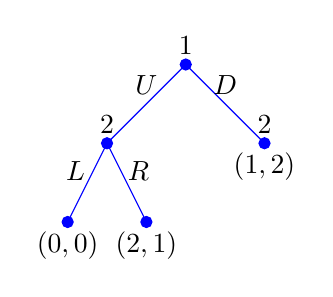
\begin{tikzpicture}
			\filldraw[blue] (0,0) circle(2pt);
			\filldraw[blue] (-1,-1) circle(2pt);
			\filldraw[blue] (1,-1) circle(2pt);
			\filldraw[blue] (-1.5,-2) circle(2pt);
			\filldraw[blue] (-.5,-2) circle(2pt);
			\draw[blue] (1,-1)--(0,0)--(-1,-1)--(-1.5,-2)--(-1,-1)--(-0.5,-2);
			\node[above] at (0,0) {$1$};
			\node[above] at (-1,-1) {$2$};
			\node[above] at (1,-1) {$2$};
			\node[above] at (-0.5,-0.5) {$U$};
			\node[above] at (0.5,-0.5) {$D$};
			\node[above] at (-0.6,-1.6) {$R$};
			\node[above] at (-1.4,-1.6) {$L$};
			\node[below] at (-1.5,-2) {$(0,0)$};
			\node[below] at (-0.5,-2) {$(2,1)$};
			\node[below] at (1,-1) {$(1,2)$};
		\end{tikzpicture}
		\caption{Simple Extensive Game}
		\label{fig:extensive_game_simple}
	\end{figure}
\end{example}


\begin{definition}
	A \blue{strategy} of a player $i$ in an extensive game with perfect information is a function $s_i(h) \to A(h)$ for any $h \in H \setminus Z$ such that $P(h) = i$. A strategy specifies an action for any node in which a player is asked to choose an action. A \blue{strategy profile} $s = (s_1,\dots,s_N)$. For each strategy profile, an \blue{outcome} $O(s)$ is the terminal node associated with the strategy profile. Note that we consider only pure strategies. If we consider mixes, then the outcome may be a distribution over terminal histories.
\end{definition}

\begin{definition}
	The \blue{strategic form} of an extensive game with perfect information $\langle N,\mathcal{H},P,\{u_i\}\rangle$ is the strategic game $\langle N,\{S_i\},\{\tilde{u}_i\}\rangle$ in which $S_i$ is the set of strategies in the extensive game, and $\tilde{u}_i(s) = u_i(O(s))$.
	
	A \blue{Nash equilibrium of an extensive game} is a Nash equilibrium of the associated strategic game.
\end{definition}


\begin{example}
	\red{Extensive Game with Strategic Form} Let's consider a modification to the previous example, in Figure~\ref{fig:modified_extensive_game_simple}.
	\begin{figure}[H]
		\centering
		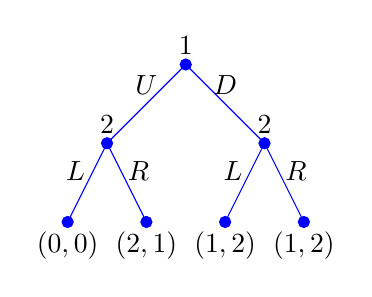
\begin{tikzpicture}
			\filldraw[blue] (0,0) circle(2pt);
			\filldraw[blue] (-1,-1) circle(2pt);
			\filldraw[blue] (1,-1) circle(2pt);
			\filldraw[blue] (-1.5,-2) circle(2pt);
			\filldraw[blue] (-.5,-2) circle(2pt);
			\filldraw[blue] (1.5,-2) circle(2pt);
			\filldraw[blue] (.5,-2) circle(2pt);
			\draw[blue] (1,-1)--(0,0)--(-1,-1)--(-1.5,-2)--(-1,-1)--(-0.5,-2);
			\draw[blue] (0.5,-2)--(1,-1)--(1.5,-2);
			\node[above] at (0,0) {$1$};
			\node[above] at (-1,-1) {$2$};
			\node[above] at (1,-1) {$2$};
			\node[above] at (-0.5,-0.5) {$U$};
			\node[above] at (0.5,-0.5) {$D$};
			\node[above] at (-0.6,-1.6) {$R$};
			\node[above] at (-1.4,-1.6) {$L$};
			\node[below] at (-1.5,-2) {$(0,0)$};
			\node[below] at (-0.5,-2) {$(2,1)$};
			\node[above] at (0.6,-1.6) {$L$};
			\node[above] at (1.4,-1.6) {$R$};
			\node[below] at (0.5,-2) {$(1,2)$};
			\node[below] at (1.5,-2) {$(1,2)$};
		\end{tikzpicture}
		\caption{Modified Simple Extensive Game}
		\label{fig:modified_extensive_game_simple}
	\end{figure}
	
	The strategic form game is
	\begin{center}
		\begin{tabular}{c|cccc}
			& $LL$ & $LR$ & $RL$ & $RR$ \\\hline
			$U$ & $(0,0)$ & $(0,0)$ & $(2,1)$ & $(2,1)$ \\
			$D$ & $(1,2)$ & $(1,2)$ & $(1,2)$ & $(1,2)$ 
		\end{tabular}
		
	\end{center}
	Here, $LL$ stands for $s_2(U) = L$, $s_2(D) = L$; $LR$ stands for $s_2(U) = L$, $s_2(D) = R$, and so on. Nash equilibria of the game are $(U,RL)$, $(U,RR)$, $(D,LL)$, and $(D,LR)$.
\end{example}

\begin{definition}
	Define two strategies $s_i$ and $s_i'$ as \blue{equivalent} if for each $s_{-i}$ we have $u_i(s_i,s_{-i}) = u_i(s_i',s_{-i})$.
\end{definition}
\begin{definition}
	The \blue{reduced form} of an extensive game is where we include only one member for each set of equivalent strategies. To wit:
	\begin{center}
		\begin{tabular}{c|cc}
			& $L$ & $R$ \\\hline
			$U$ & $(0,0)$ & $(2,1)$ \\
			$D$ & $(1,2)$ & $(1,2)$
		\end{tabular}
	\end{center}
\end{definition}

\begin{remark}
	There are some problems with the Nash solution here. If player 1 chooses $U$, it's natural to think that player 2 will choose $R$. However, the equilibria $(D,LL)$ and $(D,LR)$ exist based on the conjecture that if player 1 chose $U$, player 2 would select $L$. That's clearly not going to happen, by rationality.
\end{remark}

\begin{definition}
	The \blue{subgame} of an extensive game with perfect information $\Gamma$ that follows from history $h$ is the extensive form game $\Gamma(h) = \langle N,\mathcal{H}\mid_h, P\mid_h,\{u_i\}\mid_h\rangle$, where $\mathcal{H}\mid_h$ is the set of sequences $h'$ of actions for which $(h,h') \in \mathcal{H}$, $P\mid_h$ is such that $P\mid_h(h') = P(h,h')$ for $(h,h') \in \mathcal{H}$, and $u_i(h';h) \ge u_i(h'';h) \Longleftrightarrow u_i(h,h') \ge u_i(h,h'')$.
\end{definition}

\begin{definition}
	A \blue{subgame perfect equilibrium} is a strategy profile $s\opt$ in $\Gamma$ in which for any history $h$ the strategy profile $s\opt \mid_h$ is a Nash equilibrium of the subgame $\Gamma(h)$, where $s\opt \mid_h(h') = s\opt(h,h')$.
\end{definition}

\begin{example}
	\red{Stackelberg} Two firms 1 and 2 choose output levels $q_i \in [0,\infty)$. Firm 1 moves first, and the price is $p(q_1,q_2)$, so profit is $u_i(q_1,q_2) = q_i \cdot p(q_1,q_2) - c_i(q_i)$. To find a Nash equilibrium we find the reaction functions $r_2(q_1)$: \[p(q_1 + r_2(q_1)) + p'(q_1 + r_2(q_1)) - c_1'(r_2(q_1)) = 0\]and if we assume linear costs and demand we have that \[r_i(q_{-i}) = \frac{1 - q_{-i} - c}{2}\]Assume that 1 chooses first, and then 2. Now firm 1 optimizes knowing firm 2's reaction function, so they maximize \[q_1 \cdot \barl 1 - q_1 - \frac{1-q_1-c}{2}\barr - cq_1 = q_1 \barl \frac{1-q_1-c}{2}\barr - cq_1\]From the FOC, $(1 - 2q_1 + c) / 2 = c$, so $q	_1 = (1-c)/2$ and $q_2 = (1-c)/4$.
\end{example}

\begin{remark}
	To verify that a strategy $s\opt$ is a subgame perfect equilibrium, we need to check that for every $i \in N$ and every subgame $\Gamma(h)$, no strategy gives a strictly positive deviation. The following simplifies the calculation, by reducing the class of deviations we need to check.
\end{remark}

\begin{theorem}
	\red{One-Shot Deviation Principle} In a finite extensive game with observed actions, a strategy profile $s$ is a subgame perfect Nash equilibrium if and only if no player can strictly gain by deviating from $s$ in a single stage and conforming to $s$ thereafter.
\end{theorem}
\begin{proof}
	We want to show that $s$ is a subgame perfect equilibrium if and only if there is no $i$ and no $\hat{s}_i$ that agrees with $s_i$ except at a single $t$ and $h^t$ and such that $\hat{s}_i$ is a better response to $s_{-i}$ than $s_i$ conditionally on $h^t$. The forward direction is immediate. We will focus on the backwards direction.
	
	Proof by contrapositive: If $s$ is not a subgame perfect equilibrium, then $s$ violates the one-shot deviation principle. Suppose that $s$ is not a subgame perfect equilibrium, meaning that there is a $t$ and an $h^t$ such that some $i$ has a deviation $\hat{s}_i$ in the subgame $\Gamma(h^t)$. Let $\hat{t}$ be the largest $t$ such that $\hat{s}_i(h^t) \ne s_i(h^t)$ (which exists because the game is finite). Consider an alternative strategy $\tilde{s}_i$ that agrees with $\hat{s}_i$ for all $t < \hat{t}$ and agrees with $s_i\mid_{h^t}$ from $\hat{t}$ on. 
	
	Since from any $h^{\hat{t}}$ it agrees with $s_i \mid_{h^{\hat{t}}}$ except for the first move, by the one-shot deviation principle this change can only increase the utility of $i$ at any $h^{\hat{t}}$. Of course if the principle fails we are done, so assume that it does not. This means that $\tilde{s}_i$ is as good as $\hat{s}_t$ at $h^{t}$. If $\hat{t} = t+1$, then $\tilde{s}_i = s_i$ and we have a contradiction. If $\hat{t} > t+1$, then iterate the procedure until we have a contradiction. 
\end{proof}

\begin{remark}
	With no additional assumptions, this theorem fails in the infinite horizon case. Consider the following example, illustrated in Figure~\ref{fig:one_shot_example}, where the payoff of playing infinite $a$ is 1.
	\begin{figure}[H]
		\centering
		\begin{tikzpicture}[scale=0.5]
			\draw[blue,thick] (0,0)--(0,5)--(20,5);
			\draw[blue,thick,dashed] (20,5)--(22.5,5);
			\draw[blue,thick] (5,5)--(5,0);
			\draw[blue,thick] (10,5)--(10,0);
			\draw[blue,thick] (15,5)--(15,0);
			\filldraw[blue] (0,0) circle(4pt);
			\filldraw[blue] (0,5) circle(4pt);
			\filldraw[blue] (5,0) circle(4pt);
			\filldraw[blue] (10,0) circle(4pt);
			\filldraw[blue] (15,0) circle(4pt);
			\filldraw[blue] (5,5) circle(4pt);
			\filldraw[blue] (10,5) circle(4pt);
			\filldraw[blue] (15,5) circle(4pt);
			\filldraw[blue] (20,5) circle(4pt);
			\node[left] at (0,2.5) {$d$};
			\node[left] at (5,2.5) {$d$};
			\node[left] at (10,2.5) {$d$};
			\node[left] at (15,2.5) {$d$};
			\node[above] at (2.5,5) {$a$};
			\node[above] at (7.5,5) {$a$};
			\node[above] at (12.5,5) {$a$};
			\node[above] at (17.5,5) {$a$};
			\node[below] at (0,-0.2) {$0$};
			\node[below] at (5,-0.2) {$0$};
			\node[below] at (10,-0.2) {$0$};
			\node[below] at (15,-0.2) {$0$};
			\node[right] at (22.5,5) {$1$};
		\end{tikzpicture}
		\caption{Infinite Game with no One-Shot Deviations}
		\label{fig:one_shot_example}
	\end{figure}
	The strategy $d$ after every history satisfies the one-shot deviation principle, but is clearly not a subgame perfect Nash equilibrium. To ensure that the one-shot deviation principle applies to infinite games, we need the following definition:
\end{remark}

\begin{definition}
	A game is \blue{continuous at infinity} if for each player $i$ the utility function $u_i(h)$ satisfies \[\sup_{h,\hat{h} \st h^t = \hat{h}^t} \Big| u_i(h) - u_i(\hat{h}) \Big| \to 0 \text{ as } t \to \infty \]where $h,\hat{h}$ are infinite histories and $u_i(h),u_i(\hat{h})$ their respective utilities. Note that this condition is satisfied if the utilities are equal to a discounted sum of per-period payoffs $U_i^t(a^t)$ that are uniformly bounded.
\end{definition}

\begin{theorem}
	\red{One-Shot Deviation Principle for Infinite Games} In an infinite horizon extensive game with observed actions that is continuous at infinity, a strategy profile $s$ is a subgame perfect Nash equilibrium if and only if no player can strictly gain by deviating from $s$ in a single stage and conforming to $s$ thereafter.
\end{theorem}


\begin{theorem}
	\red{Kuhn's Theorem} Every finite extensive game with perfect information has a subgame perfect equilibrium.
\end{theorem}
\begin{proof}
	(Constructive) We have a finite extensive game $\Gamma$ with subgames $\{\Gamma(h)\}$, which are finite. Define $\ell(\Gamma(h))$ the length of the maximal history of $\Gamma(h)$. We now define $R(h)$ as a function which associates a terminal history $h'$ to every history $h$ such that $h' \succeq h$. 
	
	When $\ell(\Gamma(h)) = 0$, then we are in a terminal history and $R(h) = h$. Now assume we have defined $R(h)$ for all $h$ with $\ell(\Gamma(h)) \le k$. Consider an $h'$ such that $\ell(\Gamma(h')) = k+1$. We have that $\ell(\Gamma(h',a)) \le k$ for all $a \in A(h')$. Let $s_i(h')$ be such that $u_i(R(h',s_i(h'))) \ge u_i(R(h',a))$ for all $a \in A(h')$. Define $R(h) = R(h',s_i(h'))$. We have defined by induction $R(h)$ and a strategy $s$ that is a subgame perfect equilibrium by the one-shot deviation principle.
\end{proof}

\begin{remark}
	This method is called \blue{backwards induction}. The intuition here is to solve the game from the end, from the most simple subgame.
\end{remark}

\begin{remark}
	We might also want to describe situations with some randomness -- where nature also moves. This is easily incorporated.
\end{remark}

\begin{definition}
	An \blue{extensive game with perfect information and chance moves} is a tuple $\langle N,\mathcal{H},P,f_c,\{\succeq_i\}\rangle$, where now (i) $P$ is a function from $\mathcal{H}$ to $N \cup \{c\}$ where $c$ is for chance, (ii) for each $h$ such that $P(h) = c$, $f_c(\cdot; h)$ is a probability distribution over $A(h)$, (iii) $\{\succeq_i\}$ are preferences over lotteries over terminal nodes. 
\end{definition}

\begin{remark}
	We can also introduce a similar concept which introduces some uncertainty even in a game with perfect information and no chance.
\end{remark}

\begin{definition}
	An \blue{extensive game with perfect information and simultaneous moves} is a tuple $\langle N, \mathcal{H}, P, \{u_i\}\rangle$ such that (i) $N$ is the set of players, (ii) $\mathcal{H}$ is a sequence of $|P(h)|$ dimensional vectors of actions, (iii) $P$ identifies the set of players who chose after history $h$, and (iv) $u_i$ is the same as before.
	
	A strategy is a function $s_i(h) \to A_i(h)$ for all $i \in P(h)$, and the definitions of subgames and subgame perfect equilibria apply here.
\end{definition}

\begin{remark}
	When we represent a game with simultaneous moves, we don't have perfect information. If we want to use a game tree representation, we need to describe this information. To this goal, we introduce:
\end{remark}

\begin{definition}
	\blue{Information sets} are partitions of the histories with the interpretation that a player at a node $x$ is unsure whether they are at $x$ or any other $x' \in z(x)$. The same player must move at $x$ and $x'$, and we must have that $A(x) = A(x')$ for it to be true that $x,x'\in z(x)$. 
\end{definition}

\begin{remark}
	Information sets can be used to describe information in a game tree. They could also describe situations in which information is degraded, meaning when a player might forget what they once knew. Games with perfect recall are games in which nobody forgets.
\end{remark}

\begin{remark}
	In a game with perfect information and simultaneous moves, we can generalize the one-shot deviation principle. However, we cannot guarantee the existence of a subgame perfect equilibrium in pure strategies. See: matching pennies.
\end{remark}

\begin{remark}
	A strategy specifies actions after nodes. Some histories can have zero probability given a player's strategy. We are requiring players to make choices even in situations that will never happen! We do this because it forms a basis for the beliefs of other players. The key assumption here is that rationality is still our guiding principle no matter what is observed.
\end{remark}

\begin{question}
	What happens when we end up in a history that has probability zero? What does that mean for the rationality of other players?
	
	And then: What does this imply for how the other players \emph{will} play? Perhaps they are irrational! That has implications for future play.
\end{question}

More generally: Past actions may be informative about how the opponents will play if there is some `ambiguity' in the continuation subgame. Iterated deletion of weakly dominated strategies may capture this type of reasoning.

\begin{example}
	\red{Battle of the Sexes (pt. 2)} Consider the following game, in extensive and normal form:
	\begin{figure}[H]
		\centering
		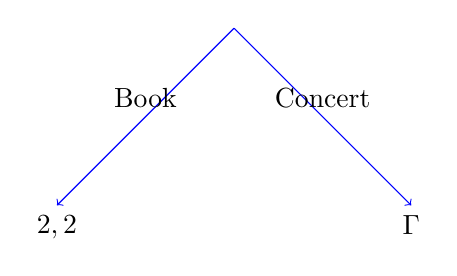
\begin{tikzpicture}[scale=0.75]
			\draw[blue,->](0,0)--(-3,-3);
			\draw[blue,->](0,0)--(3,-3);
			\node[below] at (-3,-3) {$2,2$};
			\node[below] at (3,-3) {$\Gamma$};
			\node[above] at (1.5,-1.5) {Concert};
			\node[above] at (-1.5,-1.5) {Book};
		\end{tikzpicture}
	\end{figure}
	where:
	\[\Gamma \equiv \qquad \begin{array}{c|cc} & \text{Bach} & \text{Stravinski} \\\hline \text{Bach} & $3,1$ & $0,0$ \\ \text{Stravinski} & $0,0$ & $1,3$ \\\end{array}\]
	The subgames are (Book,$S$),$S$ and (Concert,$B$),$B$. However, one is clearly more plausible than the other. We can see this in the strategic form of the full game:
	\begin{center}
	\begin{tabular}{c|cc}
	& $B$ & $S$ \\\hline 
	Book & $2,2$ & $2,2$ \\ $B$ & $3,1$ & $0,0$ \\ $S$ & $0,0$ & $3,1$  
	\end{tabular}	
	\end{center}
	Note that Book strictly dominates $S$ for 1, and after that $B$ weakly dominates $S$ for 2. This implies (heuristically) that Bach is much more likely than Book.
\end{example}


\begin{example}
	\red{BotS (Burning Money)} Consider the following game:
	\begin{figure}[H]
		\centering
		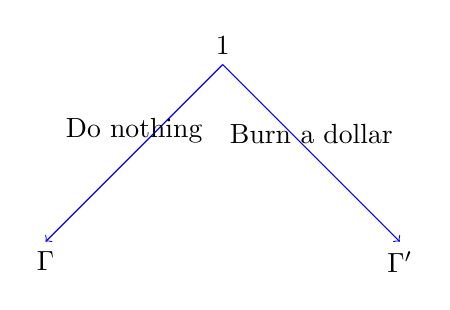
\begin{tikzpicture}[scale=0.75]
			\draw[blue,->](0,0)--(-3,-3);
			\draw[blue,->](0,0)--(3,-3);
			\node[below] at (-3,-3) {$\Gamma$};
			\node[below] at (3,-3) {$\Gamma'$};
			\node[above] at (1.5,-1.5) {Burn a dollar};
			\node[above] at (-1.5,-1.5) {Do nothing};
			\node[above] at (0,0) {$1$};
		\end{tikzpicture}
	\end{figure}
	where 
	\[\Gamma \equiv \qquad \begin{array}{c|cc} & \text{Bach} & \text{Stravinski} \\\hline \text{Bach} & $3,1$ & $0,0$ \\ \text{Stravinski} & $0,0$ & $1,3$ \\\end{array}\]
	and
	\[\Gamma' \equiv \qquad \begin{array}{c|cc} & \text{Bach} & \text{Stravinski} \\\hline \text{Bach} & $2,1$ & $-1,0$ \\ \text{Stravinski} & $-1,0$ & $0,3$ \\\end{array}\]
	where player 2 observes the choice to either do nothing or burn the dollar. We can solve this game with iterated deletion of strictly dominated strategies in the strategic form game:
	\begin{center}
		\begin{tabular}{c|cccc}
		&$BB$ &$BS$ & $SB$ & $SS$ \\\hline
		$DnB$ & $3,1$ & $3,1$ & $0,0$ & $0,0$ \\
		$DnS$ & $0,0$ & $0,0$ & $1,3$ & $1,3$ \\
		$BdB$ & $2,1$ & $-1,0$ & $2,1$ & $-1,0$\\
		$BdS$ & $-1,0$ & $0,3$ & $-1,0$ & $0,3$ 
		\end{tabular}
	\end{center}
	where $DnB$ weakly dominates $BdS$, and after that is eliminated $SB$ weakly dominates $SS$, so we end up with the unique pure-strategy Nash equilibrium in the game 
	\begin{center}
		\begin{tabular}{c|ccc}
		&$BB$ &$BS$ & $SB$  \\\hline
		$DnB$ & \boxed{$3,1$} & $3,1$ & $0,0$ \\
		$DnS$ & $0,0$ & $0,0$ & $1,3$ \\
		$BdB$ & $2,1$ & $-1,0$ & $2,1$
		\end{tabular}
	\end{center}
	What is the logic here? In the original battle of the sexes, a player can guarantee a payoff of \[\pi=\min_{\alpha\in[0,1]} \max \{3\alpha,1-\alpha\} = \frac{3}{4}\]In the original game, this is irrelevant. However, once the dollar has been burned, the only way for player 2 to guarantee this is by playing $B$. So if 1 burns the dollar they will play $B$, and if 1 does not burn the dollar 2 knows that they will play $B$, because otherwise they could do better by choosing to burn the dollar and guaranteeing 2.
\end{example}


\begin{example}
	\red{The Centipede Game} Two players are in a process that they can alternatively stop or continue. At each time $t$, each player prefers stopping now to letting the opponent stop at $t+1$. In the last period $t = T-1$, the player prefers stop to continue. However, the terminal history $T$ (attained by continuing at $T-1$) is better for both players than stopping at any $t < T-1$. One classical formulation is:
	\begin{figure}[H]
	\centering
		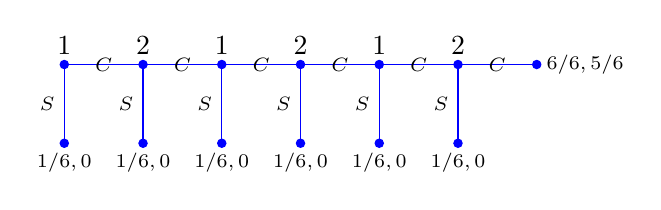
\begin{tikzpicture}
			\draw[blue] (0,0)--(6,0);
			\draw[blue] (0,0)--(0,-1);
			\draw[blue] (1,0)--(1,-1);
			\draw[blue] (2,0)--(2,-1);
			\draw[blue] (3,0)--(3,-1);
			\draw[blue] (4,0)--(4,-1);
			\draw[blue] (5,0)--(5,-1);
			\node[below] at (0,-1) {\scriptsize $1/6,0$};
			\node[below] at (1,-1) {\scriptsize $1/6,0$};
			\node[below] at (2,-1) {\scriptsize $1/6,0$};
			\node[below] at (3,-1) {\scriptsize $1/6,0$};
			\node[below] at (4,-1) {\scriptsize $1/6,0$};
			\node[below] at (5,-1) {\scriptsize $1/6,0$};
			\node[right] at (6,0) {\scriptsize $6/6,5/6$};
			\node[above] at (0,0) {$1$};
			\node[above] at (1,0) {$2$};
			\node[above] at (2,0) {$1$};
			\node[above] at (3,0) {$2$};
			\node[above] at (4,0) {$1$};
			\node[above] at (5,0) {$2$};
			\node at (0.5,0) {\scriptsize $C$};
			\node at (1.5,0) {\scriptsize $C$};
			\node at (2.5,0) {\scriptsize $C$};
			\node at (3.5,0) {\scriptsize $C$};
			\node at (4.5,0) {\scriptsize $C$};
			\node at (5.5,0) {\scriptsize $C$};
			\node[left] at (0,-0.5) {\scriptsize $S$};
			\node[left] at (1,-0.5) {\scriptsize $S$};
			\node[left] at (2,-0.5) {\scriptsize $S$};
			\node[left] at (3,-0.5) {\scriptsize $S$};
			\node[left] at (4,-0.5) {\scriptsize $S$};
			\node[left] at (5,-0.5) {\scriptsize $S$};
			\filldraw[blue] (0,0) circle(1.5pt);
			\filldraw[blue] (1,0) circle(1.5pt);
			\filldraw[blue] (2,0) circle(1.5pt);
			\filldraw[blue] (3,0) circle(1.5pt);
			\filldraw[blue] (4,0) circle(1.5pt);
			\filldraw[blue] (5,0) circle(1.5pt);
			\filldraw[blue] (6,0) circle(1.5pt);
			\filldraw[blue] (0,-1) circle(1.5pt);
			\filldraw[blue] (1,-1) circle(1.5pt);
			\filldraw[blue] (2,-1) circle(1.5pt);
			\filldraw[blue] (3,-1) circle(1.5pt);
			\filldraw[blue] (4,-1) circle(1.5pt);
			\filldraw[blue] (5,-1) circle(1.5pt);
		\end{tikzpicture}
	\end{figure} 
	There is a unique subgame-perfect equilibrium: $s_i(h^t) = S$ for all $i,t$. Any pair of strategies in which player 1 chooses $S$ in the first period and player 2 chooses $S$ in the second is a Nash equilibrium. Is this realistic? 
\end{example}
\begin{remark}
	One way to reconcile the experimental observations is to note that cooperation is close to an equilibrium as long as the game is sufficiently long.
\end{remark}
\begin{definition}
	A profile $s\opt$ is an \blue{$\varepsilon$-Nash equilibrium} if, for all players $i$ and strategies $s_i$, we have \[u_i(s\opt) \ge u_i(s_i,s_{-i}\opt) - \varepsilon\]for some $\varepsilon > 0$. 
\end{definition}

\begin{example}
	Consider the centipede game with $T$ stages, so payoffs go to $T, T-1$, and normalize by dividing by $T$. Is cooperation up to $k$ (for some $k$) optimal if $T$ is sufficiently large? No deviation is optimal for $T \ge k$, since the strategy recommends to stop, and no deviation is optimal for $T \le k-2$, since it is optimal to continue if the other player will continue. Finally, at $\tau = k-1$, the net benefit of a deviation is $1/T$, and for $T$ sufficiently large $1/T < \varepsilon$. So this is an $\varepsilon$-Nash equilibrium. 
\end{example}

\subsection{Notable Dynamic Models}

\begin{model}
	\red{Rubinstein Bargaining} (from \href{https://arielrubinstein.tau.ac.il/papers/11.pdf}{Rubinstein (1982)}) Two players must split a pie of size 1. They alternate making offers: in even periods $t = 0,2,4,\dots$, Player 1 proposes $(x,1-x)$ where $x$ is the share allocated to Player 1. If Player 2 accepts, the payoffs are $(x,1-x)$; and in odd periods $t = 1,3,5,\dots$, Player 2 proposes $(1-x,x)$, and Player 1 can accept or reject, and so on. We denote by $x_j^i$ the amount allocated by player $i$ to player $j$ -- so in Period 1, $x^1_1 = x$, and $x^1_2 = 1-x$. In each period, payoffs are discounted by $(\delta_1,\delta_2)$ respectively, so payoffs for an allocation $(x,y)$ in period $t$ will be $(\delta_1^t x, \delta_2^t y)$.
	
	\begin{remark}
		There are many Nash equilibria in this game (in fact, every $x\in [0,1]$ admits a Nash equilibrium $(x,1-x)$), but only one subgame perfect equilibrium. This restriction is what makes non-cooperative bargaining games tractable.
	\end{remark}
	
	Consider the set of strategies: 1 always demands 1 and refuses anything less; 2 demands 0 and accepts anything. This is a Nash equilibrium (weakly, for 2, but still Nash), but is clearly not subgame perfect. In fact, any $x$ proposed by 1 would be a Nash equilibrium with these same strategies. To show that it is not subgame perfect, observe: if 2 rejects the offer, they can offer $x \in (\delta,1)$, where it is rational for 1 to accept since $u_1(x) = x > \delta = \delta u_1(1)$. 
	
	Here is a subgame perfect equilibrium (we will show that this is a subgame perfect equilibrium, and then that this is the unique subgame perfect equilibrium): Player $i$ always demands a share \[x_i^i = \frac{1-\delta_j}{1-\delta_i\delta_j}\]when she makes an offer. Player $i$ always demands \[x_i^j = \frac{\delta_i(1-\delta_j)}{1-\delta_i\delta_j}\]when she does not make an offer. First, we want to prove that this is a Nash equilibrium in any possible subgame. Usefully, there are only two subgames that are relevant -- when $i$ is the proposer and when $i$ is the receiver. We will apply the one-stage deviation principle. All the other subgames are symmetric. Let's check the proposer deviations. Any proposal must satisfy\[1-\tilde{x}^i_i \ge x^i_j = \frac{\delta_j(1-\delta_i)}{1-\delta_j\delta_i} = 1 - \frac{1-\delta_j}{1-\delta_i\delta_j} = 1-x_i^i \Longleftrightarrow \tilde{x}^i_i \le x_i^i\]Since $i$ knows that $x^i_i$ is accepted, it must be the case that $\tilde{x}^i_i \ge x^i_i$. Thus, this is either not profitable or not a deviation. Similarly, Player 2 refuses if \[\tilde{x}^i_j < \delta_j x^j_j = \frac{\delta_j(1-\delta_i)}{1-\delta_i\delta_j} = x_j^i\]and is willing to accept otherwise. 
	
	Rubinstein's key result is that this is the unique SPE. To see this, let $\bar{v}_i$ and $\underline{v}_i$ to be player $i$'s supremum and infimum payoffs in the set of possible payoffs in a SPE. We must have that $\underline{v}_1 \ge 1 - \delta_2 \bar{v}_2$, since 2 would always accept anything larger than $\delta_2\bar{v}_2$. Similarly, we must have that $\underline{v}_2 \ge 1-\delta_1\bar{v}_1$. Moreover, we must have that \[\bar{v}_1 \le \max\{1-\delta_2\underline{v}_2, \delta_1^2 \bar{v}_1\}\]The first inequality $\bar{v}_1 \le 1-\delta_2 \underline{v}_2$ means that 2 rejects anything that gives her less than $\delta_2 \underline{v}_2$, implying that $1-x^1_1 \ge \delta_2 \underline{v}_2$. The second follows from the fact that 1 can go for a rejected offer and wait one turn. So this implies that \[\bar{v}_i \le 1-\delta_j \underline{v}_j\]Combining the inequalities, we have that\[\underline{v}_i \ge 1-\delta_j \bar{v}_j \le 1-\delta_j(1-\delta_i)\underline{v}_i \Longrightarrow \underline{v}_i \le \frac{1-\delta_j}{1-\delta_i\delta_j}\]\[\bar{v}_i \le 1-\delta_j \underline{v}_j \ge 1-\delta_j(1-\delta_i)\bar{v}_i \Longrightarrow \bar{v}_i \le \frac{1-\delta_j}{1-\delta_i\delta_j}\]So thus, we have that \[\bar{v}_i = \underline{v}_i = \frac{1-\delta_j}{1-\delta_i\delta_j}\]
	
	\begin{remark}
		There are no mixed equilibria -- even though the receiver is indifferent between accepting and rejecting, as soon as they decide to mix the best strategy for the sender will be to propose $\min\{(\delta_j v_j,1]\}$, which is empty.
	\end{remark}
	
	\begin{remark}
		The unique payoff is determined by the discount factors and the order of play -- the more patient player will attain higher payoff, and the first proposer will attain higher payoff in equilibrium. Note that the first mover advantage attenuates as $\delta \to 1$. 
	\end{remark}
	\end{model}


\begin{definition}
	Often a game is played repeatedly over time. In this case, the game that is played repeatedly is called the \blue{stage game} and the overall game is called the \blue{repeated game}.
\end{definition}

\begin{remark}
	Even when this is done in finite horizons or the game has a unique equilibrium, this may lead to a larger set of equilibria. Repetitions allow the players to condition their actions on the actions taken by players in previous periods. In fact, even if the past actions are payoff irrelevant (meaning they do not affect the payoffs), conditioning on past actions makes the strategies \blue{interactive} and thus more powerful. Equilibria may be associated to payoffs that are higher or lower for all players than the payoff in the unique equilibrium of the stage game.
\end{remark}


\begin{example}
	\red{Repeated Prisoner's Dilemma}. Recall:
	\begin{center}
		\begin{tabular}{c|cc}
		& $C$ & $D$ \\\hline 
		$C$ & $(1,1)	$ & $(-1,2)$ \\
		$D$ & $(2,-1)$ & $(0,0)$
		\end{tabular}
	\end{center}
	Defect is the unique equilibrium in the stage game. Note that past actions are payoff irrelevant -- the way you played in the past does not affect the payoffs in the future. Consider the repeated version of the game, where strategies are functions of past actions $a^t$: $\sigma_i(a^t)$. If the game is repeated for $T$ periods, we can write the payoff as \[U_i = \frac{1-\delta}{1-\delta^{T+1}} \sum_{t=0}^T \delta^t u_i(\sigma(a^t))\]where the first term allows us to express the payoffs as \blue{average discounted payoffs}. As $T \to \infty$, we have that \[U_i = (1-\delta) \sum_{t=0}^\infty \delta^t u_i(\sigma(a^t))\]We claim that, as $T \to \infty$ when $\delta \ge 0.5$ there exists a subgame perfect equilibrium in which both players choose cooperate in equilibrium. An obvious SPE is playing defect forever. Consider the following \blue{grim trigger} strategies. Player $i$ plays $C$ forever, but if player $j$ plays $D$ in some period $t$, Player $i$ plays $D$ for period $t+1$ and thenceforth forever.
	
	To see that this is a subgame perfect equilibrium, consider deviations. If we are in the first state, playing $C$ forever, then the payoffs for $i$ are\[u_i(C) = (1-\delta) \sum_{t=0}^\infty \delta^t = 1 \ge (1-\delta) [2 + 0 + \cdots] = 2(1-\delta)\]so as long as $\delta \ge 0.5$, $C$ is weakly preferred. If we are in the second state, the strategy prescribes playing $D$ forever, which is the stage game dominant strategy, so of course is an equilibrium. Note that we can obtain a strictly higher payoff in equilibrium than the stage game Nash strategies get.
	
	\begin{remark}
		The (possible) average payoffs of the two players can be represented in two dimensions:
		\begin{figure}[H]
			\centering
			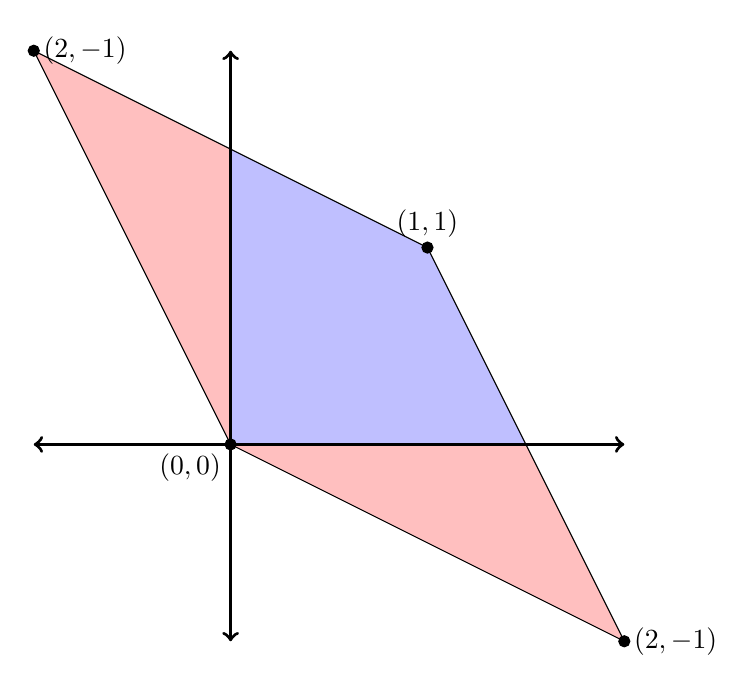
\begin{tikzpicture}[scale=0.5]
				\fill[blue, nearly transparent] (5,5)--(0,7.5)--(0,0)--(7.5,0)--(5,5);
				\fill[red, nearly transparent] (0,7.5)--(-5,10)--(0,0)--(0,7.5);
				\fill[red, nearly transparent] (7.5,0)--(10,-5)--(0,0)--(7.5,0);
				\draw[very thick, <->] (10,0)--(-5,0);
				\draw[very thick, <->] (0,10)--(0,-5);
				\draw[black] (5,5)--(-5,10)--(0,0)--(10,-5)--(5,5);
				\filldraw[black] (5,5) circle(4pt);
				\filldraw[black] (-5,10) circle(4pt);
				\filldraw[black] (10,-5) circle(4pt);
				\filldraw[black] (0,0) circle(4pt);
				\node[above] at (5,5) {$(1,1)$};
				\node[right] at (10,-5) {$(2,-1)$};
				\node[right] at (-5,10) {$(2,-1)$};
				\node[below left] at (0,0) {$(0,0)$};
				
			\end{tikzpicture}
		\end{figure}
		where the shaded areas show the convex hull of the stage payoffs, the blue shows the average payoffs attainable by a rationalizable strategy (the \blue{Folk Theorem}).
	\end{remark}
\end{example}



\begin{example}
	\red{Carrot and Stick} Consider the following game:
	\begin{center}
		\begin{tabular}{c|ccc}
			& A & B & C \\\hline 
			A & 2,2 & 2,1 & 0,0 \\
			B & 1,2 & 1,1& -1, 0 \\
			C & 0,0 & 0,-1 & -1,-1
		\end{tabular}
	\end{center}
	This game has the unique equilibrium $(A,A)$, getting payoffs $(2,2)$. However, consider the following SPE: In State I, Play $B$ unless the other does something different. If they deviate, go to State II, where you play $C$. If all others play $C$, return to State I. If not, stay in State II. Suppose we are in State I. Then payoffs for $B$ are $(1-\delta) \sum_{t=0}^\infty \delta^t = 1$, while the best deviation yields $2 - \delta + \delta^2 + \delta^3 + \cdots = 1 + (1-\delta)(1-2\delta)$ so $B$ is preferred as long as  $\delta \ge 1/2$. In State II, the payoffs are:
	\begin{align*}
		u(C) &= (1-\delta) [-1 + \delta + \delta^2 + \cdots] = 1 - 2(1-\delta) \\u(B) < u(A) &= (1-\delta) [0 - \delta + \delta^2 + \cdots] = 1 + (1-\delta)(1-2\delta)
	\end{align*}
	So $C$ is optimal again as long as $\delta \ge 1/2$. 
\end{example}

\begin{example}
	\red{Multiple Equilibria in a Finite Game} Consider: 
	\begin{center}
		\begin{tabular}{c|ccc}
			& A & B & C \\\hline
			A & 0,0 & 3,4 & 6,0 \\
			B & 4,3 & 0,0 & 0,0 \\
			C & 0,6 & 0,0 & 5,5
		\end{tabular}
	\end{center}
	This game has two pure equilibria: $(B,A)$ and $(A,B)$, and a mixed equilibrium $(3/7 A + 4/7 B, 4/7 A + 3/7 B)$. Note that all payoffs fall short of the maximal, $(5,5)$. In the twice-repeated game, we have a SPE that leads to the maximal payoff $(5,5)$: The strategies are to play $C$ at $t=1$, and if $(C,C)$ is attained play $(B,A)$ at $t=2$. Otherwise, play the mixed equilibrium strategy. In equilibrium, payoffs are $(5,5) + \delta(4,3)$, and the gain from a deviation is (at most) $1$ at $t=1$, with a loss of at minimum $\delta(3 - 12/7)$. The strategies are a SPE if $\delta(3-12/7) > 1 \Longleftrightarrow \delta \ge 7/9$.
\end{example}

\begin{example}
	\red{War of Attrition} Two animals are fighting for a prize with value $v$. The fighting cost is 1 per period. If an animal stops fighting at $t$, the opponent wins $v$, there is no fighting, and the game stops. There is a per-period discount factor $\delta$. The payoff of quitting at time $\hat{t}$ is\[L(\hat{t}) = - (1 + \delta + \delta^2 + \cdots + \delta^{\hat{t}-1})\]the payoff of the winner is \[W(\hat{t}) = - (1 + \delta + \delta^2 + \cdots + \delta^{\hat{t}-1}) + \delta^{\hat{t}}v = L(\hat{t}) + \delta^{\hat{t}}v\]If both animals quit together, we assume the payoff is $L(\hat{t})$ for both. 
	
	As in the bargaining game, here we have several Nash equilibria. For example: $i$ always fights, $j$ always stops. This is a Nash equilibrium and is subgame perfect. Is the game indeterminate? If we look for a symmetric equilibrium, there is one unique one, in the form of stopping with probability $p$ in each period where the game is continuing. It is easy to see that $p \in (0,1)$. In equilibrium, we must have that\[L(t) = pW(t) + (1-p)L(t+1) \Longleftrightarrow L(t) - L(t+1) = p[W(t) - L(t+1)]\]where the left hand side is the payoff of stopping and the right is the payoff of continuing. Simplifying, we have that this becomes \[\delta^t = p(\delta^t + \delta^tv) \Longleftrightarrow p\opt = \frac{1}{1+v}\]
\end{example}
\begin{remark}
	Note that both the symmetric and asymmetric equilibria we have seen so far are stationary. A stationary Nash equilibrium is always a Nash equilibrium, since subgames are all strategically equivalent.
\end{remark}



\section{Repeated Games}

\subsection{Folk Theorems}

Let $G$ be a normal form game with action spaces $A_1,\dots,A_I$, payoff functions $g_i: A \to \reals$, where $A = \bigtimes_i A_i$. Let $G^\infty(\delta)$ be the infinitely repeated version of $G$ played at $t= 0,1,2,\dots$ where players discount at $\delta$ and observe all previous actions. A history is $\mathcal{H}^t = \{a^0,a^1,\dots,a^{t-1}\}$, and a pure strategy is $s_{i,t} : \mathcal{H}^t \to A_i$. The average discounted payoff is \[u_i(a_i,s_{-i}) = (1-\delta) \sum_{t=0}^\infty \delta^t g_i(s_i(h^t),s_{-i}(h^t))\]Our goal is to study the set of average payoffs that are associated to SPE of the repeated game as a function of $\delta$. A few constraints immediately bound this set:

\begin{definition}
	The \blue{set of feasible payoffs} is the set of vectors $C \subseteq \reals^I$ \[(v_1,\dots,v_I) \in \text{Co}\{ (v_1,\dots,v_I) : \exists (a_1,\dots,a_I) \st g_i(a) = v_i \forall i\}\]where Co$\{\cdot\}$ denotes the convex hull of $\{\cdot\}$. Naturally, the set of equilibria must be included in this set.
\end{definition}

Another constraint is individual rationality:

\begin{definition}
	A player's \blue{min-max} payoff is \[\underline{v}_i = \min_{s_{-i}}\max_{s_i} g_i(s_i,s_{-i})\]where here $s_i$ is a mixed strategy.
\end{definition}

\begin{definition}
	A payoff vector is \blue{individually rational} if $v_i \ge \underline{v}_i \forall i$.
\end{definition}

\begin{lemma}
	Any Nash equilibrium must be individually rational.
\end{lemma}
\begin{proof}
	Suppose that $s\opt$ is a Nash equilibrium, where for some $i$ $v_i < \underline{v}_i$. Then we have that there exists some other $s_i'$ that attains a strictly higher payoff for any $s_{-i}$, including $s_{-i}\opt$. Thus, $s_i\opt$ would not be a best response, and $i$ would deviate for $s_i'$.
\end{proof}

We will start with the classic framework, which will highlight some of the key ideas. However, it's not nearly as nice as the SPE Folk result we will see later.

\begin{theorem}
	\red{Folk Theorem in Nash Equilibria} If $ v=(v_1,\dots,v_I)$ is feasible and strictly individually rational, then there exists $\delta\opt < 1$ such that for all $\delta > \delta\opt$, there is a Nash equilibrium of $G^\infty (\delta)$ with average payoffs $(v_1,\dots,v_I)$. 
\end{theorem}
\begin{proof}
	Assume that there exists a profile $a$ such that $g_i(a) = v_i$ for all $i$. This is for simplicity and not without loss,\footnote{It does hold if we have either a continuum of actions or a randomization device.} we will return to this later. Let $m_{-j}^j$ be the strategy profile of players other than $j$ that holds $j$ to at most $\underline{v}_j$, and write $m_j^j$ for $j$'s best response to $m_{-j}^j$. Let $m^j = (m^j_j,m^j_{-j})$. Now consider the following strategies: \begin{itemize} \item State I: Play $a$ if there was no deviation or if there was more than one deviation \item  State II: if $j$ deviates, play $m^j$ forever \end{itemize}We can verify this is a Nash equilibrium using one-stage deviation. If $a$ is played, then $j$ receives \[(1-\delta) \parl v_j + \frac{\delta}{1-\delta} v_j\parr = v_j\]If there is a deviation, then $j$ receives \[(1-\delta) \parl \bar{v}_j + \frac{\delta}{1-\delta} \underline{v}_j\parr\]so deviation is not profitable if and only if \[(1-\delta)(\bar{v}_j - v_j) \le \delta (v_j - \underline{v}_j)\]As $\delta \to 1$, the left hand side goes to zero, so this condition holds for sufficiently large $\delta$. Note that we are using the fact that $v$ is \emph{strictly} individually rational here.
\end{proof}

\begin{remark}
	The issue here is that we are asking players to minimax after a deviation -- but that might not be a Nash equilibrium of the subgame in question, so would not be a credible threat. See the example:
	\begin{center}
		\begin{tabular}{c|cc}
			& A & B \\\hline A & 8,8 & 0,-50 \\ B & 10,1 & 0,-50
		\end{tabular}
	\end{center}
	Note here that $\underline{v}_1 = 0$ and $\underline{v}_2 = 1$. So despite the fact that $(8,8)$ is feasible and individually rational, the Nash Folk Theorem says we can achieve it as a Nash equilibrium, but the minimax threat is not credible (as 2 would get $-50$ forever!).
\end{remark}

\begin{theorem}
	\red{SPE Folk Theorem} \emph{(from \href{https://scholar.harvard.edu/files/maskin/files/folk_theorem_in_repeated_games_with_discounting_or_incomplete_information.pdf}{Fudenberg and Maskin (1986)})} Let $V\opt$ be the set of feasible and strictly individually rational payoffs. Assume that $\dim V\opt = I$. Then for any $(v_1,\dots,v_I) \in V\opt$, there exists $\delta\opt < 1$ such that for any $\delta > \delta\opt$, there is a subgame perfect equilibrium of $G^\infty(\delta)$ with average payoffs $(v_1,\dots,v_I)$.
\end{theorem}
\begin{proof}
	Fixing a payoff vector $v \in V\opt$, we construct a SPE that achieves it. For convenience (and again with only a small loss), assume that there is a strategy profile $a$ such that $g_i(a) = v_i$ for all $i$. Choose $v' \in \interior(V\opt)$ such that $\underline{v}_i < v_i' < v_i$ for all $i$. We choose $N$ such that \[\max_a g_i(a) + N\underline{v}_i < \min_a g_i(a) + Nv'_i\]We choose $\varepsilon > 0$ such that for each $i$,\[v'(i) = (v'_1 + \varepsilon,\dots,v'_{i-1} + \varepsilon,v_i',v'_{i+1} + \varepsilon , \dots ,v'_I + \varepsilon)\]See the figure:
	
	\begin{figure}[H]
		\centering
		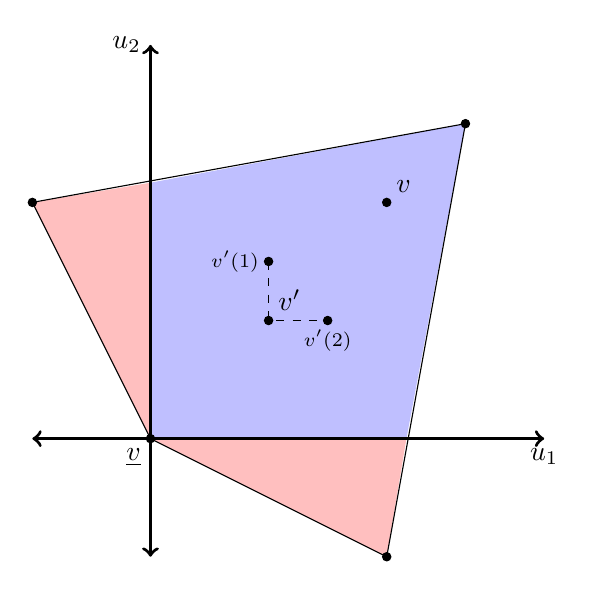
\begin{tikzpicture}[scale=0.5]
			\fill[blue, nearly transparent] (0,0)--(0,6.5)--(8,8)--(6.5,0)--(0,0);
			\fill[red, nearly transparent] (0,0)--(0,6.5)--(-3,6)--(0,0);
			\fill[red, nearly transparent] (0,0)--(6.5,0)--(6,-3)--(0,0);
			\draw[<->,very thick] (0,10)--(0,0)--(10,0);
			\draw[<->,very thick] (0,-3)--(0,0)--(-3,0);
			\node[below] at (10,0) {$u_1$};
			\node[left] at (0,10) {$u_2$};
			\filldraw (0,0) circle(3pt);
			\filldraw (-3,6) circle(3pt);
			\filldraw (8,8) circle(3pt);
			\filldraw (6,-3) circle(3pt);
			\filldraw (3,3) circle(3pt);
			\filldraw (6,6) circle(3pt);
			\filldraw (3,4.5) circle(3pt);
			\filldraw (4.5,3) circle(3pt);
			\node[above right] at (6,6) {$v$};
			\node[above right] at (3,3) {$v'$};
			\node[left] at (3,4.5) {\scriptsize $v'(1)$};
			\node[below] at (4.5,3) {\scriptsize $v'(2)$};
			\draw[dashed] (3,4.5)--(3,3)--(4.5,3);
			\draw (0,0)--(-3,6)--(8,8)--(6,-3)--(0,0);
			\node[below left] at (0,0) {$\underline{v}$};
		\end{tikzpicture}
	\end{figure}
	
	Assume further that there exists $a^i$ such that $g(a^i) = v'(i)$. Assume that there is a pure strategy profile $m^i$ that minimaxes $i$, so $g_i(m^i) = \underline{v}_i$. We will return to this assumption later. We now construct the following \emph{carrot and stick} strategies:
	\begin{itemize}
		\item Stage I: Play $a$ as long as nobody deviates. If $j$ alone deviates, go to II$_j$ (if two or more deviate, stay in I)
		\item Stage II$_j$: Play $m^j$ for $N$ periods, then go to III$_j$ if nobody deviates. If $k$ deviates, restart as II$_k$.
		\item Stage III$_j$: Play $a^j$ as long as nobody deviates. If $k$ alone deviates, go to II$_k$.
	\end{itemize}
	To check that these are optimal, we check every subgame in turn (for player $i$)
	
	In subgame I, if $i$ follows the strategy they get $v_i$, if they deviate they get \[(1-\delta) (\max_a g_i(a) + \delta \underline{v}_i + \cdots + \delta^N \underline{v}_i + \delta^{N+1} v_i' + \cdots)\]where deviation is obviously lower for sufficiently large $\delta$ since $\underline{v}_i < v'_i < v_i$.
	
	In subgame II$_i$, suppose that there are $N' \le N$ periods left. If $I$ follows the strategy, they get \[(1-\delta^{N'}) g_i(m^i) + \delta^{N'}v_i' = q(N') = (1-\delta)g_i(m^i) + \delta q(N'-1)\]where $g_i(m^i)$ is the payoff at the minimax strategy $m^i$ for $i$. If $i$ deviates, they do not improve in the deviating period and the punishment stage is restarted. So deviating attains
	\[(1-\delta)g_i(m^i) + \delta q(N) < (1-\delta)g_i(m^i) + \delta q(N'-1)\]
	
	In subgame II$_j$, suppose that there are $N' \le N$ periods left. If $i$ follows the strategy, they get
	\[
	(1-\delta^{N'})g_i(m^j) + \delta^{N'}(v_i' + \varepsilon)
	\]and if they deviate, they get \[(1-\delta)\max_a g_i(a,m_{-i}^j) + \delta (1-\delta^N)\underline{v}_i + \delta^{N+1} v_i'\]which is clearly strictly less.
	
	Finally, in subgame III$_i$, if $i$ follows the strategy, they get $v_i'$, and if they deviate they get \[(1-\delta) \max_a g_i(a,a^i_{-i}) + \delta (1-\delta^N)\underline{v}_i + \delta^{N+1}v_i'\]but this is strictly less since we assumed that $N$ was such that $\max_a g_i(a) + N\underline{v}_i < \min_a g_i(a) + Nv'_i$.
\end{proof}

\begin{remark}
	At two steps, we assumed that pure action profiles existed to generate the utilities we need. We could generate this if we had public randomizations, or by constructing strategies that change over time.
\end{remark}
\begin{remark}
	We also assumed (further) that the minimax strategy could be implemented with a pure strategy. If this is not the case, we need to ensure that players are willing to use a mixed minimax strategy. To this goal, a player $i$ must be willing to mix over a set of actions. This is possible only if the player is indifferent among the actions. This is possible, by changing around the exact values of $\varepsilon$. However, it complicates the proof considerably.
\end{remark}
\begin{remark}
	The assumption here is that $\dim V\opt = I$. We could weaken this to no player having payoffs that are an affine transformation of another player's payoffs. A certain qualification on payoffs is, however, necessary. Consider the following game, where $P1$ selects rows, $P2$ selects columns, and $P3$ selects the matrix:
	\begin{center}
	\begin{tabular}{c|cc}
		& $A$ & $B$ \\\hline 
		$A$ & $(1,1,1)$ & $(0,0,0)$ \\
		$B$ & $(0,0,0)$ & $(0,0,0)$ 
	\end{tabular}
	\qquad \qquad \qquad
	\begin{tabular}{c|cc}
		& $A$ & $B$ \\\hline 
		$A$ & $(0,0,0)$ & $(0,0,0)$ \\
		$B$ & $(0,0,0)$ & $(1,1,1)$ 
	\end{tabular}
	\end{center}
	\[A \qquad\qquad\qquad\qquad\qquad\qquad\qquad\qquad\qquad B\]
	Visually, this is Figure~\ref{fig:folk_counter}.
	\begin{figure}[H]
		\centering
			\begin{tikzpicture}[x={(0.866cm,-0.5cm)}, y={(0.866cm,0.5cm)}, z={(0cm,1cm)}]
			\coordinate (O) at (0,0,0);
			\coordinate (A) at (1,0,0);
			\coordinate (B) at (1,1,0);
			\coordinate (C) at (0,1,0);
			\coordinate (D) at (0,0,1);
			\coordinate (E) at (1,0,1);
			\coordinate (F) at (1,1,1);
			\coordinate (G) at (0,1,1);

			\draw[-stealth] (O) -- (4,0,0) node[right] {$x$};
			\draw[-stealth] (O) -- (0,4,0) node[above] {$y$};
			\draw[-stealth] (O) -- (0,0,4) node[above] {$z$};

			\draw[dashed] (O) -- (A) -- (B) -- (C) -- cycle;
			\draw[dashed] (D) -- (E) -- (F) -- (G) -- cycle;
			\draw[dashed] (O) -- (D);
			\draw[dashed] (A) -- (E);
			\draw[dashed] (B) -- (F);
			\draw[dashed] (C) -- (G);

			\draw[magenta, very thick] (O) -- (F);

			\fill (O) circle (1.5pt);
			\fill[magenta] (F) circle (1.5pt);
			\node[right] at (F) {$(1,1,1)$};


		\end{tikzpicture}
		\caption{Folk Counterexample}
		\label{fig:folk_counter}
	\end{figure}

	In this game, the minimax is 0 for all players, and the set of feasible individually rational payoffs is $V\opt = \{(v,v,v) : v \in (0,1)\}$ (on the plot in \textcolor{magenta}{magenta}). Can we get all of these as SPE? No! Let
	\[\underline{v} = \inf\{v : (v,v,v) \text{ is a SPE payoff} \}\]
	For $v$ to be a SPE we need that $v \ge \frac{1}{4}(1-\delta) + \delta \underline{v}$ since there must be at least two players in the three with $s_i(A) \ge 1/2$ or $s_i(B) \ge 1/2$ in the first period. Say that $s_1(A) \ge 1/2$ or $s_1(B) \ge 1/2$. Then $\underline{v} \ge \frac{1}{4}(1-\delta + \delta \underline{v} \Longleftrightarrow \underline{v} \ge \frac{1}{4}$ since 3 can choose $A$ in the first period. Therefore, there is no SPE with payoffs, say, $(1/8,1/8,1/8)$. 
\end{remark}



\subsection{Imperfect Public Monitoring}

A limitation of the repeated games model studied so far is that we assume that actions are observable. In many interesting applications, this is not the case. Imagine a case where actions are unobservable, but there are \blue{imperfect public signals} correlated to the actions. These signals can be used in a repeated game to sustain cooperation (or more generally as inputs to a player's strategies). 


\begin{model}\red{Imperfect Public Signals}
	Let $(A_1,\dots,A_I)$ be finite actions sets, and let $Y$ be a finite set of public outcomes. Let $\pi(y\mid a) = \prob(y\mid a)$. Let $r_i(a_i,y)$ be $i$'s payoff if she plays $a_i$ and the public outcome is $y$. Player $i$'s expected payoff is \[g_i(a) = \sum_{y\in Y} \pi(y\mid a) \cdot r_i(a_i,y)\]A mixed strategy is $\alpha_i \in \Delta(A_i)$. Payoffs are defined the obvious way. The \blue{public information} at the start of period $t$ is $h^t = (y^0,\dots,y^{t-1})$, and the \blue{private information} for player $i$ in period $t$ $h_i^t$ is her sequence of past actions. A strategy for $i$ is a sequence of maps $\sigma_i^t: (h^t,h^t_i) \to \Delta(A_i)$. 
	
	\begin{definition}
		A \blue{public strategy} for player $i$ is a sequence of maps $\sigma^t_i:h^t \to \Delta(A_i)$. 
	\end{definition}
	We focus on public strategies because they are simple and lead to a nice structure for the game.\footnote{This is just a refinement of the equilibrium concept -- an equilibrium in public strategies is still a Nash equilibrium.} Player $i$'s average discounted payoff for the game if she gets a sequence of payoffs $\{g_i^t\}$ is \[(1-\delta) \expect_\sigma \sum_{t=0}^\infty \delta^t g_i(\sigma(h^t))\]
	
	\begin{definition}
		A profile $(\sigma_1,\dots,\sigma_I)$ is a \blue{perfect public equilibrium (PPE)} if: (i) $\sigma_i$ is a public strategy for all $i$, and (ii) for each date $t$ and \emph{public} history $h^t$, the strategy is a Nash equilibrium starting from that point.
	\end{definition}
	\begin{remark}
		A player might be uncertain to which node they are at -- since we have \emph{imperfect} public information, officially this is distinct from SPE (and SPE has no bite here). However, since opponents don't use private information in their own strategies, all possible nodes have the same distribution over opponent play, so there's no need to distinguish. Like the set of subgame perfect equilibrium payoffs in a repeated game model with perfect monitoring, the set of PPE payoffs is stationary.
	\end{remark}
\end{model}

A special case of public monitoring is when $Y=A$, and $\pi(y \mid a) = 1$. In that case, all PPE are SPE and vie versa. Note that PPE are perfect Bayesian equilibria of the repeated game, but not all perfect Bayesian equilibria are PPE.

\begin{example}
	\red{Canonical Example} (from \href{https://www.jstor.org/stable/1911462?seq=1}{Green \& Porter, 1984}) Actions are interpreted as quantities, $a_i = q_i \in [0,Q]$, where quantities are unobserved. They determine an observed marker price $p = P(q,\varepsilon)$, where $p$ is a random variable: $\lambda(q) = \prob\{p \ge \hat{p}\mid q\}$. Green and Porter study collusion, an equilibrium in \blue{trigger price strategies}. In Phase I, we produce $\hat{q}$. If $p \ge \hat{p}$, stay in this phase. If not, go to Phase II, where we play a static equilibrium for $T$ periods. The value for these strategies in Phase I is:
	\[
	\hat{v} = (1-\delta)g(\hat{q}) + \delta\barl \lambda(\hat{q}) + (1-\lambda(\hat{q}))\delta^T \barr\hat{v} \Longleftrightarrow \hat{v} = \frac{(1-\delta)g(\hat{q})}{1-\delta \barl \lambda(\hat{q}) + (1-\lambda(\hat{q}))\delta^T \barr}
	\]
	where we normalize the payoff of the punishment phase to zero. Obviously in Phase II, the static equilibrium is incentive compatible. In Phase I, we need that \[(1-\delta)g(q_i,\hat{q}_{-i}) + \delta \barl \lambda(q_i,\hat{q}_{-i}) + (1-\lambda(q_i,\hat{q}_{-i}))\delta^T\barr \hat{v} \le \hat{v}\]It can be shown that there exist parameters under which these equilibria are attainable. A hypothetical designer designing a collusive equilibrium would choose $\hat{q}, \hat{p}, T$ to maximize $\hat{v}$ subject to the strategies being an equilibrium.
\end{example}

\begin{model}
	\red{Dynamic Programming} (from \href{https://www.sciencedirect.com/science/article/pii/0022053186900281}{Abreu, Pearce, \& Stochetti, 1986} and \href{https://www.jstor.org/stable/2938299?seq=1}{1990}) \begin{definition}
		A pair $(\alpha,v)$ is \blue{enforceable} with respect to $\delta$ and $W \subseteq \reals^I$ if there exists a function $w: Y \to W$ such that for all $i$,\[v_i = (1-\delta)g_i(\alpha) + \delta \sum_{y\in Y} \pi(y \mid \alpha)\cdot  w_i(y)\]and \[\alpha_i \in \argmax_{\alpha_i' \in \Delta(A_i)} \barl (1-\delta)g_i(\alpha_i',\alpha_{-i}) + \delta \sum_{y \in Y} \pi(y \mid \alpha_i',\alpha_{-i}) \cdot w_i(y)\barr\]
	\end{definition}
	\begin{remark}
		The first condition says that the target payoff $v$ can be decomposed into today's payoff and the expected continuation payoff, and that the strategy maximizes that decomposed value function. The second condition is incentive compatibility.
	\end{remark}
	These conditions are similar to Bellman's Equation.
	
	\begin{definition}
		Let $B(\delta,W)$ be the set of payoffs $v$ such that for some $\alpha$, $(\alpha,v)$ is enforced with respect to $\delta$ and $W$. Then $B(\delta,W)$ is the payoff set \blue{generated} by $\delta,W$.
	\end{definition}
	\begin{definition}
		Let $E(\delta)$ be the set of \blue{PPE payoffs} 
	\end{definition}
	\begin{proposition}
		$E(\delta) = B(\delta,E(\delta))$
	\end{proposition}
	\begin{proof}
		$(\supseteq)$: Fix $v \in B(\delta,E(\delta))$. Pick $w : Y \to E(\delta)$ such that $w$ enforces $(\alpha,v)$. Now consider the following strategies: In period 0, play $\alpha$. Then starting in period 1, play the perfect public equilibrium that gives payoffs $w(y_0)$. This is a PPE, so $v \in E(\delta)$.
		
		$(\subseteq)$: If $v \in E(\delta)$, then there exists a PPE that gives	$v$ as payoffs. Suppose in this PPE, play in period 0 is $\alpha$, and continuation payoffs are $w(y_0) \in E(\delta)$, since continuation corresponds to PPE play. The fact that nobody wants to deviate means that $(\alpha,v)$ is enforced by $w$, so $v \in B(\delta,E(\delta))$.
	\end{proof}
		
	Abreu, Pearce, and Stacchetti call this \blue{factorization}. If it is possible to sustain average payoffs in $W$ by promising different continuation payoffs in $W$, then $W$ is self-generating. Formally,
	\begin{definition}
		$W$ is \blue{self-generating} if $W \subseteq B(\delta,W)$.
	\end{definition}
	\begin{remark}
		Note that $E(\delta)$ is self-generating. The set of static Nash equilibrium payoffs is also self-generating.
	\end{remark}
	\begin{proposition}
		If $W$ is self-generating, then $W \in E(\delta)$.
	\end{proposition}
	\begin{proof}
		Fix $v \in W$. Then $v \in B(\delta,W)$ so there is some $w :Y\to W$ and some $\alpha$ such that $(\alpha,v)$ is enforced by $w$. We will construct an equilibrium that gives $v$. In period 0, play $\alpha$, and for an outcome $y_0$ set $v_1 = w(y_0)$. Then $v_1 \in W \subseteq B(\delta,W)$, so again there is some $\alpha_1$ and some $w_1: Y \to W$ such that $(\alpha_1,v_1)$ is enforced by $w_1$. Continue this strategy forever, to obtain the recommended strategies. After each public history there are no profitable deviations, and by construction the payoff is $v$.
	\end{proof}
	\begin{corollary}
		$E(\delta)$ is the largest self-generating set.
	\end{corollary}
\end{model}


\begin{example}
	\red{Prisoner's Dilemma with Perfect Monitoring} We noted that games with perfect monitoring are special examples of games with public information, so we can think of the strategies above here. Let $Y = \{(C,C),(C,D),(D,C),(D,D)\}$. We will show that for $\delta \ge \frac{1}{2}$, the set $W = \{(0,0),(1,1)\}$ is self-generating. To this, we show that $(0,0), (1,1) \in B(\delta,W)$ for $\delta \ge \frac{1}{2}$. Seeing that $(0,0) \in B(\delta,W)$ is trivial, since it is the static Nash outcome. In fact, for any $\delta$ and $a_i$ we have that\[0 \ge (1-\delta) g_i(a_i,D) + \delta w_i(a_i,D)\]Now consider $(1,1)$. We will show that the strategy profile $(C,C)$ and payoff profile $(1,1)$ are enforced by $\delta \ge \frac{1}{2}$ and $W$. Let $w(C,C) = (1,1)$ and $w(y) = (0,0)$ for all $y \ne (C,C)$. Then \[1= (1-\delta) g_i(C,C) + \delta w_i(C,C) \]and for any $a_i$ and $\delta \ge \frac{1}{2}$,\[1 \ge (1-\delta)g_i(a_i,C) + \delta w_i(a_i,C)\]So $W \subseteq B(\delta,W)$ for $\delta \ge \frac{1}{2}$, meaning that $W$ is self-generating.
	
\end{example}



\begin{example}
	\red{Another PD Example} Consider this game:
	\begin{center}
		\begin{tabular}{c|cc}
			& $C$ & $D$ \\\hline 
			$C$ & $(2,2)$ & $(-1,3)$ \\
			$D$ & $(3,-1)$ & $(0,0)$
		\end{tabular}
	\end{center}
	Again assume that $Y = \{(C,C),(C,D),(D,C),(D,D)\}$. We now intend to prove that if $\delta \ge 1/3$, then $W = \{v,\hat{v}\}$ is self-generations, where \[v = \parl \frac{3-\delta}{1+\delta}, \frac{3\delta - 1}{1+\delta} \parr \qquad \text{ and } \qquad \hat{v} = \parl \frac{3\delta - 1}{1+\delta}, \frac{3-\delta}{1+\delta}\parr\]Since it is a symmetric game and the continuations in $W$ are permutations, we need only to show that $v$ can be enforced with continuation in $W$. 
	
	Let the action profile $\alpha$ corresponding to $v$ be $(D,C)$ and the continuation payoffs be $w(D,C) = w(C,C) = \hat{v}$ and $w(D,D) = w(C,D) = v$. If players follow $\alpha$, then the payoffs are \[(1-\delta) \cdot \matrixp{3 & -1} + \delta\cdot  \hat{v} = \parl \frac{3(1-\delta^2+3\delta^2 -\delta)}{1+\delta}, -\frac{(1-\delta^2) + 3\delta - \delta^2}{1+\delta}\parr = v\]Clearly $D$ maximizes the first player's action, since the current action does not affect future payoffs. If player 2 plays $C$ as required by $\alpha$, then they attain payoff $v_2 = \frac{3\delta-1}{1+\delta}$. If player 2 plays $D$, the payoff is 0 today and $v_2$ tomorrow. Thus, playing $C$ is optimal as long as $v_2 \ge 0 \Longleftrightarrow \delta \ge \frac{1}{3}$.
\end{example}

\begin{remark}
	Recall that Folk Theorems aim to prove that all feasible and individually rational payoffs (\ie $V\opt$) are achievable in equilibrium. A reasonable approximation is that any closed subset of $V\opt$ is achievable in equilibrium. Can we prove this statement with imperfect public monitoring?
	
	If nothing is observed, then only the static Nash payoffs are attainable. It is reasonable to assume that the signal structure is sufficiently rich to provide incentives using expected payoffs.
\end{remark}	
	Define $\pi(a_i \mid \alpha_{-i})$ to be a vector of probabilities on $Y$ generated by $a_i$ given $\alpha_{-i}$, so it is a $|Y|$-dimensional vector. Define $\Pi(\alpha_{-i})$ to be the $|A_i| \times |Y|$-dimensional matrix that stacks the $\pi(a_i\mid \alpha_{-i})$. If we ignore feasibility constraints, we can implement a utility vector $k$ as long as we can solve the system\[(1-\delta)G(\alpha_{-i}) + \delta \Pi_i(\alpha_{-i})w_i = k\]where $G_i(\alpha_{-i})$ is a column vector with generic element $g_i(a_i \mid \alpha_{-i})$ for all $a_i\in A_i$. The above system is solvable in $w_i$ if $\Pi_i(\alpha_{-i})$ is full-rank.

\begin{lemma}\label{lem:indiv_full_rank}
	The \blue{individual full rank condition} is satisfied by a profile $\alpha$ if for each player $i$, $\Pi_i(\alpha_{-i})$ is invertible, meaning that the vectors $\pi_i(a_i \mid \alpha_{-i})$ are linearly independent.
\end{lemma}

\begin{remark}
	The individual full rank condition is not sufficient for a Folk Theorem. Consider the following example, from \href{https://www.jstor.org/stable/2297591}{Radner, Myerson, \& Maskin (1986)}. Two players can either work or shirk, at costs of 1 and 0 respectively. Output can be high or low, with probabilities from each outcome. If output is high, both players receive 4, otherwise they receive 0. The probability of high output is:\[\pi_H(W,W) = \frac{9}{16} \qquad ; \qquad \pi_H(W,S) = \pi_H(S,W) = \frac{3}{8} \qquad ; \qquad \pi_H(S,S) = \frac{1}{4}\]The individual full rank condition is satisfied at $\alpha = (W,W)$, since \[\Pi_i(\alpha_{-i}) = \matrixc{\pi_H(W,W) & 1 - \pi_H(W,W) \\ \pi_H(S,W) & 1-\pi_H(S,W)} = \underbrace{\matrixc{ 9/16 & 7/16 \\ 3/8 & 5/8}}_{\text{Full Rank}}\] Despite the fact that the individual full rank condition holds, the Folk Theorem does not. To see this, let $v\opt$ be the highest payoff in any symmetric equilibrium. If the Folk Theorem is true, we should be able to get a payoff close to $4 \cdot \frac{9}{16} - 1 = \frac{5}{4} > 1$, since if the players choose $(H,H)$, expected payoff is $(5/4,5/4)$. We show that these payoffs cannot be approximated (in pure strategies only. The proof for mixed strategies follows fairly easily).
	
	If the theorem holds, $v\opt > 1$, and since the equilibrium is stationary in equilibrium the players must choose $(H,H)$ with at least positive probability. So we have that \[v\opt = (1-\delta) \barl \frac{9}{16} \cdot (4 + \delta \cdot v_g) + \frac{7}{16} \cdot (0 + \delta \cdot v_b) - 1\barr \ge (1-\delta) \barl \frac{3}{8} \cdot (4 + \delta \cdot v_g) + \frac{5}{8} \cdot (0 + \delta \cdot v_b) - 1\barr\]which implies that $v_g - v_b \ge \frac{4}{3}\cdot \frac{1-\delta}{\delta}$. However, by definition $v\opt \ge v_g$, so \[v\opt \le (1-\delta)\frac{5}{4}+ \delta \barl \frac{9}{16} \cdot v\opt + \frac{7}{16} \cdot \parl v\opt - \frac{4}{3} \cdot \frac{1-\delta}{\delta}\parr \barr \Longleftrightarrow v\opt \le \frac{3}{2} \le 1 \Rightarrow \! \Leftarrow\]
	From this example, we learn that we need an additional assumption.
 \end{remark}
 
 Define the matrix $\Pi_{i,j}(\alpha)$ to be the matrix formed by vertically concatenating the matrices $\Pi_i(\alpha_{-i})$ and $\Pi_j(\alpha_{-j})$. It is a $\parl |A_i| + |A_j|\parr \times |Y|$-matrix.
 
 \begin{lemma}\label{lem:pairwise_full_rank}
 	The \blue{pairwise full-rank condition} is satisfied at action $\alpha$ for players $i$ and $j$ if $\Pi_{i,j}(\alpha)$ has maximal rank (equivalent to full column rank). 
 \end{lemma}
 
 Note that $\Pi_{i,j}(\alpha)$ cannot have full row rank, so the $|A_i| + |A_j|$ vectors admit at least one linear dependency. To see this, note that \[\pi(\alpha) = \sum_{a_i\in A_i}\alpha_i(a_i) \cdot \pi(a_i \mid \alpha_{-i}) = \sum_{a_j\in A_j}\alpha_j(a_j) \cdot \pi(a_j \mid \alpha_{-j})\]So we have that \[\pi(a_1\mid \alpha_{-i}) = \sum_{a_j\in A_j}\frac{\alpha_j(a_j)}{\alpha_1(a_1)} \cdot \pi(a_j \mid \alpha_{-j}) - \sum_{a_i\in A_i}\frac{\alpha_i(a_i)}{\alpha_1(a_1)} \cdot \pi(a_i \mid \alpha_{-i})\]which is the linear dependency. Thus, we have:
 
 \begin{proposition}
 	\red{Imperfect Public Monitoring Folk Theorem} Suppose that $\dim V = I$, and both the individual full-rank condition (Lemma~\ref{lem:indiv_full_rank}) and the pairwise full-rank condition (Lemma~\ref{lem:pairwise_full_rank}) hold. Then for any closed set $W \subset \int(V\opt)$, there exists some $\delta\opt < 1$ such that for any $\delta \ge \delta\opt$, $W \subset E(\delta)$.
 \end{proposition}
\begin{remark}
	Some limitations exist here. A necessary condition to satisfy Lemma~\ref{lem:pairwise_full_rank} is that $|A_i| + |A_j| - 1 \le |Y|$, which may be demanding. Indeed, it is not satisfied in the earlier Radner, Myerson, \& Maskin example, in which we have two signals but $|A_i| + |A_j| - 1 = 3$. Moreover, the signal structure needs to be rich enough. For example, even if we have more than two signals it fails at symmetric profiles (\ie $(W,W)$):
	\[
	\Pi_{ij}(\alpha)  = \matrixc{\pi_H(W,W) \\\pi_H(S,W) \\\pi_H(W,W) \\\pi_H(W,S)}
	\]
	where $\pi_H(W,W)$ has $|Y|$ dimensions. This matrix has rank $2 < 3$, since $\pi_H(L,H) = \pi_H(H,L)$. 
\end{remark}


\subsection{Imperfect Private Monitoring}

\begin{example}
	Consider the following simply two-player game. In the first period, the players play a standard Prisoner's Dilemma (with payoffs $(1,1), (2,-1), (-1,2), (0,0)$). In the second period, they play the coordination game 
	\begin{center}
		\begin{tabular}{c|cc}
			& $G$ & $B$ \\\hline
			$G$ & $(k,k)$ & $(0,0)$ \\
			$B$ & $(0,0)$ & $(1,1)$
		\end{tabular}
	\end{center}
	with $k > 2$. We can use the multiplicity of equilibria in the second game to incentivize cooperation in the first period. In perfect monitoring, the obvious strategy to cooperate, and play $G$ if both cooperate, sustains cooperation for sufficiently large $\delta$.
	
	Now suppose that the first-period actions $(a_1,a_2)$ are not observed. Rather, each player $i$ observes a signal $y_i \in \{c,d\}$ about her opponent's action. Suppose that \[\prob\{y_i = c \mid a_j\} = \begin{cases} 1 - \varepsilon & a_j = C \\ \varepsilon & a_j = D\end{cases}\]where if $\varepsilon$ is small, monitoring is almost perfect. We would expect that when $\varepsilon$ is arbitrarily small, we could obtain cooperation. However, even for extremely small but positive $\varepsilon$, no pure strategy equilibrium where the players cooperate in period 1 can be sustained.
	
	Observe that in the second period, $i$ will want to play $G$ if and only if she assigns probability $\frac{1}{k+1}$ or greater to the other player playing $G$. Consider strategies that call for each player to play $C$ in the first period and $G$ in the second if and only if $y_i = c$. If $i$ plays $C$ in the first period, she assigns probability $1-\varepsilon$ to $j$ observing $c$ and hence to $j$ playing $G$. However, regardless of what signal she observes she will want to play $G$, so won't want to follow the strategy. 
	
	\begin{remark}
		Note that $i$ and $j$'s are \emph{conditionally independent}. So long as $i$ cooperates in the first period, she will assign high probability to $j$ observing a good signal regardless of her own signal. This means that she prefers to keep cooperating no matter what. Essentially, private monitoring means that there is no way to coordinate on the punishment outcome following a bad outcome and on the good equilibrium otherwise, so there can be no enforcement.
	\end{remark}
	
	The coordination problem is removed if the players' signals are correlated rather than independent. Let's consider the extreme case of perfect correlation: Suppose for simplicity that $y_j = y_i = y \in \{c,d\}$, where \[\prob\{y_1 = y_2 = c \mid (a_1,a_2)\} = \begin{cases}1-\varepsilon & a_1=a_2=C \\ \varepsilon & \text{otherwise} \end{cases}\]Consider strategies that call for each player to play $C$ in the first period, and $G$ in the second period if and only if they observe $c$. This clearly gives an equilibrium in the second period, and checking first period incentives we have that \begin{align*} u(C) &= 1 + (1-\varepsilon)(k-1) + 1 \\ u(D) &= 2 + \varepsilon(k-1) + 1 \end{align*}so it is optimal to play $C$ for $k \ge 1 + \frac{1}{1-2\varepsilon}$, which is ensured for $\varepsilon$ sufficiently small. 
	
	More generally, if $y_i$ and $y_j$ are correlated but not perfectly correlated, we may still be able to sustain cooperation in the first period by coordinating on different second period play depending on the signals. Because signals are correlated at $t=2$, they self-enforce. What we really have now is a game with \blue{imperfect public monitoring}.
\end{example}

\begin{remark}
	Even if the private signals are independent, players may be able to correlate their beliefs by playing mixed strategies in the first period. Returning to the independent signals, consider the following strategies: In period 1, player $i$ plays $C$ with probability $\alpha \in (0,1)$. In period 2, player $i$ plays $G$ if and only if $a_i = C$ and $y_i = c$. In the second period, $i$ will want to play $G$ if and only if she assigns probability $\frac{1}{k+1}$ or greater to $j$ playing $G$. She assigns this probability by conditioning on what she knows: her action $a_i$ and her signal $y_i$. \[\prob\{a_2^j = G \mid a_i,y_i\} = \prob\{y_j = c \mid a_i\} \cdot \prob\{a_j = C \mid y_i\}\]Which holds because of independence and the assumption that $j$ is playing the same strategy. Bayes' Rule gives the probabilities \[ \begin{array}{c|c} a_i,y_i & \prob\{a_2^j = G \mid a_i,y_i\} \\\hline \\ C,c & (1-\varepsilon) \frac{(1-\varepsilon)\alpha}{(1-\varepsilon)\alpha + \varepsilon(1-\alpha)} \\\\ C,d & (1-\varepsilon) \frac{\varepsilon\alpha}{\varepsilon\alpha + (1-\varepsilon)(1-\alpha)} \\\\ D,c & \varepsilon \frac{(1-\varepsilon)\alpha}{(1-\varepsilon)\alpha + \varepsilon(1-\alpha)} \\\\ D,d & \varepsilon \frac{\varepsilon\alpha}{\varepsilon\alpha + (1-\varepsilon)(1-\alpha)} \end{array}\]Aside from the $(C,c)$ case, the probability that $j$ will play $G$ is of order $\varepsilon$, so for sufficiently small $\varepsilon$, $i$ will be willing to follow the prescribed strategy in the second period. Now consider $i$'s incentives in the first period. Her expected payoffs for each strategy are: \begin{align*} u_i(C) &= \alpha \barl a + (1-\varepsilon)^2 k + (1-\varepsilon)\varepsilon \cdot 0 + (1-\varepsilon)\varepsilon \cdot 0 + \varepsilon^2 \cdot 1\barr + (1-\alpha)\barl -1 + (1-\varepsilon) \cdot 1 + \varepsilon\cdot 0\barr \\ &= \alpha (1+\varepsilon^2) - (1-\alpha) + (1-\varepsilon)^2 \barl \alpha k + (1-\alpha)\barr \approx \alpha (1+k) \\ u_i(D) &= \alpha (2 + \varepsilon \cdot 0 + (1-\varepsilon) \cdot 1) + (1-\alpha) [0 + 1] \\ &= 2\alpha + 1 - \varepsilon\alpha \approx 2\alpha + 1\end{align*}We can make $i$ indifferent between $C$ and $D$ by setting $\alpha \to \frac{1}{k-1}$ as $\varepsilon \to 0$. Note that the key to a mixed equilibrium is that player $i$ conditions his second period behavior on the result of his first period randomization. Because of this, player $j$'s signal is now informative about $i$'s second period behavior. This means that $j$ will want to condition their second period action on the first period signal, which means i turn that there are incentives to cooperate in the first period. 
\end{remark}

\begin{remark}
	The problem with imperfect private independent monitoring is that with pure strategies and signals with full support, there is no Bayesian updating as low signals are attributed to chance. This would not happen if the players played mixed strategies, correlated with the state in which the players are.
\end{remark}

There is a lovely construction of a folk theorem with private monitoring, from \href{https://www.sciencedirect.com/science/article/pii/S0022053100927741?ref=pdf_download&fr=RR-2&rr=922d8a14ed957d16}{Ely \& Valimaki (2002)}. They show it only for the Prisoner's Dilemma, but it easily extends.

\begin{theorem}
	\red{Robust Folk Theorem with Private Monitoring} Let $(v_1,v_2) \in V^\circ$. There exist $\bar{\delta},\varepsilon \in (0,1)$ such that for all $\delta \in (\bar{\delta},1)$ and for all $\varepsilon$-perfect monitoring technologies $m$, there exists a sequential equilibrium of $G^\infty(\delta,m)$ with payoffs $(v_1,v_2)$.
\end{theorem}
\begin{proof}
	(Intuitive, by construction). The idea is to construct an equilibrium in which the players are indifferent between $C$ and $D$ at every point in time. Consider the standard Prisoner's Dilemma and assume that player $i$ observes a signal $y_i \in \{c,d\}$ correlated to $j$'s action, where \[\prob\{y_i = c\} = \begin{cases} 1- \varepsilon & a_j = C \\ \varepsilon & a_j = D\end{cases}\]To get a sense of the construction, first consider the case with perfect monitoring. Construct a state contingent mixed strategy in which $\varphi_{a_i,y_i}^i$ is the probability of selecting $C$ in state $a_i,y_i$. We will construct an equilibrium in which (1) when $j$ selects $C$ at $t$, $i$ is indifferent between $C$ and $D$ and receives $V^i_C$; and (2) when $j$ selects $D$ at $t$, $i$ is indifferent between $C$ and $D$ and receives $V^i_D$. We have value functions: \begin{align*} V_C^i &= (1-\delta) + \delta\barl \phi^j_{C,C} V^i_C + (1-\phi^j_{C,C}) V^i_D\barr \\ V_C^i &= 2(1-\delta) + \delta \barl \phi^j_{C,D} V^i_C + (1-\phi^j_{C,D})V^i_D\barr \\ V_D^i &= -(1-\delta) + \delta \barl \phi^j_{D,C} V^i_C + (1-\phi^j_{D,C})V^i_D\barr \\ V_D^i &= 0 \cdot (1-\delta) + \delta \barl \phi^j_{D,D} V^i_C + (1-\phi^j_{D,D})V^i_D\barr\end{align*}Proof follows by showing that for any $V_C^i,V_D^i$ where $1 \ge V_C^i \ge V_D^i \ge 0$, we can achieve it in equilibrium for $\delta$ sufficiently close to 1. This allows us to obtain any pair $(v_1,v_2) \in V$.
\end{proof}

\begin{remark}
	This construction can be generalized to imperfect monitoring, where $\varepsilon > 0$ (but small). This gives a lot of equilibria but is not yet sufficient for a Folk Theorem. To do this, we add a preliminary phase of finite length, and we support different payoffs in the preliminary phase with different continuation payoffs in the unit square. This gives us a true Folk Theorem in the case where monitoring is nearly perfect.
\end{remark}


\section{Bayesian Games}

\paragraph{Preliminaries.}

\begin{remark}
	In Bayesian Game we study interactions in which there may be uncertainty about the characteristics of the other players (or the state of nature). \blue{States of nature} are a description of the player's relevant characteristics!
\end{remark}

\begin{definition}
	A \blue{Bayesian game} consists of (i) a finite set $N$ of players; (ii) a finite set of states of nature $\Omega$ (finite here for simplicity); and (iii) for each $i \in N$, a set $A_i$ of actions, a finite set of types $T_i$ and a signal function $\tau_i : \Omega \to T_i$), a probability measure $p_i$ over $\Omega$ with $p_i(\tau_i^{-1}(t_i)) > 0$ for all $t_i \in T_i$, and a preference relation $\succeq_i$ over $A \times \Omega$. A Bayesian game is thus a tuple: $\langle N, \Omega, \{A_i\},\{T_i\},\{\tau_i\},\{p_i\},\{\succeq_i\}\rangle$.
\end{definition}

Often a Bayesian game is not defined in terms of $\Omega$ and the \blue{signal function} $\tau_i$ but directly in terms of types. Sometimes it is described in terms of $\Omega$ and a signal structure expressed as a conditional distribution over types $T_i$. In this case, we denote the conditional probability as $\tau_i(t_i;\omega)$. In the definition, we allow for heterogeneous priors on $\Omega$. Often it is assumed that there is a common prior.

\begin{definition}
	A \blue{Nash equilibrium of a Bayesian game} is the Nash equilibrium of a strategic game defined as follows: (i) the set of players is the set of pairs $(i,t_i)$ for each $i \in N$ and $t_i \in T_i$; (ii) the set of actions of player $(i,t_i)$ is $A_i$; and the preferences $\succeq_{i,t_i}$ are such that \[a\opt \succeq_{i,t_i} b\opt \Longleftrightarrow L_i(a\opt,t_i) \succeq_i L_i(b\opt,t_i)\]where $L_i(a\opt,t_i)$ is a lottery that assigns probability $\frac{p_i(\omega)}{p_i(\tau^{-1}(t_i))}$ to $\parl \{a\opt(j,\tau_j(\omega))\}_{j\in N},\omega\parr$ if $\omega \in \tau_i^{-1}(t_i)$ and 0 otherwise.
\end{definition}

\subsection{Applications}

\begin{example}
	\red{Collective Action} Consider a problem where a group of $n$ players can obtain a public good if at least one of them volunteers. The public good generates a value $v < 1$ to each player, and volunteering costs $c_i$ to player $i$. We assume $c_i \sim F(\cdot)$, with support $[0,\bar{c}]$, and we will focus on symmetric equilibria. In the formalism of above, we have states $(c_1,\dots,c_n) \in \Omega$, with signals $\tau_i : \Omega \to T_i$, where $\tau_i(c_1,\dots,c_n) = c_i$, and beliefs $\prob\{c_{-i} \mid c_i\} = \prod_{j \ne i} f(c_j)$. We also have linear utility, so $0$ if no contribution, $v$ if someone else contributes, and $v-c_i$ if you contribute. Assume that the probability of contribution for a player is $\sigma$. The expected utility of contributing is $u_i(C) = v - c_i$, and the expected utility of not contributing is $u_i(NC) = \prob\{a_j = C \text{ for at least } 1 j \ne i\} v$ Thus, the net utility of contributing is \[\Delta u_i = [1-\prob\{\# \text{volunteers } \ne i \ge 1\}] v - c_i = \prob\{\# \text{volunteers } \ne i = 0\}\cdot v - c_i\]if $\Delta u_i \ge 0$, then $\Delta u_j > 0$ if $c_j < c_i$. So there exists $c\opt$ such that a player $c_i$ volunteers if and only if $c_i \le c\opt$. What is $c\opt$? $c\opt = \prob\{\# \text{volunteers } = 0\}\cdot v = [1-F(c\opt)]^{n-1}v$. Note that this means that we have a unique equilibrium as long as the typical assumptions on $F(\cdot)$ hold. We can think about asymptotics here. Assume that $c_n\opt \to c\opt_\infty > 0$, then we have a contradiction. Thus, $c_n\opt \to 0$. However, the probability of success is \[P = 1-[1-F(c_n\opt)]^n = 1-\parl \frac{c_n\opt}{v}\parr^{\frac{n}{n-1}} \to 1\]
\end{example}

\begin{example}
	\red{Juries} Consider a trial in which $n$ jurors decided to acquit or convict a defendant. The defendant is guilty ($G$) with prior probability $\pi$ and innocent ($I$) otherwise. Each juror receives an informative signal $\{g,i\}$ with probability $\prob\{g \mid G\} =p > \frac{1}{2}$, and $\prob\{i \mid I\} = q > \frac{1}{2}$. The defendant is convicted if all jurors vote to convict. We assume that the voter's utility for a decision $x = (x_1,\dots,x_n)$ is\[u_i(x_i,x_{-i}) = \begin{cases} 0 & \text{if } x = c \& G \text{ or } x = a \& I \\ -z & \text{if } x = c \& I \\ -(1-z) & \text{if } x = a \& I\end{cases}\]Note that we can interpret $z$ as the belief threshold on the guilt of the defendant, such that below it acquitting is optimal. Indeed, if $r$ is the probability that a defendant is guilty (and $i$ is pivotal), then \begin{align*} u_i(a) &= -r(1-z) + (1-r) \cdot 0 \\ u_i(c) &= r \cdot 0 - (1-r)\cdot z\end{align*}So $a \succeq_i c \iff z \ge r$. Jurors face two types of costly mistakes: convicting an innocent and acquitting a guilty defendant. They need to assess the trade-off on the basis of all the information they have, so why is this a strategic situation? The outcome depends on the collective decision. The decision of a juror only matters if they're pivotal. The most simple case is when $n = 1$, since there are no strategic interactions. The posterior after an $i$ signal is \[\prob\{G \mid i\} = \frac{\prob\{i\mid G\} \cdot \prob\{G\}}{\prob\{i \mid G\}\cdot \prob\{G\} + \prob\{i \mid I \}\cdot (1-\prob\{G\})} = \frac{(1-p)\pi}{(1-p)\pi + q(1-\pi)}\]So a juror is willing to acquit after an innocent signal if and only if $z \ge \frac{(1-p)\pi}{(1-p)\pi + q(1-\pi)}$. Similarly, they are willing to convict after a guilty signal as long as $z \le \frac{p\pi}{p\pi +(1-q)(1-\pi)}$. Putting these together, a juror is willing to go with the signal if \[\frac{(1-p)\pi}{(1-p)\pi + q(1-\pi)} \le z \le \frac{p\pi}{p\pi +(1-q)(1-\pi)}\]It is not always the case that the signal determines the decision, because the signal may be weak compared with either the prior $\pi$ or the preferences $z$. Intuitively, some jurors will always convict and some will always acquit, if the inequalities above do not hold.
	
	With two jurors, the vote of a juror only matters if the other votes to convict. Can we have an equilibrium where both jurors vote according to their signal? In this case, the relevant posterior for $i$ is \[\prob\{G \mid i,g\} = \frac{(1-p)p\pi}{(1-p)p\pi + q(1-q)(1-\pi)}\]and following the logic above, an equilibrium exists only if \[\frac{(1-p)p\pi}{(1-p)p\pi + q(1-q)(1-\pi)} \le z \le \frac{p^2 \pi}{p^2\pi + (1-q)^2(1-\pi)}\] note that \[\frac{(1-p)p\pi }{(1-p)p\pi + q(1-q)(1-\pi)} > \frac{(1-p)\pi}{(1-p)\pi + q(1-\pi)}\]so the juror is more reluctant to vote to acquit. Intuitively, this comes from the fact that the juror assumes that the other juror is voting guilty when making their decision, so their posterior is shifted towards guilt.
	
	With $n$ jurors, the relevant posterior becomes \[\prob\{G; i,\{g\}_{-i}\} = \frac{\prob\{i,\{g\}_{-i};G\}\cdot \prob \{G\}}{\prob\{i,\{g\}_{-i};G\}\cdot \prob \{G\} + \prob\{i,\{g\}_{-i};I\}\cdot (1-\prob \{G\})} = \frac{(1-p)p^{n-1}\pi}{(1-p)p^{n-1}\pi + q(1-q)^{n-1}(1-\pi)}\]so a juror with signal $i$ acquits only if \[z \ge \frac{(1-p)p^{n-1}\pi}{(1-p)p^{n-1}\pi + q(1-q)^{n-1}(1-\pi)} = \frac{\pi}{\pi + \frac{q}{1-p} \parl \frac{1-q}{p}\parr^{n-1}(1-\pi)}\]As $n \to \infty$, the right hand side goes to 1, so for no $z < 1$ is the juror willing to follow their own signal. This means that for large $n$, we cannot have an equilibrium in which jurors follow signals with probability 1.
	
	\begin{remark}
		Under some conditions, there is an equilibrium in which the jurors \emph{partially} use the information from their signals. In these equilibria, the jurors with a $g$ signal vote to convict. The jurors with an $i$ signal vote to convict with probability $\sigma$. Then $\sigma$ is high, the informative content of the fact that $n-1$ other jurors vote to convict is sufficiently small that it does not dominate the jurors' private signals.
	\end{remark}
\end{example}





\subsection{Auctions}

\begin{definition}
	We have a \blue{seller} with an indivisible item for sale and zero cost. We have $I$ \blue{bidders} (players) indexed by $i = 1,\dots,I$, and each bidder $i$ has \blue{private information} $v_i \in V_i$. Given the profile $v = (v_i,v_{-i})$, bidder $i$'s \blue{valuation} is $u_i(v_i;v_{-i})$ if she gets the item and zero otherwise. The prior distribution over $V = \prod_i V_i$ is $F(v)$, and after knowing ones own $v_i$, bidder $i$ forms the posterior distribution of others' valuation payoff as $F_i(v_{-i};v_i)$. All bidders and sellers have quasilinear, von Neumann Morgenstern expected utility functions. A \blue{pure strategy} for bidder $i$ is $s_i \in S_i = [0,\infty)$, which admits \blue{winning probability} $P_i(s) = P_i(s_i,s_{-i})$ with \blue{monetary payment} $T_i(s_i,s_{-i})$. A model has \blue{private values} if $u_i(v_i,v_{-i}) = u_i(v_i,v'_{-i})$ for any $v_{-i}, v'_{-i}$, and a model has \blue{common values} otherwise. A model has \blue{independent values} if $f(v) = \prod_i f_i(v)$, and a model has \blue{symmetric values} if $f_i(v) = f(v)$.
\end{definition}

\begin{remark}
	From now on, we focus on the case with (i) independent, symmetric private values; and (ii) risk-neutral bidders, so \[\pi(v_i,s) = P_i(s_i,s_{-i})v_i - T_i(s_i,s_{-i})\]
\end{remark}

\begin{definition}
	A pure strategy in the typical case is a map $s_i\opt : V \to \reals_+$, and a strategy profile $(s_1\opt,\dots,s_I\opt)$ is an \blue{equilibrium in weakly undominated strategies} if \[\pi(s_i\opt(v_i);v_i,s_{-i}) \ge \pi(s_i;v_i,s_{-i}) \text{ for any } s_i,s_{-i}\]A strategy profilsis a \blue{Bayesian equilibrium} if \[\expect\barl \pi(s_i\opt(v_i);s\opt_{-i}(v_{-i})); v_i\barr \ge \expect \barl \pi(s_i;s\opt_{-i}(v_{-i}));v_i\barr \text{ for any } s_i\]where $s_{-i}\opt(v_{-i})$ is the profile of strategies of other players.
\end{definition}

\begin{remark}
	Note that any equilibrium in weakly undominated strategies is a Bayesian equilibrium. The opposite is not necessarily true. 
\end{remark}

\begin{definition}
	In a \blue{first price auction}, bidders simultaneously submit bids; the highest bidder receives the good, and the winner pays the highest bid (\ie their own). Formally:
	\[
	P_i(v_i,v_{-i}) = \begin{cases} 1 & s_i > s_j \forall j \ne i \\ \frac{1}{k} & s_i \ge s_j \forall j, s_i = s_j \text{ for } k-1 \text{ others} \\ 0 & \text{otherwise} \end{cases} \qquad ; \qquad T_i(v_i,v_{-i}) = \begin{cases} s_i & i \text{ wins} \\ 0 & \text{otherwise} \end{cases}
	\]
\end{definition}

\begin{definition}
	In a \blue{second price auction}, bidders simultaneously submit bids; the highest bidder receives teh good, and the winner pays the second-highest bid. This format was invented by \href{https://onlinelibrary.wiley.com/doi/abs/10.1111/j.1540-6261.1961.tb02789.x}{Vickrey (1961)}, and is uncommon but extremely important. Formally: 
	\[
	P_i(v_i,v_{-i}) = \begin{cases} 1 & s_i > s_j \forall j \ne i \\ \frac{1}{k} & s_i \ge s_j \forall j, s_i = s_j \text{ for } k-1 \text{ others} \\ 0 & \text{otherwise} \end{cases} \qquad ; \qquad T_i(v_i,v_{-i}) = \begin{cases} \max_{j\ne i} s_j & i \text{ wins} \\ 0 & \text{otherwise} \end{cases}
	\]
\end{definition}

\begin{definition}
	In an \blue{English auction}, bidders announce bids in successive rounds, where each bid must be higher than the previous. Bids stop when no bidder is willing to submit a higher bid; the highest bidder wins and pays their bid
\end{definition}

\begin{definition}
	In a \blue{Dutch auction}, the auctioneer starts from a high price and continuously reduces the price until some bidder accepts the price. The bidder who stops the decline wins the object and pays the price.
\end{definition}

\begin{example}
	\red{Second Price Auction} It is easy to see that $s_i = v_i$ is a (weakly) dominant strategy. If we take a generic profile $v_{-i}$ with maximal element $z$, if $z \ge v_i$ then the bidder's maximal payoff achievable with any $b$ is zero, and it is achieved with $b = v_i$, and if $z < v_i$ than the maximal achievable payoff is $v_i - z$, achieved with $b = v_i$. Given this equilibrium behavior, a buyer wins with probability \[Q(v_i) = G(v_i) = \prob\{v_i \text{ is maximal}\} = F(v_i)^{n-1}\]The expected value of a bidder is \[\pi(v) = \int_0^v (v-x)G'(x)dx = \Big| (v-x)G(x)\Big|_0^v + \int_0^v G(x)dx = \int_0^v G(x)dx \]and the seller's expected revenues are $R = \expect[v_{(2)}]$, where $v_{(s)}$ is the second highest realized value (often called the \blue{second order statistic}) \[v_{(2)} = \max\{v_1,\dots,v_I\} \setminus v_{(1)}\]Note that \[\prob\{v_{(2)} < v\} = [F(v)]^n + n [F(v)]^{n-1}[1-F(v)]\]so, skipping over some tedious integrations, we get that\[R = \int_0^1 x d\barl [F(v)]^n + n [F(v)]^{n-1}[1-F(v)]\barr = \cdots =  n\int_0^1 \barl x - \frac{1-F(x)}{f(x)}\barr G(x)dF(x)\]
\end{example}

\begin{example}
	\red{First Price Auction} The bidder's strategies are $b: [0,1] \to \reals_+$, and bidder $i$'s expected payoff is $\pi_i(v_i,b) = (v_i - b) Q_i(b)$, where $Q_i(b)$ is teh probability of winning in equilibrium with bid $b$. We study symmetric, pure strategy equilibria.
	
	\begin{proposition}
		There is a unique symmetric pure strategy equilibrium in which \[b\opt(v) = \int_0^v x \frac{g(x)}{G(v)}dx\]
	\end{proposition}
	\begin{remark}
		In a symmetric equilibrium bids are equal to the expectation of the maximum of his competitors' values conditional on that value being less than his own. An implication is that bidders underbid their valuations. Integrating by parts and noting that $G(x) = F(x)^{n-1}$, we have \[b\opt (v) = v - \int_0^v \barl \frac{F(x)}{F(v)}\barr^{n-1}dx < v\]
	\end{remark}
	\begin{proof}
		Let's make two guesses about the equilibrium, which we will later verify: (i) bids are increasing in $v$, and (ii) bids are differentiable in $v$. Given this, we have that $Q_i(b) = \prob\{b \text{ is the highest bid}\} = \prob\{v_i \ge v_j \forall j\} = G(v_i)$. The bidder's objective is \[\pi_i(v_i,b) = (v_i - b) G([b^{-1}](b))\]where $b(b^{-1}(b)) = b$. The necessary FOC is \[-G(v_i) + (v_i - b(v_i))g(v_i) [b^{-1}]'(b)=0\]Using the fact that $ [b^{-1}]'(b) = \frac{1}{b'(v)}$, this becomes \[v_i \cdot g(v_i) = b'(v_i) \cdot G(v_i) + b(v_i) \cdot g(v_i)\]which is a differential equation in $b$ and $b'$. Rearranging, we have: \[v_i \cdot G'(v_i) = \frac{\partial (b(v_i) \cdot G(v_i))}{\partial v_i}\]Integrating both sides, we get that \[b(v) = \int_0^v x \frac{g(x)}{G(v)}dx\]which is non-decreasing in $v$. So the condition is necessary. Is it also sufficient?
		
		We will check the second order condition, and prove that $\pi_i(v_i,b) = (v_i - b)Q(b)$ is quasi-concave. The key to doing this is proving that $\pi_{vb}(v_i,b) > 0$. Note that \[\pi_v(v_i,b) = Q(b) - \barl Q(b) - (v_i-b)Q'(b)\barr b'(v) = G([b\opt]^{-1}(b))\]and so \[\pi_{vb}(v_i,b) = g([b\opt]^{-1}(b)) \cdot \frac{\partial}{\partial b}\parl [b\opt]^{-1}(b) \parr = \frac{g([b\opt]^{-1}(b))}{ [b\opt]'(b)} > 0\]Now if we take a bid $\hat{b} < b\opt(v_i)$, and let $\hat{v} = [b\opt]^{-1}(\hat{b})$. Since $\hat{b} < b\opt(v_i)$, we have that \[\hat{v} = [b\opt]^{-1}(\hat{b}) < [b\opt]^{-1}(b\opt(v)) = v\]But since $\pi_{bv}(\cdot) > 0$, we have that \[\pi_b(v_i,\hat{b}) \ge \pi_b(\hat{v},\hat{b})\]so the optimal bid is increasing, and the symmetric equilibrium is unique.
	\end{proof}
\end{example}


\begin{remark}
	We showed that the equilibrium utility of a bidder in a first price auction is \[\pi(v) = (v - b\opt(v))G(v) = \int_0^v \barl \frac{G(x)}{G(v)} \cdot G(v) \barr dx = \int_0^v G(x)dx\]which is the same value as in the second price auction. So with risk-neutral bidders, bidders are indifferent between first- and second-price auctions.
\end{remark}

\begin{remark}
	The same holds for the revenue of the seller! If we consider the seller, we have that
	\begin{align*}
		R = \expect(b\opt(v_{(1)})) &= \int_0^1 \parl v - \int_0^v \frac{G(x)}{G(v)}dv\parr d[F(v)^n] \\ &\;\;\vdots\;\; \text{   lots of annoying integrations} \\ &= n \int_0^1 \barl x - \frac{1-F(x)}{f(x)}\barr G(x)dF(x) 
	\end{align*}
	So the bottom line is that \[R_{FPA} =  n \int_0^1 \barl x - \frac{1-F(x)}{f(x)}\barr G(x)dF(x)  = R_{SPA}\]So the two auctions generate the same revenue! This result is called \blue{revenue equivalence}, and does not happen by change -- we'll see in mechanism design why exactly this result holds.
\end{remark}


\section{Extensive Games with Imperfect Information}

\subsection{Imperfect Information Preliminaries}

\begin{remark}
	We've studied extensive games with perfect information. We now extend this to include situations in which players are imperfectly informed about past events when taking actions. We also allow for exogenous uncertainty. First, we will restrict to the situations when the players choose sequentially, but we will see that this is without loss.
\end{remark}

\begin{definition}
	An \blue{extensive game with imperfect information} is a tuple $\langle N, \mathcal{H}, P, f_c, \{\mathscr{I}_i\}, \{u_i\}\rangle$ is the following:
	\begin{enumerate}
		\item A set $N$ of players
		\item A set $\mathcal{H}$ of histories with the typical three properties
		\item A function $P : h \to N \cup \{c\}$ that assigns each non-terminal history a player (or chance!)
		\item A function $f_c$ that associates with every history $h$ in which chance moves (so where $P(h) = c$) a probability measure $f(\cdot\mid h)$ on $A(h)$
		\item For each player, a partition $\mathscr{I}_i$ of $\{h \in H : P(h) = i\}$ with the property that $A(h) = A(h')$ if the two histories are in the same member of the partition
		\item Preferences over lotteries over terminal histories $u_i: \Delta Z \to \reals$
	\end{enumerate}
\end{definition}

\begin{remark}
The key innovation here is the information partitions. The interpretation is that a player cannot distinguish two histories that are in the same member of the partition. This may include histories $h$ and $h' = (h,h'')$, which would give us imperfect recall.
\end{remark}

\begin{example}
	\red{Imperfect information game} We have:
	
	\begin{figure}[H]
		\centering
		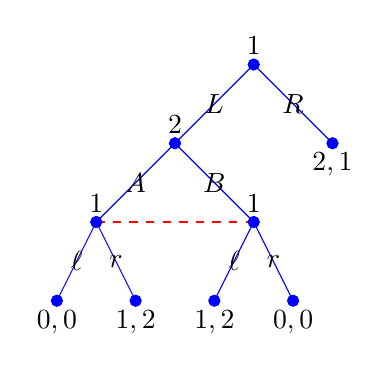
\begin{tikzpicture}
			\draw[red,dashed,thick] (-2,-2)--(0,-2);
			\filldraw[blue] (0,0) circle(2pt);
			\filldraw[blue]  (1,-1) circle(2pt);
			\filldraw[blue]  (-1,-1) circle(2pt);
			\filldraw[blue]  (-2,-2) circle(2pt);
			\filldraw[blue]  (0,-2) circle(2pt);
			\filldraw[blue]  (.5,-3) circle(2pt);
			\filldraw[blue]  (-.5,-3) circle(2pt);
			\filldraw[blue]  (-1.5,-3) circle(2pt);
			\filldraw [blue] (-2.5,-3) circle(2pt);
			
			\draw[blue] (-2.5,-3)--(-2,-2)--(-1,-1)--(0,0)--(1,-1);
			\draw[blue] (-1,-1)--(0,-2)--(.5,-3);
			\draw[blue] (0,-2)--(-.5,-3);
			\draw[blue] (-1.5,-3)--(-2,-2);
			
			
			\node[below] at (1,-1) {$2,1$};
			\node[below] at (-1.5,-3) {$1,2$};
			\node[below] at (-2.5,-3) {$0,0$};
			\node[below] at (-.5,-3) {$1,2$};
			\node[below] at (.5,-3) {$0,0$};
			\node[above] at (0,0) {$1$};
			\node[above] at (-1,-1) {$2$};
			\node[above] at (-2,-2) {$1$};
			\node[above] at (0,-2) {$1$};
			\node at (0.5,-0.5) {$R$};
			\node at (-0.5,-0.5) {$L$};
			\node at (-1.5,-1.5) {$A$};
			\node at (-0.5,-1.5) {$B$};
			\node at (-1.75,-2.5) {$r$};
			\node at (.25,-2.5) {$r$};
			\node at (-.25,-2.5) {$\ell$};
			\node at (-2.25,-2.5) {$\ell$};
		\end{tikzpicture}
	\end{figure}
	Here, $P(\emptyset) = P(L,A) = P(L,B) = 1$, and $P(L) = 2$. $\mathscr{I}_1 = \{\emptyset ,\{(L,A),(L,B)\}\}$, $\mathscr{I}_2 = \{\{L\}\}$.
\end{example}

\begin{definition}

With this model, we can describe games in which players \blue{play simultaneously} -- these are equivalent to situations in which players play sequentially but do not observe the other's actions. Information partitions are a primitive of the game, but they can be refined by using reasoning.
\end{definition}

\begin{example}
	\red{Game with imperfect recall} Think of the following single-player game, often called \red{The Forgetful Driver}:
	
	\begin{figure}[H]
		\centering
		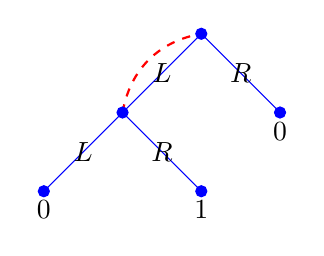
\begin{tikzpicture}
			\draw[red,dashed,thick] (-1,-1) to[out=80,in=190](0,-0);
			\filldraw[blue] (0,0) circle(2pt);
			\filldraw[blue]  (1,-1) circle(2pt);
			\filldraw[blue]  (-1,-1) circle(2pt);
			\filldraw[blue]  (-2,-2) circle(2pt);
			\filldraw[blue]  (0,-2) circle(2pt);
			\draw[blue] (1,-1)--(0,0)--(-1,-1)--(-2,-2);
			\draw[blue] (0,-2)--(-1,-1);
			\node at (-0.5,-0.5) {$L$};
			\node at (0.5,-0.5) {$R$};
			\node at (-1.5,-1.5) {$L$};
			\node at (-0.5,-1.5) {$R$};
			\node[below] at (1,-1) {$0$};
			\node[below] at (0,-2) {$1$};
			\node[below] at (-2,-2) {$0$};
		\end{tikzpicture}
	\end{figure}
\end{example}

\begin{definition}
	An extensive game has \blue{perfect recall} if for each player $i$ we have $X_i(h) = X_i(h')$ if $h$ and $h'$ are in the same information set of $i$. Note that in the above example, we have that $X_1(\emptyset) = \{\emptyset,L\} \ne \{\{\emptyset,L\},\{L\}\} = X_1(L)$.
\end{definition}

\begin{definition}
	A \blue{pure strategy} of player $i$ in an extensive game is a function mapping each information set $I_i$ to an action $A_i(I_i)$.
\end{definition}

\begin{definition}
	We say that two games are \blue{strategically equivalent} if they have the same strategic form. Formally:
\end{definition}
\begin{theorem}\label{thm:thomson_strategic}
	(from \href{https://www.rand.org/content/dam/rand/pubs/research_memoranda/2009/RM759.pdf}{Thomson, 1952}) The following transformations on the extensive form preserve the strategic form:
	\begin{enumerate}
		\item Inflation-deflation
		\item Coalescing of moves
		\item Interchange of moves
		\item Addition of superfluous moves
	\end{enumerate}
\end{theorem}
\begin{proof}
	Proof follows immediately from defining the four transformations:
	\begin{enumerate}
		\item \blue{Inflation-deflation} means that $\Gamma$ is equivalent to $\Gamma'$ if (i) $\Gamma'$ differs from $\Gamma$ only in that there is an information set in $\Gamma'$ that is a union of information sets in $\Gamma$, and (ii) any two histories $h$ and $h'$ in different members of the union have subhistories that are in the same information set of player $i$, and in that same information set player $i$'s action is not equal in $h$ and $h'$.
		\item \blue{Coalescing of moves} is natural and direct, just combining when one player moves twice in a row, as it is outcomes that matter rather than sequences of moves.
		\item \blue{Interchange of moves} basically says that the order of moves is immaterial when players do not see the other's action.
		\item \blue{Addition of superfluous moves} naturally does not change anything about the game.
	\end{enumerate}
\end{proof}

We also have the following:
\begin{corollary}
	(aslo from \href{https://www.rand.org/content/dam/rand/pubs/research_memoranda/2009/RM759.pdf}{Thomson, 1952}) If two finite extensive games are strategically equivalent, and neither contains an information set that contains both a history $h$ and a subhistory of $h$, one can be attained from the other by a sequence of the four transformations in Theorem~\ref{thm:thomson_strategic}.
\end{corollary}


\subsection{Mixed and Behavioral Strategies}

We have two ways to describe a mixed strategy in an extensive game:

\begin{definition}
	A \blue{mixed strategy} of player $i$ in an extensive game is a probability measure over the set of player $i$'s pure strategies.
\end{definition}
\begin{definition}
	A \blue{behavioral strategy} of player $i$ in an extensive game is a collection $\{\beta_i(I_i)\}_{I_i \in \mathscr{I}_i}$ of independent probability measures, where $\beta_i(I_i)$ is a probability measure over $A(I_i)$.
\end{definition}

\begin{example}
	\red{Mixed Strategies} Consider the following game:
	\begin{figure}[H]
		\centering
		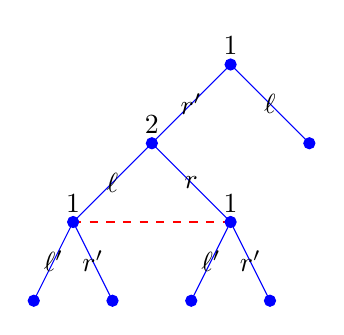
\begin{tikzpicture}
			\draw[thick, red, dashed] (-2,-2)--(0,-2);
			\filldraw[blue] (0,0) circle(2pt);
			\filldraw[blue]  (1,-1) circle(2pt);
			\filldraw[blue]  (-1,-1) circle(2pt);
			\filldraw[blue]  (-2,-2) circle(2pt);
			\filldraw[blue]  (0,-2) circle(2pt);
			\filldraw[blue]  (.5,-3) circle(2pt);
			\filldraw[blue]  (-.5,-3) circle(2pt);
			\filldraw[blue]  (-1.5,-3) circle(2pt);
			\filldraw [blue] (-2.5,-3) circle(2pt);
			\draw[blue] (-2.5,-3)--(-2,-2)--(-1,-1)--(0,0)--(1,-1);
			\draw[blue] (-1,-1)--(0,-2)--(.5,-3);
			\draw[blue] (0,-2)--(-.5,-3);
			\draw[blue] (-1.5,-3)--(-2,-2);
			\node[above] at (0,0) {$1$};
			\node[above] at (-1,-1) {$2$};
			\node[above] at (-2,-2) {$1$};
			\node[above] at (0,-2) {$1$};
			\node at (0.5,-0.5) {$\ell$};
			\node at (-0.5,-0.5) {$r'$};
			\node at (-1.5,-1.5) {$\ell$};
			\node at (-0.5,-1.5) {$r$};
			\node at (-1.75,-2.5) {$r'$};
			\node at (.25,-2.5) {$r'$};
			\node at (-.25,-2.5) {$\ell'$};
			\node at (-2.25,-2.5) {$\ell'$};
		\end{tikzpicture}
	\end{figure}
	Pure strategies assign an action to each information set, so for $1: \emptyset,\{(r,l),(r,r)\}$, and for $2: \{\{l\},\{r\}\}$. So for 1 a strategy is an ordered pair: $(r,\ell'),(r,r'),(\ell,\ell'),(\ell,r')$. A mixed strategy is a probability distribution over these strategies, and a behavioral strategy is instead a collection of $\beta_i(I_i)(a_i)$. 
\end{example}

\begin{definition}
	For any strategy profile $\sigma$, we define the \blue{outcome} $O(\sigma)$ to be to be the probability distribution over the terminal histories that results when each player $i$ follows the strategy. We will formalize this:
\end{definition}

\begin{definition}
	For any history $h = (a^1,\dots,a^k)$ define a \blue{pure strategy} $s_i$ of player $i$ to be \blue{consistent} with $h$ if for every subhistory $(a^1,\dots,a^t)$ of $h$ for which $P(a^1,\dots,a^t) = i$, we have that $s_i(a^1,\dots,a^t) = a^{t+1}$. For any history $h$, we have that $\pi_i(h)$ is the \blue{sum of the probabilities} according to $\sigma_i$ of all the pure strategies of player $i$ that are consistent with $h$. Then, for any profile of \blue{mixed strategies}, the probability that $O(\sigma)$ assigns to any terminal history $h$ is $\prod_{i \in N \cup \{c\}} \pi_i(h)$. For any profile of \blue{behavioral strategies}, the probability that $O(\sigma)$ assigns to any terminal history $h$ is $\prod_{k=0}^{K-1} \beta_{P(a^1,\dots,a^k)}(a^{k+1})$ where $a^0 = \emptyset$ by definition. Two strategies are \blue{outcome equivalent} if for any profile of pure strategies of the other players, they induce the same outcome distribution.
\end{definition}

\begin{question}
	When are mixed and behavioral strategies equivalent?
\end{question}

The most natural definition of a mixed strategy from a behavioral one is:\[\prod_{I_i\in\mathscr{I}_i} \beta_i(I_i) (s_i(I_i))\]However, this only works if the randomizations at the information sets are independent. Note that this does not work if a history and its associated sub-history are in the same information set. This property is implied by perfect recall. As an example, think about the absent-minded driver game from earlier. A mixed strategy will assign positive probability only on the two bad outcomes, because it cannot condition on the information set. However, a behavioral strategy could put positive probability on the good outcome. 


\begin{theorem}
	\red{Kuhn} For every mixed strategy of a player in a finite extensive game with perfect recall, there is an outcome-equivalent behavioral strategy.
\end{theorem}
\begin{proof}
	Recall that $\pi_i(h)$ is the sum of probabilities according to $\sigma_i$ of all the pure strategies consistent with $h$. Because we have perfect recall, if $h$ and $h'$ are in the same information set $I_i$, then $X_i(h) = X_i(h')$, so it follows that $\pi_i(h) = \pi_i(h')$. We can thus define the behavioral strategy \[\beta_i(I_i)(a) = \frac{\pi_i(h,a)}{\pi_i(h)}\]for $h \in I_i$ such that $\pi_i(h) > 0$. Note that for outcome equivalence it is irrelevant how we define $\beta_i(I_i)(a)$ when $\pi_i(h) = 0$.
\end{proof}


\begin{definition}
	A \blue{Nash equilibrium in mixed strategies} of an extensive game is a profile of mixed strategies with the property that for every player $i \in N$ we have\[O(\sigma_i\opt,\sigma_{-i}\opt) \succeq_i O(\sigma_i,\sigma_{-i}\opt)\]for any $\sigma_i$.
\end{definition}







\subsection{Sequential Equilibria}


When we studied extensive games with perfect information, it's natural to restrict to subgame perfect equilibria. The natural extension to imperfect information is to require that a Nash equilibrium is a Nash equilibrium in any information set where the player is asked to take an action. This sometimes works, and sometimes doesn't.

\begin{example}
	Consider a game where $1$ chooses $\ell,m,r$ and $2$ only sees whether they choose $\ell$ or not, and if not can choose in $\ell,r$. The game structure is Figure~\ref{fig:seq_equ_ex}.
	\begin{figure}[H]
	\centering
		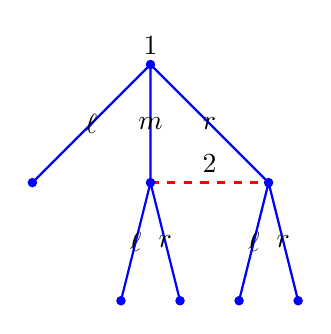
\begin{tikzpicture}[scale=1.5]
			\draw[blue,thick] (-1,-1)--(0,0)--(0,-1)--(0,0)--(1,-1);
			\draw[blue,thick] (-0.25,-2)--(0,-1)--(0.25,-2);
			\draw[blue,thick] (1.25,-2)--(1,-1)--(0.75,-2);
			\draw[red,dashed,very thick] (0,-1)--(1,-1);
			\filldraw[blue] (0,0) circle(1pt);
			\filldraw[blue] (-1,-1) circle(1pt);
			\filldraw[blue] (0,-1) circle(1pt);
			\filldraw[blue] (1,-1) circle(1pt);
			\filldraw[blue] (-0.25,-2) circle(1pt);x
			\filldraw[blue] (.25,-2) circle(1pt);
			\filldraw[blue] (.75,-2) circle(1pt);
			\filldraw[blue] (1.25,-2) circle(1pt);
			\node[above] at (0,0) {$1$};
			\node[above] at (0.5,-1) {$2$};
			\node at (-0.5,-0.5) {$\ell$};
			\node at (0.5,-0.5) {$r$};
			\node at (0,-0.5) {$m$};
			\node at (-0.125,-1.5) {$\ell$};
			\node at (0.125,-1.5) {$r$};
			\node at (1-0.125,-1.5) {$\ell$};
			\node at (1+0.125,-1.5) {$r$};
		\end{tikzpicture}
		\caption{Sequential Equilibrium Example}
		\label{fig:seq_equ_ex}
	\end{figure}
	
	
	In this case, payoffs are $(\ell,\emptyset)=(2,2)$, $(m,\ell) = (3,1)$, $(m,r) = (0,0)$, $(r,\ell) = (0,2)$, and $(r,r) = (1,1)$. In this game, $(\ell,r)$ is a Nash equilibrium, but the threat to choose $r$ is not credible -- indeed, $2$'s decision is suboptimal for any belief set, regardless of what case they're in. This is a situation where subgame perfection logic works perfectly, and gives us a clear unique SPE: $(m,\ell)$.
	
	However, if we changed the payoffs to $(m,r)$ to be $(0,2)$. Here, $2$'s optimal action depends on her beliefs at $I_2$. Choosing $r$ is optimal if at least $1/2$ probability is on $m$, otherwise it is $\ell$. We can't even construct a posterior in most cases, let alone characterize it. 
\end{example}
\begin{remark}
	Beliefs are not pinned down by strategies.
\end{remark}

\begin{remark}
	The key idea we will explore is to extend the definition of equilibrium beyond strategies, to include beliefs as an integral part of the equilibrium definition.
\end{remark}

\begin{definition}
	We define an \blue{assessment} t0 be a strategy profile and a belief system. We require that it satisfies: (i) \blue{sequential rationality}, meaning that actions are optimal given beliefs, and (ii) \blue{consistency} of beliefs with strategies and the structure of the game.
	
	Consistency requires some additional things:
	\begin{enumerate}
		\item \blue{Consistency with strategies}, meaning that beliefs are obtained by Bayes' Rule whenever possible
		\item \blue{Structural consistency}, meaning that even at information sets where Bayes' Rule has no bite, beliefs are pinned down by some strategy profile using Bayes' Rule
		\item \blue{common beliefs}, that all players have the same beliefs after unexpected events
	\end{enumerate}
\end{definition}

Formally,

\begin{definition}
	An \blue{assessment} in an extensive game is a pair $(\beta,\mu)$ where $\beta$ is a profile of behavioral strategies, and $\mu$ is a function that assigns to every information set a probability measure on the set of histories of the information set. The assessment $(\beta,\mu)$ is \blue{sequentially rational} if for every player $i \in N$ and every information set $I_i$, we have
	\[
	O((\beta,\mu);I_i) \succeq_i O((\beta_i',\beta_{-i},\mu);I_i)
	\]
	Note that this definition may generate some paradoxical results.
\end{definition}

\begin{example}
	Consider the game illustrated in Figure~\ref{fig:weird_sequential_game}. Nature chooses the path, and Players 1 and 2 do not know which path they'll be on. If player 1 would choose differently on path $A$ versus path $B$, which only requires that payoffs are slightly different, then there are no sequentially rational equilibria.
	
	
	\begin{figure}[ht]
		\centering
		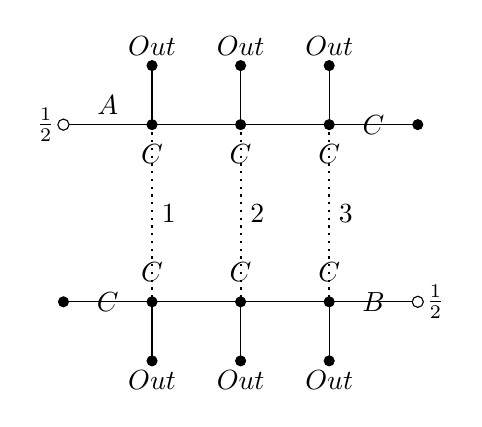
\begin{tikzpicture}[
    dot/.style={circle, fill, inner sep=0.05cm},
    empty/.style={circle, draw, inner sep=0.05cm}, scale=0.75
]

% The horizontal lines
\draw (0.1,0) -- (6,0);
\draw (0,-3) -- (5.9,-3);

% The vertical lines
\draw (1.5,0) -- (1.5,1) node[above] {$Out$};
\draw (3,0) -- (3,1) node[above] {$Out$};
\draw (4.5,0) -- (4.5,1) node[above] {$Out$};

\draw (1.5,-3) -- (1.5,-4) node[below] {$Out$};
\draw (3,-3) -- (3,-4) node[below] {$Out$};
\draw (4.5,-3) -- (4.5,-4) node[below] {$Out$};

% The nodes on the horizontal lines
\node[empty] at (0,0) {};
\node[dot] at (1.5,0) {};
\node[dot] at (3,0) {};
\node[dot] at (4.5,0) {};
\node[dot] at (6,0) {};

\node[dot] at (0,-3) {};
\node[dot] at (1.5,-3) {};
\node[dot] at (3,-3) {};
\node[dot] at (4.5,-3) {};
\node[empty] at (6,-3) {};

% The labels
\node[above] at (0.75,0) {$A$};
\node at (1.5,-0.5) {$C$};
\node[right] at (1.5,-1.5) {$1$};
\node[right] at (3,-1.5) {$2$};
\node[right] at (4.5,-1.5) {$3$};
\node at (3,-0.5) {$C$};
\node at (4.5,-0.5) {$C$};
\node at (5.25,0) {$C$};
\draw[thick, dotted] (1.5,0)--(1.5,-3);
\draw[thick, dotted] (3,0)--(3,-3);
\draw[thick, dotted] (4.5,0)--(4.5,-3);

\node at (0.75,-3) {$C$};
\node at (1.5,-2.5) {$C$};
\node at (3,-2.5) {$C$};
\node at (4.5,-2.5) {$C$};
\node at (5.25,-3) {$B$};

% The fraction labels
\node at (-0.3,0) {$\frac{1}{2}$};
\node at (6.3,-3) {$\frac{1}{2}$};

% The dots at the ends of vertical lines
\node[dot] at (1.5,1) {};
\node[dot] at (3,1) {};
\node[dot] at (4.5,1) {};

\node[dot] at (1.5,-4) {};
\node[dot] at (3,-4) {};
\node[dot] at (4.5,-4) {};

			
		\end{tikzpicture}
		\caption{A Weird Sequential Game}
		\label{fig:weird_sequential_game}
	\end{figure}
\end{example}


\begin{definition}
	An assessment $(\beta,\mu)$ is \blue{consistent} if: (i) there exists a sequence $(\beta^n,\mu^n)$ of assessments that converges to $(\beta,\mu)$ in Euclidean space; (ii) each strategy profile $\beta^n$ is completely mixed; and (iii) each belief system $\mu^n$ is derived from $\beta^n$ using Bayes' Rule.
\end{definition}

\begin{proposition}
	An assessment is a \blue{sequential equilibium} if it is sequentially rational and consistent.
\end{proposition}

\begin{example}
	Consider the same game as the first example, but with payoffs (in order) \[\{(\ell,\emptyset), (m,\ell) , (m,r) , (r,\ell),(r,r)\} \equiv \{(2,2), (3,1),(0,2),(0,2),(1,1)\}\], so player 2's optimal action depends on their beliefs. An assessment in whcih $\beta_1(\ell) = 1$ and $\beta_2(r) = 1$, and $\mu_2(\{m,r\})(m) = \alpha \ge \frac{1}{2}$ is a sequential equilibrium. 
\end{example}

\begin{example}
	Consider \red{Selten's Horse} (due to \href{https://link.springer.com/article/10.1007/BF01766400}{Selten, 1975})
	\begin{figure}[H]
	\centering
		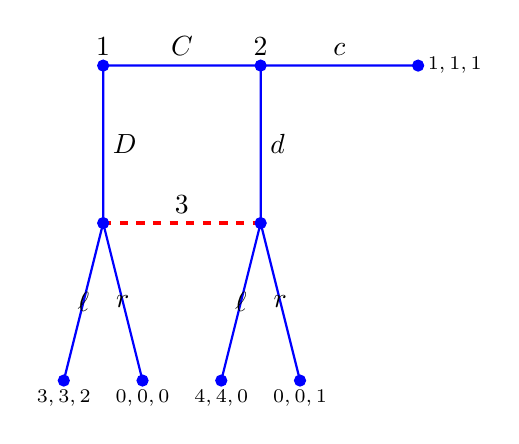
\begin{tikzpicture}[scale=2]
			\draw[blue, thick] (-.25,-2)--(0,-1)--(0,0)--(2,0);
			\draw[blue,thick] (.25,-2)--(0,-1);
			\draw[blue,thick] (1,0)--(1,-1)--(.75,-2)--(1,-1)--(1.25,-2);
			\draw[red, dashed, very thick] (0,-1)--(1,-1);
			
			
			\node[right] at (2,0) {\scriptsize$1,1,1$};
			\node[below] at (-.25,-2) {\scriptsize$3,3,2$};
			\node[below] at (.25,-2) {\scriptsize$0,0,0$};
			\node[below] at (.75,-2) {\scriptsize$4,4,0$};
			\node[below] at (1.25,-2) {\scriptsize$0,0,1$};
			\node[above] at (0.5,0) {$C$};
			\node[above] at (1.5,0) {$c$};
			\node[right] at (0,-0.5) {$D$};
			\node[right] at (1,-0.5) {$d$};
			\node at (-0.125,-1.5) {$\ell$};
			\node at (0.125,-1.5) {$r$};
			\node at (1-0.125,-1.5) {$\ell$};
			\node at (1+0.125,-1.5) {$r$};
			
			\node[above] at (0,0) {$1$};
			\node[above] at (1,0) {$2$};
			\node[above] at (0.5,-1) {$3$};
			
			\filldraw[blue] (0,0) circle(1pt);
			\filldraw[blue] (1,0) circle(1pt);
			\filldraw[blue] (2,0) circle(1pt);
			\filldraw[blue] (0,-1) circle(1pt);
			\filldraw[blue] (1,-1) circle(1pt);
			\filldraw[blue] (-.25,-2) circle(1pt);
			\filldraw[blue] (.25,-2) circle(1pt);
			\filldraw[blue] (1-.25,-2) circle(1pt);
			\filldraw[blue] (1.25,-2) circle(1pt);
		\end{tikzpicture}
	\end{figure}
	
	Here we have two types of Nash equilibria. In the first, $\beta_1(\emptyset)(D) = 1$, $\beta_2(C)(c) \in [1/3,1]$, and $\beta_3(I_3)(\ell) = 1$. In the second, $\beta_1(\emptyset)(C) = 1$, $\beta_2(C)(c) =1$, and $\beta_3(I_3)(r) \ge 3/4$. The first set are not sequential equilibria, because player 2 would deviate (making player 1's strategy not optimal). The second set are, strangely, sequentially rational, if we construct strategies limiting to the pure strategies.
\end{example}


\begin{remark}
	In a large class of interesting games, we have more structure that can be exploited to simplify the equilibrium analysis. In Bayesian extensive games with observed actions, players observe all actions in the game. All uncertainty is about the player types.
\end{remark}

\begin{definition}
	A \blue{Bayesian extensive game with observable actions} is a tuple $\langle \Gamma, \{\Theta_i\},\{p_i\},\{u_i\}\rangle$, where: (i) $\Gamma = \langle N,H,P\rangle$ is an extensive game form with perfect information and (potentially) simultaneous moves; (ii) $\Theta_i$ is the finite set of types with $\Theta = \bigtimes_i \Theta_i$; (iii) $p_i$ is a probability measure on $\Theta_i$, where assume $p_i \indep p_j$ for all $i \ne j$;\footnote{Note that, for example, the Juror game we did earlier has correlated types and so is not independent. There's actually no real reason to assume independent types.} and (iv) $u_i: \Theta \times Z \to \reals$ are von Neumann-Morgenstern utility functions, where $u_i(\theta,h)$ is the expected utility of $i$ when the types are $\theta$ and the (terminal) history is $h$.
\end{definition}

\begin{remark}
	This definition is very connected to the definition of an extensive game with imperfect information, which is a generalization of this. We could turn any Bayesian extensive game into an extensive game with imperfect information by introducing a nature that plays in the first period and decides the types. The player who assigns types will assign them with the same distribution as the probability measure over types.\footnote{This is not necessary, but often holds. Note that we defined earlier the measures as indexed by each player -- they don't even need the same support.} We define the information sets as, for any $\theta_i$, and possible $\theta_{-i}$ and any possible history $h$.
\end{remark}

In this context, an assessment is a pair $\parl\sigma,\mu\parr$, where $\sigma = \{\sigma_i(\theta_i)(h)\}_i$ and $\mu = \{\mu_i(h)\}_i$, where $\sigma_i(\theta_i)(h)$ is a probability distribution over $A_i(h)$ if $i \in P(h)$, and $\mu_i(h)$ is a probability distribution over $\Theta_i$ condition on $h$, so for players $-i$. Given $(\sigma,\mu)$, we can define \[O(\sigma_{-i},\sigma_i,\mu_{-i};h)\]

 \begin{definition}
 	For a Bayesian extensive game with observed actions, $(\sigma,\mu)$ is a \blue{Perfect Bayesian equilibrium} if: (i) it is sequentially rational, so $O(\sigma_{-i},\sigma_i(\theta_i),\mu_{-i};h) \succeq_{\theta_i}O(\sigma_{-i},s_i,\mu_{-i};h)$ for any other strategy $s_i$ of $i$ in $\Gamma$; (ii) it has \blue{correct initial beliefs}, so $\mu_i(\emptyset) = p_i$; (iii) it has \blue{action-determined beliefs} where if $i \not\in P(h)$, then $\mu_i(h,a) = \mu_i(h)$, and if $i \in P(h)$ and $a,a'\in A(h)$ with $a_i = a_i'$, then $u_i(h,a) = u_i(h,a')$; and (iv) it has \blue{Bayesian updating}, where if $i \in P(h)$ and $a_i$ is in the support of $\sigma_i(\theta_i)(h)$ for some $\theta_i$ in the support of $\mu_i(h)$, then for any $\theta_i' \in \Theta_i$: \[\mu_i(h,a)(\theta_i') = \frac{\sigma_i(\theta'_i)(h)(a_i) \cdot \mu_i(h)(\theta_i')}{\sum_{\theta_i\in \Theta_i} \sigma_i(\theta_i)(h)(a_i) \cdot \mu (h)(\theta_i)}\]
 \end{definition}

\begin{example}
	Consider a game in which nature first chooses one of two types of player 1: $(t_1,t_2)$. Each type is chosen with equal probability. Player 1 observes her type and decides whether to choose $L$ or $R$. If player 1 chooses $R$, the game ends and the payoffs are $(1,1)$, but if player 1 chooses $L$ player 2 has to choose between $T$ and $B$, without knowing the type of player 1:
	
	\begin{figure}[H]
	\centering
	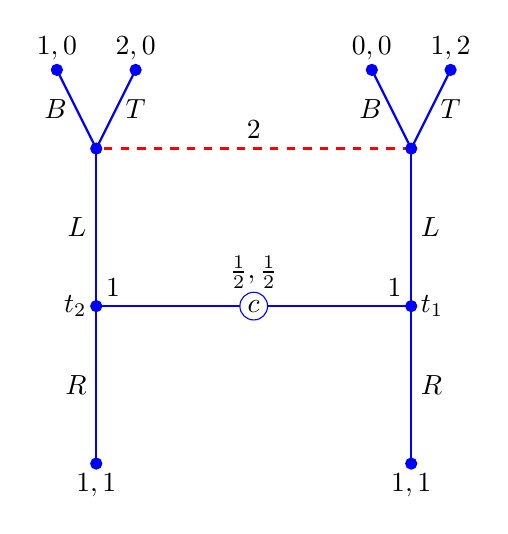
\begin{tikzpicture}
		\draw[blue,thick] (-2,2)--(-2,-2)--(-2,0)--(2,0)--(2,2)--(2,-2);
		\draw[blue,thick] (-2.5,3)--(-2,2)--(-1.5,3);
		\draw[blue,thick] (2.5,3)--(2,2)--(1.5,3);
		\draw[dashed,very thick, red] (2,2)--(-2,2);
		
		\node[right] at (2,0) {$t_1$};
		\node[right] at (2,1) {$L$};
		\node[right] at (2,-1) {$R$};
		\node[left] at (-2,1) {$L$};
		\node[left] at (-2,-1) {$R$};
		\node[left] at (-2,0) {$t_2$};
		\node[below] at (-2,-2) {$1,1$};
		\node[below] at (2,-2) {$1,1$};
		\node[right] at (-1.75,2.5) {$T$};
		\node[left] at (1.75,2.5) {$B$};
		\node[right] at (2.25,2.5) {$T$};
		\node[left] at (-2.25,2.5) {$B$};
		\node[above right] at (-2,0) {$1$};
		\node[above left] at (2,0) {$1$};
		\node[above] at (0,2) {$2$};
		\node[above] at (-2.5,3) {$1,0$};
		\node[above] at (2.5,3) {$1,2$};
		\node[above] at (-1.5,3) {$2,0$};
		\node[above] at (1.5,3) {$0,0$};
		\node[above] at (0,0.1) {$\frac{1}{2},\frac{1}{2}$};
		\filldraw [blue] (2,0) circle(2pt);
		\filldraw [blue] (-2,0) circle(2pt);
		\filldraw [blue] (2,-2) circle(2pt);
		\filldraw [blue] (-2,-2) circle(2pt);
		\filldraw [blue] (2,2) circle(2pt);
		\filldraw [blue] (-2,2) circle(2pt);
		\filldraw [blue] (-2.5,3) circle(2pt);
		\filldraw [blue] (1.5,3) circle(2pt);
		\filldraw [blue] (2.5,3) circle(2pt);
		\filldraw [blue] (-1.5,3) circle(2pt);
		\filldraw[color=blue,fill=white] (0,0) circle(5pt);
		\node (0,0) {$c$};
	\end{tikzpicture}
	\end{figure}
	
	The payoffs after histories $h = (t_1,LT),(t_1,LB)$ are respectively $(1,2)$ and $(0,0)$, and the payoffs after histories $h = (t_2,LT),(t_2,LB)$ are respectively $(2,0)$ and $(1,0)$. We can solve this game by checking 2's posterior beliefs. In the first case, we start when Player 2 always plays $T$, in which case $t_2$ always chooses $L$, and $t_2$ is indifferent -- this admits a family of equilibria, in which $\sigma_2 = 1$, $\sigma_1^2 = 1$, and $\sigma_1^1 \in [0,1]$. Next, we can consider when player 2 chooses $B$ with probability 1. Then it must be that $\mu(t_2 \mid L) = 1$, so $\sigma_1^2 \in [0,1]$ and $\sigma_1^1 = 0$. This is also an equilibrium. Note that we need to confirm that the off-path beliefs when $\sigma_1^2 = 0$ are sequentially rational, which is easily done. Finally, we check the case where $\sigma_2 \in (0,1)$. This means that player 2 is indifferent, so it must be the case that $\mu(t_2 \mid L) = 1$, so $\sigma_1^2 = 1$, and $\sigma_1^1 = 0$. All of these hold by strictly higher expected utility of the respective action. 
\end{example}


\subsection{Signaling Games}

\begin{example}
	\red{Spence's Model of Education} (from \href{https://www.jstor.org/stable/1882010}{Spence, 1973}). We saw this last semester. We have two players, a \blue{sender} and a \blue{receiver}, where the sender is informed of the value of an uncertain parameter $\theta_1$ and then chooses an action $m$ (referred to as a \blue{message}). The receiver observes the message (but not $\theta_1$) and takes an \blue{action} $a$. Each player's payoff depends on the value of $\theta_1$, the message $m$ sent by the sender, and the action $a$ taken by the receiver: $u_i(\theta_1,m,a)$. 
	
	\begin{remark}
		What makes this problem interesting is that the sender has the information, but does not take any action; the receiver controls the action but has no information.
	\end{remark}
	
	Specifically, we assume that our two players are a worker $(i=1$, sender) whose ability is $\theta_1$, where $|theta_1 \in \{\theta^L,\theta^H\}$, where $p_L$ is the probability of a low type. The employer's payoff is $u_2(\theta_1,e,w) = -(w-\theta_1)^2$, and the worker's payoff is $u_1(\theta_1,m,w) = w - \frac{e}{\theta_1}$, where $e \ge 0$ is effort. Here, $e$ is the message and $w$ is the action. 
	
	We will now show that in this game we have a pooling equilibrium with $e^H = e^L = e\opt$ and age $w\opt = \expect\{\theta_1\} = p_L \theta_1^L + (1-p_L)\theta_1^H$. This is an equilibrium in which there is no signaling, the types behave the same way. 
	
	First of all, note that the description so far is incomplete -- what beliefs follow an effort $e \ne e\opt$? For this, let's assume that $\mu(\theta_1^L) = 1$ if $e \ne e\opt$. In this case, the wage after a deviation is $w(e) =\theta_1^L$, so we have that a deviation is unprofitable if and only if\[\theta_1^L \le p_L\theta_1^L + (1-p_L) \theta_1^H - \max\curll \frac{e\opt}{\theta_1^H},\frac{e\opt}{\theta_1^L}\curlr = p_L\theta_1^L + (1-p_L)\theta_1^H - \frac{e\opt}{\theta_1^L} \iff e\opt \le \theta_1^L \cdot p^H (\theta_1^H - \theta_1^L) \]So this is a perfect Bayesian equilibrium. But is the assumption on out of equilibrium beliefs consistent? Let's consider the fully mixed strategies where $\sigma_1(\theta_1^L)(e\opt) = 1-\varepsilon$, $\sigma_1(\theta_1^H)(e\opt) = 1-\varepsilon^2$, $\sigma_1(\theta_1^L)(e) = \varepsilon$, and $\sigma_1(\theta_1^H)(e) = \varepsilon^2$, for any $e \ne e\opt$. Then we have that \[\mu(\theta_1^L ; e,\sigma) = \frac{\varepsilon p_L}{\varepsilon^2 (1-p_L) + \varepsilon p_L} \to 1 \text{ as } \varepsilon\to0\]We can thus conclude that the pooling equilibria are sequential equilibria.
	
	We now will show that this game admits a separating equilibrium. In this, $e_1^L = 0$ with associated $w(e_1^L) = \theta_1^L$ and $e_1^H > 0$ with $w(e_1^H) = \theta_1^H$. We will assume that beliefs are $\mu(\theta_1^L) = 1$ if $e < e_1^H$. For this to be an equilibrium, we need that neither type will deviate. This happens as long as \[\theta_1^L \ge \theta_1^H - \frac{e^H_1}{\theta_1^L} \qquad \text{ and } \qquad \theta_1^H - \frac{e^H}{\theta^H_1} \ge \theta_1^L\]These conditions combine to:\[\theta_1^L \cdot p^H (\theta_1^H - \theta_1^L) \le e^H \le \theta_1^H \cdot p^H (\theta_1^H - \theta_1^L)\]We can prove that this is a sequential equilibrium with the exact same strategy as above, constructing a sequence of fully mixed strategies that converge to the pure strategies. 
\end{example}


\begin{question}
	Are there ways to refine these equilibria?
\end{question}
\begin{remark}
	Consider the following game:
	\begin{figure}[H]
		\centering
		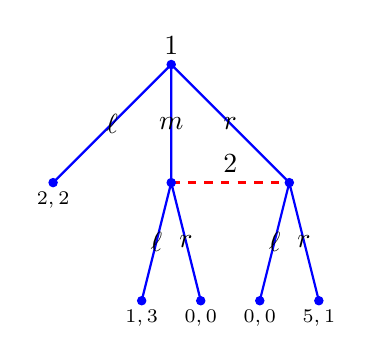
\begin{tikzpicture}[scale=1.5]
			\draw[blue,thick] (-1,-1)--(0,0)--(0,-1)--(0,0)--(1,-1);
			\draw[blue,thick] (-0.25,-2)--(0,-1)--(0.25,-2);
			\draw[blue,thick] (1.25,-2)--(1,-1)--(0.75,-2);
			\draw[red,dashed,very thick] (0,-1)--(1,-1);
			\filldraw[blue] (0,0) circle(1pt);
			\filldraw[blue] (-1,-1) circle(1pt);
			\filldraw[blue] (0,-1) circle(1pt);
			\filldraw[blue] (1,-1) circle(1pt);
			\filldraw[blue] (-0.25,-2) circle(1pt);x
			\filldraw[blue] (.25,-2) circle(1pt);
			\filldraw[blue] (.75,-2) circle(1pt);
			\filldraw[blue] (1.25,-2) circle(1pt);
			\node[above] at (0,0) {$1$};
			\node[above] at (0.5,-1) {$2$};
			\node at (-0.5,-0.5) {$\ell$};
			\node at (0.5,-0.5) {$r$};
			\node at (0,-0.5) {$m$};
			\node at (-0.125,-1.5) {$\ell$};
			\node at (0.125,-1.5) {$r$};
			\node at (1-0.125,-1.5) {$\ell$};
			\node at (1+0.125,-1.5) {$r$};
			\node[below] at (-1,-1) {\scriptsize$2,2$};
			\node[below] at (-.25,-2) {\scriptsize$1,3$};
			\node[below] at (.25,-2) {\scriptsize$0,0$};
			\node[below] at (.75,-2) {\scriptsize$0,0$};
			\node[below] at (1.25,-2) {\scriptsize$5,1$};
		\end{tikzpicture}
	\end{figure}
	This game has a sequential equilibrium with outcome $(r,r)$. Player 2 believes that $r$ is chosen with probability 1. This game also has a sequential equilibrium with outcome $(\ell,\ell)$, where player 2 believes that $m$ is chosen with high probability. The second equilibrium has a problem: $m$ is strictly dominated by $\ell$ for Player 1. Hence, if Player 2 is ever called to act, they should believe that $r$ was necessarily the choice by Player 1.
\end{remark}

\begin{example}
	\red{Beer and Quiche} Consider the following classic signaling game, in Figure~\ref{fig:beer_and_quiche}. 
	
	\begin{figure}[ht]
	\centering
	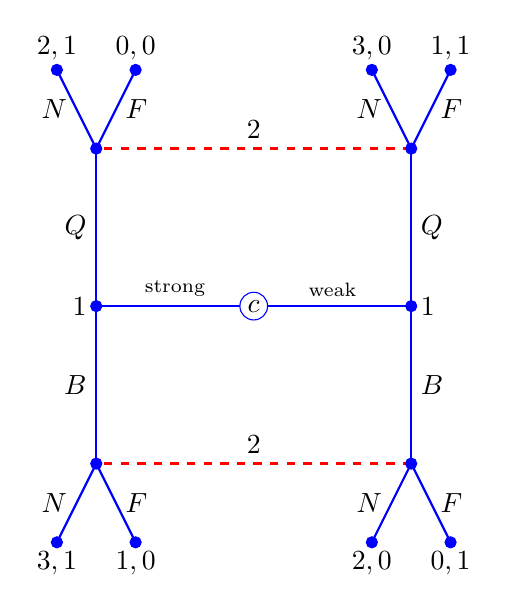
\begin{tikzpicture}
		\draw[blue,thick] (-2,2)--(-2,-2)--(-2,0)--(2,0)--(2,2)--(2,-2);
		\draw[blue,thick] (-2.5,3)--(-2,2)--(-1.5,3);
		\draw[blue,thick] (2.5,3)--(2,2)--(1.5,3);
		\draw[blue,thick] (-2.5,-3)--(-2,-2)--(-1.5,-3);
		\draw[blue,thick] (2.5,-3)--(2,-2)--(1.5,-3);
		\draw[dashed,very thick, red] (2,2)--(-2,2);
		\draw[dashed,very thick, red] (2,-2)--(-2,-2);
		
		\node[right] at (2,1) {$Q$};
		\node[right] at (2,-1) {$B$};
		\node[left] at (-2,1) {$Q$};
		\node[left] at (-2,-1) {$B$};
		\node[right] at (-1.75,2.5) {$F$};
		\node[left] at (1.75,2.5) {$N$};
		\node[right] at (2.25,2.5) {$F$};
		\node[left] at (-2.25,2.5) {$N$};
		\node[right] at (-1.75,-2.5) {$F$};
		\node[left] at (1.75,-2.5) {$N$};
		\node[right] at (2.25,-2.5) {$F$};
		\node[left] at (-2.25,-2.5) {$N$};
		\node[left] at (-2,0) {$1$};
		\node[right] at (2,0) {$1$};
		\node[above] at (0,2) {$2$};
		\node[above] at (0,-2) {$2$};
		\node[above] at (-1,0) {\scriptsize strong};
		\node[above] at (1,0) {\scriptsize weak};
		\node[above] at (-2.5,3) {$2,1$};
		\node[above] at (2.5,3) {$1,1$};
		\node[above] at (-1.5,3) {$0,0$};
		\node[above] at (1.5,3) {$3,0$};
		\node[below] at (-2.5,-3) {$3,1$};
		\node[below] at (2.5,-3) {$0,1$};
		\node[below] at (-1.5,-3) {$1,0$};
		\node[below] at (1.5,-3) {$2,0$};
		\filldraw [blue] (2,0) circle(2pt);
		\filldraw [blue] (-2,0) circle(2pt);
		\filldraw [blue] (2,-2) circle(2pt);
		\filldraw [blue] (-2,-2) circle(2pt);
		\filldraw [blue] (2,2) circle(2pt);
		\filldraw [blue] (-2,2) circle(2pt);
		\filldraw [blue] (-2.5,3) circle(2pt);
		\filldraw [blue] (1.5,3) circle(2pt);
		\filldraw [blue] (2.5,3) circle(2pt);
		\filldraw [blue] (-1.5,3) circle(2pt);
		\filldraw [blue] (-2.5,-3) circle(2pt);
		\filldraw [blue] (1.5,-3) circle(2pt);
		\filldraw [blue] (2.5,-3) circle(2pt);
		\filldraw [blue] (-1.5,-3) circle(2pt);
		\filldraw[color=blue,fill=white] (0,0) circle(5pt);
		\node (0,0) {$c$};
	\end{tikzpicture}
	\caption{Beer and Quiche}
	\label{fig:beer_and_quiche}
	\end{figure}
	
	The strong type has probability $0.9$. There are two classes of equilibria: (i) both types of player 1 choose $B$; player 2 fights if he observes $Q$ and not if he observes $B$ (so if player 2 observes $Q$, he puts probability at least 0.5 that player 1 is weak), and (ii) both types of player 1 choose $Q$; player 2 fights if he observes $B$ and not if he observes $Q$ (so if player 2 observes $B$, he puts probability at least 0.5 that player 1 is weak).
	
	We will rule out the second class of equilibria. To do so, ask who benefits from a deviation. If a weak type deviates, he obtains less in equilibrium no matter what player 2 does. On the contrary, if 1 is strong and the deviation works (so player 2 selects $N$), then she benefits. Maybe it is instead reasonable to assume that player 2 would treat any deviation as a strong type. 
\end{example}

\begin{remark}
	We can apply the above ideas to Spence's education model. Consider an $e'$ such that:\[\expect\{\theta\} - \frac{e\opt}{\theta_1^L} \ge \theta_1^H - \frac{e'}{\theta_1^L} \qquad \text{ and } \qquad \expect\{\theta\} - \frac{e\opt}{\theta_1^H} < \theta_1^H - \frac{e'}{\theta_1^H}\]where $e\opt$ is a pooling equilibrium. Since a low type is worse off if believed, but a high type is better off. Given this, a receiver would believe that a deviator is a high type, so there are no pooling equilibria.
	
	Next, consider a separating equilibrium where $e_L = 0$, $e_H > 0 \st \theta^H_1 - \frac{e^H}{\theta^H_1} \ge \theta_1^L$. Assume that the inequality is strict. If the receiver sees a deviation to $e'$ such that $e' < e^H$ but $\theta^H_1 - \frac{e'}{\theta^H_1} \ge \theta_1^L$, a high type benefits from the deviation if believed, but a low type does not benefit from deviating, so the receiver will conclude that the deviation comes from a high type. We can conclude that there is only one separating equilibrium that survives, in which $e^L = 0$ and $e^H$ is such that $\theta^H_1 - \frac{e^H}{\theta^H_1} = \theta_1^L$.
\end{remark}


\subsection{Trembling Hand Perfect Equilibria}

We next consider the robustness of an equilibrium to small perturbations in the equilibrium strategies. Recall that a strategy is \blue{completely mixed} if it assigns positive probability to all actions.

\begin{definition}
	A \blue{trembling hand perfect equilibrium} of a finite strategic game is a mixed strategy profile $\sigma$ with the property that there exists a sequence $\{\sigma^k\}_{k=0}^\infty$ of completely mixed strategy profiles that converges to $\sigma$ such that for all players $i$ the strategy $\sigma_i$ is a best response to $\sigma_{-i}^k$ for all values of $k$. Note that $\sigma$ must be a Nash equilibrium. 
\end{definition}

We can see that this is stronger than Nash equilibrium -- in the following game, $(B,B)$ is the only THPE:
\begin{center}
	\begin{tabular}{c|ccc}
		& A & B & C \\\hline
		A & $(0,0)$ & $(0,0)$ & $(0,0)$ \\
		B & $(0,0)$ & $(1,1)$ & $(2,0)$ \\
		C & $(0,0)$ & $(0,2)$ & $(2,2)$ \\
	\end{tabular}
\end{center}

\begin{remark}
	We cannot have a trembling hand perfect equilibrium that places positive probability on a weakly dominated action. For two player games, this is even tighter:
\end{remark}
\begin{proposition}
	A strategy profile in a finite two-player strategic game is a trembling hand perfect Nash equilibrium if and only if it is a mixed strategy Nash equilibrium that places no positive probability on weakly dominated actions.
\end{proposition}
\begin{remark}
	This does not hold with more than two players. Consider:
	\begin{center}
		\begin{tabular}{c|cc}
			& $L$ & $R$ \\\hline 
			$T$ & $(1,1,1)$ & $(1,0,1)$ \\
			$B$ & $(1,1,1)$ & $(0,0,1)$
		\end{tabular}
		\qquad
		\begin{tabular}{c|cc}
			& $L$ & $R$ \\\hline 
			$T$ & $(1,1,0)$ & $(0,0,0)$ \\
			$B$ & $(0,1,0)$ & $(1,0,0)$
		\end{tabular}
	\end{center}
	\[
	\ell \qquad\qquad\qquad\qquad\qquad\qquad\qquad r
	\]
	where Player 1 plays the rows, Player 2 plays the columns, and Player 3 chooses the matrix. The Nash equilibrium $(B,L,\ell)$ is not weakly dominated but not trembling hand perfect.
\end{remark}



\begin{proposition}
	Every finite strategic game has a trembling hand perfect equilibrium
\end{proposition}
\begin{proof} 
	(Intuitive, skipping some details). Define a perturbation of the game by letting the set of actions of each player $i$ be the set of mixed strategies of player $i$ that assign probability of at least $\varepsilon_j^i$ to each action $j$ of player $i$, for some collection $\{\varepsilon_j^i\}$ with $\varepsilon_j^i > 0 \forall i,j$. That is, we constrain each player to use each action available with some minimum probability.
	
	We can see easily that there is a Nash equilibrium in each of these games, since the best response correspondences are never empty.\footnote{Proof follows from the standard argument using the standard Fixed Point Theorems, noting that the strategy sets are compact and the best response correspondence is upper hemi-continuous.} Take $\varepsilon_j^i \to 0$ for each $i,j$ in sequence. By compactness of the set of strategy profiles, we have that there is a converging subsequence of strategies, converging to some $\sigma\opt$ in the original game. This is a Trembling Hand Perfect Equilibrium.
\end{proof}

\begin{remark}
	We can extend THPE to extensive games, but we have some issues. Consider the following game in extensive and normal form:
	\begin{figure}[H]
	\centering
		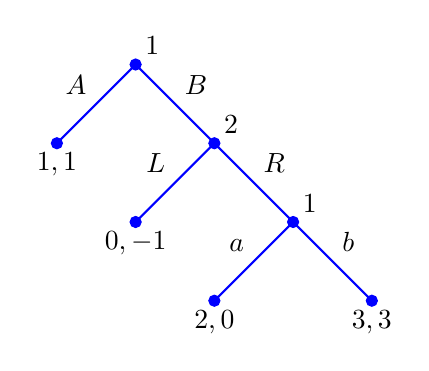
\begin{tikzpicture}
			\draw[blue,thick] (-1,-1)--(0,0)--(1,-1)--(0,-2)--(1,-1)--(2,-2)--(1,-3)--(2,-2)--(3,-3);
			\filldraw[blue] (0,0) circle(2pt);
			\filldraw[blue] (-1,-1) circle(2pt);
			\filldraw[blue] (1,-1) circle(2pt);
			\filldraw[blue] (2,-2) circle(2pt);
			\filldraw[blue] (3,-3) circle(2pt);
			\filldraw[blue] (1,-3) circle(2pt);
			\filldraw[blue] (0,-2) circle(2pt);
			\node[above right] at (0,0) {$1$};
			\node[above right] at (1,-1) {$2$};
			\node[above right] at (2,-2) {$1$};
			\node[above left] at (-0.5,-0.5) {$A$};
			\node[above right] at (0.5,-0.5) {$B$};
			\node[above left] at (0.5,-1.5) {$L$};
			\node[above right] at (1.5,-1.5) {$R$};
			\node[above left] at (1.5,-2.5) {$a$};
			\node[above right] at (2.5,-2.5) {$b$};
			\node[below] at (-1,-1) {$1,1$};
			\node[below] at (0,-2) {$0,-1$};
			\node[below] at (1,-3) {$2,0$};
			\node[below] at (3,-3) {$3,3$};
		\end{tikzpicture}
	\end{figure}
	\begin{center}
		\begin{tabular}{c|cc}
			& $L$ & $R$ \\\hline 
			$A,a$ & $1,1$ & $1,1$ \\
			$A,b$ & $1,1$ & $1,1$ \\
			$B,a$ & $0,2$ & $2,0$ \\
			$B,b$ & $0,2$ & $3,3$ 
		\end{tabular}
	\end{center}
	$(B,b),R$ is the unique subgame perfect equilibrium, so it seems plausible as the choice for the trembling hand perfect equilibrium. However, $(A,a),L$ is also a trembling hand perfect equilibrium of the normal form of the game. The problem arises because 1 does not consider the possibility that \emph{she} will make a mistake when evaluating the strategies, she only considers that 2 will make a mistake. If she considers the fact that she will make mistakes, $a$ is never optimal. 
	
	This motivates studying the trembling hand perfect equilibria in the \blue{agent strategic form} rather than the strategic (normal) form of the game. 
\end{remark}

\begin{definition}
	The \blue{agent strategic form} of an extensive form game is a game where there is one player for each information set in the extensive form game. Each player in the extensive game is split into a number of agents, one for each of his information sets, all agents of a given player having the same payoffs.
	
	A mixed strategy $\sigma(I_i)$ of the agent strategic form corresponds to a behavioral strategy $\beta(I_i)$ of the corresponding game. This motivates:
\end{definition}

\begin{definition}
	A trembling hand perfect equilibrium of a finite extensive game is a behavioral strategy profile that corresponds to a trembling hand perfect equilibrium of the agent strategic form of the game.
\end{definition}


\section{Knowledge}

\subsection{Modeling Knowledge}

\begin{model}
	In a \red{model of knowledge}, we must have states $\Omega$, an information function corresponding to what an agent knows, and a notion of knowledge:
	\begin{enumerate}
		\item States describe contingencies that are relevant for a particular decision. Here, a state is a complete description of the world, including an agent's information, beliefs, and prior actions. States are exactly as before
		\item An information function for $\Omega$ is a function $h$ that associates with each state $\omega \in \Omega$ a nonempty subset $h(\omega)$ of $\Omega$. We interpret $h(\omega)$ as the set of states that an agent considers possible at $\omega$. This is actually more primitive than a signaling function, as this gives only information over the state, not types. \\\\An information function is \blue{partitional} if there is some partition of $\Omega$ such that for any $\omega \in \Omega$, $h(\omega)$ is the element of the partition that contains $\omega$. An information function is partitional if and only if it satisfies the following two properties: (i) $\omega \in h(\omega)$ for every $\omega \in \Omega$, and (ii) if $\omega' \in h(\omega)$, then $h(\omega')=h(\omega)$.
		\item We will say that the agent \blue{knows} $E \subseteq \Omega$ if $E$ obtains at all of the states that the agent thinks are possible. We refer to a set of states $E \subseteq \Omega$ as an event where (i) if $h(\omega) \subseteq E$, then in state $\omega$, the agent views $\neg E$ as impossible. We define the agent's \blue{knowledge function} $K$ by $K(E) = \{\omega\in \Omega : h(\omega) \subseteq E\}$, as the states where the agent knows $E$.
	\end{enumerate}
\end{model}

\begin{remark}
	Notice that for every state $\omega \in \Omega$, we have that $h(\omega) \subseteq \Omega$. Therefore it follows that:
\end{remark}
\begin{axiom}
	\red{Axiom of Awareness} $K(\Omega) = \Omega$
\end{axiom}
\begin{axiom}
	\red{Axiom of Intersection} $K(E) \cap K(F) = K(E\cap F)$
\end{axiom}
\begin{axiom}
	\red{Axiom of Knowledge} If the information function is partitional,\footnote{A typical assumption.} $K(E) \subseteq E$
\end{axiom}
\begin{axiom}
	\red{Axiom of Transparency} If the information function is partitional, $K(E) \subseteq K(K(E))$
\end{axiom}
\begin{axiom}
	\red{Axiom of Wisdom} $\Omega \setminus K(E) \subseteq K(\Omega \setminus K(E))$
\end{axiom}



The intuitions are:
\begin{enumerate}
	\item Regardless of the actual state, the agent knows he is in some state
	\item If you know two things, you know you must be in a state where both of them are simultaneously true
	\item The agent cannot know something that is false
	\item If the agent knows something, he knows that he knows something (note that this inducts)
	\item If the agent does not know something, he knows that he does not know it
\end{enumerate}

\begin{definition}
	Suppose that there are $I$ agents with partitional information functions $h_1,\dots,h_I$ and associated knowledge functions $K_1,\dots,K_I$. We say that an event $E\subseteq \Omega$ is \blue{mutual knowledge} in state $\omega$ if it is known to all agents, meaning that\[\omega \in K_1(E) \cap K_2(E) \cap \cdots \cap K_I(E) \equiv K^1(E)\]An event is \blue{common knowledge} in state $\omega$ if it is known to everyone, everyone knows this, everyone knows that everyone knows this, and so on.
\end{definition}

\begin{remark}
	Note that $K^1(K^1(E)) \in K^1(E)$, and this inducts. We could formalize the above definition as:
\end{remark}
\begin{definition}
	An event $E \subseteq \Omega$ is \blue{common knowledge} in state $\omega$ if \[\omega \in K^1(E) \cap K^1(K^1(E)) \cap K^1(K^1(K^1(E))) \cap \cdots\]
\end{definition}


\begin{example}
	Suppose $\Omega = \{\omega_1,\omega_2,\omega_3,\omega_4\}$ and there are two individuals with information partitions \[H_1 = \{\{\omega_1\},\{\omega_2,\omega_3\},\{\omega_4\}\} \qquad ;\qquad H_2 = \{\{\omega_1,\omega_2\},\{\omega_3\},\{\omega_4\}\}\]We can see that $E = \{\omega_1,\omega_2\}$ is never common knowledge because it does not contain any self-evident event. However, the event $\{\omega_1,\omega_2\}$ can be mutual knowledge in state $\omega_1$, since $K_1(\{\omega_1,\omega_2\}) = \{\omega_1\} \in \{\omega_1,\omega_2\} = K_2(\{\omega_1,\omega_2\})$.
	
	Note also that $F = \{\omega_1,\omega_2,\omega_3\}$ is common knowledge, since it is self-evident. This provides a cleaner definition:
\end{example}

\begin{definition}
	We say that an event $F$ is \blue{self-evident} if for all $\omega \in F$ and $i = 1,\dots,I$, we have $h_i(\omega) \subseteq F$.
\end{definition}
\begin{definition}
	An event $E \subseteq \Omega$ is common knowledge in state $\omega \in \Omega$ if there is a self-evident event $F$ for which $\omega \in F \subseteq E$.
\end{definition}

\begin{lemma}
	The following are equivalent:
	\begin{enumerate}
		\item $K_i(E) = E$ for all $i$
		\item $E$ is self-evident
		\item $E$ is a union of members of the partition induced by $h_i$ for all $i$
	\end{enumerate}
\end{lemma}
\begin{proof}
	To see that (1) and (2) are equivalent, note that $F$ is self-evident if and only if $F \subseteq K_i(F)$ for all $i$. By the Axiom of Knowledge, $K_i(F) \subseteq F$ always, so $F$ is self-evident if and only if $K_i(F) = F$ for all $i$.
	
	To see that (2) implies (3), note that if $E$ is self-evident, then $\omega \in E$ implies that $h_i(\omega) \subseteq E$, so $E = \bigcup_{\omega \in E} h_i(\omega)$ for all $i$.
	
	(3) implying (1) is immediate.
\end{proof}

\begin{proposition}
	The two definitions of common knowledge are equivalent.
\end{proposition}
\begin{proof}
	Assume $E$ is common knowledge at $\omega$ according to the first definition, so $E \supseteq K^1(E) \supseteq K^1(K^1(E)) \supseteq \cdots$ and $\omega$ is a member of each of those sets, which are thus nonempty. Since $\Omega$ is finite, there is some set $F = K^1(K^1(K^1(\cdots K^1(E)\cdots)))$ for which $K_i(F) = F$ for all $i$. So this set $F$ with $\omega \in F \subseteq E$ is self-evident and $E$ is common knowledge by the second definition.
	
	Assume $E$ is common knowledge at $\omega$ by the second definition, so there exists $F$ self-evident for which $\omega \in F \subseteq E$. Then $K_i(F) = F$ for all $i$, meaning that $K^1(F) = F$, and $K^1(K^1(F)) = F$, and so on. Thus, since $\omega \in F$, \[\omega \in F \subseteq K^1(E) \cap K^1(K^1(E)) \cap K^1(K^1(K^1(E))) \cap \cdots\]so $E$ is common knowledge by the first definition.
\end{proof}

\begin{example}
	\red{Aumann's Agreement Theorem} (from \href{https://www.jstor.org/stable/2958591?seq=1}{Aumann, 1976}) Could two individuals who share the same prior agree to disagree? That is, if $i$ and $j$ share a common prior over states, could a state arise in which it was commonly that: $i$ assigned probability $\eta_i$ to some event, $j$ assigned probability $\eta_j$ to that same event, and $\eta_i \ne \eta_j$? 
	
	Formally, let $p$ be a measure on $\Omega$, and for any state $\omega$ and event $E$, let $p(E \mid h_i(\omega))$ be the probability $i$ assigns to $E$ (using Bayes' Rule). The event that `$i$ assigns probability $\eta_i$ to $E$' is\[\{\omega\in\Omega : p(E \mid h_i(\omega) = \eta_i\}\]
		
	\begin{proposition}
		Suppose two agents have the same prior belief over a finite set of states $\Omega$. If each agent's information is partitional and it is common knowledge in some state $\omega \in \Omega$ that agent 1 assigns probability $\eta_1$ to some event $E$ and agent 2 assigns probability $\eta_2$ to $E$, then $\eta_1=\eta_2$.
	\end{proposition}
	\begin{proof}
		If the assumptions are satisfied, then there is some self-evident event $F$ with $\omega \in F$ such that \[F \subseteq \{\omega_0 \in \Omega : p(E \mid h_1(\omega_0) = \eta_1)\} \cap \{\omega_0\in \Omega : p(E \mid h_2(\omega_0) = \eta_2)\}\}\] Moreover, $F$ is a union of members of $i$'s information partition. Since $\Omega$ is finite, say that $F = \bigcup_k A_k^1 =\bigcup_k A_k^2$. Now for any non-empty disjoint sets $C,D$ with $p(E \mid C) = \eta_i$ and $p(E \mid D) = \eta_i$, we must have that $p(E \mid C \cup D) = \eta_i$. For each $k$, we have that $p(E \mid A_k^i) = \eta_1$, so \[p(E \mid F) = p(E \mid \bigcup_k A_k^1) = \eta_1\]and similarly, \[\eta_1 = p(E \mid F) = p(E \mid \bigcup_k A_k^2) = p(E \mid A_k^2) = \eta_2\]Thus, the two cannot be different.
	\end{proof}
\end{example}

\begin{example}
	\red{The No-Trade Theorem} (from \href{https://web.stanford.edu/~milgrom/publishedarticles/Information\%20Trade\%20and\%20Common\%20Knowledge.pdf}{Milgrom \& Stokey, 1982}) Suppose there are two agents. Let $\Omega$ be a set of states and $X$ a set of consequences, which are trading outcomes.
	
	\begin{definition}
		A \blue{contingent contract} is a function that maps $\Omega$ to $X$.
	\end{definition}
	Let $A$ be the space of contracts $a: \Omega \to X$. Each agent has a utility function $u_i: X \times \Omega \to \reals$. Let $U_i(a) = u_i(a(\omega),\omega)$ denote $i$'s utility from a contract. Note that $U_i(a)$ is a random variable dependent on $\omega$. Let $\expect[U_i(a) \mid H_i]$ denote $i$'s expected utility conditional on his information $H_i$, and say that a contract is \blue{ex ante efficient} if it is (in expectation) Pareto efficient.
\end{example}
\begin{theorem}
	If a contingent contract $b$ is ex ante efficient, then it cannot be common knowledge between the agents that every agent prefers contract $a$ to contract $b$.
\end{theorem}
\begin{proof}
	The claim is that there cannot be a state $\omega$ which occurs with positive probability in which the set\[E = \{\omega : \expect[U_i(a)\mid h_i(\omega)] \ge \expect[U_i(b) \mid h_i(\omega)] \forall i\}\](with strict inequality holding for at least one $i$) is common knowledge. Suppose FSOC that there is such a state $\omega$ and hence a self-evident set $F$ such that $\omega \in F \subseteq E$. By the definition of self-evident sets, for all $\omega'\in F$ and all $i$, $h_i(\omega') \subseteq F$, so for all $\omega'\in F$ and all $i$, \[\expect[U_i(a) - U_i(b) \mid h_i(\omega')] > 0\]and using the fact that $i$'s information is partitional, we know that \[F = h_i(\omega_1) \cup h_i(\omega_2) \cup \cdots \cup h_i(\omega_n)\]for some set of states $\omega_1,\dots,\omega_n \in F$ and all $i$. It follows that for all $i$, \[\expect[U_i(a) - U_i(b) \mid F] > 0\]However, we assumed that $b$ was ex-ante efficient, and this is a Pareto improvement to $a$. Thus, we have a contradiction. 
\end{proof}

\begin{model}
	\red{The Electronic Mail Game} (from \href{https://arielrubinstein.tau.ac.il/papers/32.pdf}{Rubinstein, 1989}) This game highlights the main issues in understanding knowledge in game theory. Two players play game $G_b$ with probability $p < \frac{1}{2}$ and $G_a$ with probability $1-p$. In both games, players have actions $A,B$. The games are:
	\[G_a = \begin{array}{c|cc} & A & B \\\hline A & M,M & 1,-L \\ B & -L,1 & 0,0 \end{array}\qquad \qquad G_b =\begin{array}{c|cc} & A & B \\\hline A & 0,0 & 1,-L \\ B & -L,1 & M,M \end{array} \]In both games, it is mutually beneficial to choose the same action, but the action that is best depends on the game. In $G_a$, $(A,A)$ is best, and in $G_b$, $(B,B)$ is best. We assume that $L > M> 1$. Even if a player knows that the game is $G_b$, it is risky to choose $B$ unless she is confident her partner will play $B$ also. Player 1 knows the true game, player 2 receives an informative signal $\{a,b\}$. 
	
	If $2$'s signal is entirely uninformative, there is a unique equilibrium in which both players play $A$, where the payoff is $(1-p)M$ to each player. If the players can communicate, 1 sends a perfectly informative message, and they coordinate on $A$ in $G_a$ and $B$ in $G_b$. These are the benchmarks.
	
	Consider a variant. Players can communicate, but imperfectly. They communicate via computers, with the following protocol: If the game is $G_b$, then player 1's computer automatically sends a message to player 1's computer. If the game is $G_a$, no message is sent. If a computer receives a message ever, it sends a message back. This is for the original message, the confirmation, the confirmation of the confirmation, and so on. There is a small probability $\varepsilon > 0$ that a sent message doesn't arrive at its destination. If the message does not arrive, communication stops. At the end of communication, each player sees the number of messages \emph{her} computer has sent. We can specify states and information functions. States are:
	\[
	\Omega = \curll (Q_1,Q_2) : Q_1 = Q_2 \text{ or } Q_1 = Q_2 + 1\curlr
	\]
	In the state $(q,q)$, player 1's computer sends $q$ messages all of which arrive, and the $q$th message sent by player 2 goes astray. In the state $(q+1,q)$, player 1's computer sends $q+1$ messages, all but the last arrive at player 2's computer. Player 1's information function is defined by \[P_1(q,q) = \begin{cases} (q,q),(q,q-1) & q > 0 \\ (0,0) & q = 0\end{cases}\]Player 2's information function is \[P_2(q,q) = \{(q,q),(q+1,q)\} \forall q\]The game that is played is $G_a$ if $(0,0)$, otherwise $G_b$. 
	
	Player 1 knows the game in all states, player 2 knows the game in all states except for $(0,0)$ and $(1,0)$. In each of the states $(1,0)$, $(1,1)$ player 1 knows that the game is $G_b$ but does not know that player 2 knows that. 
	
	In each of the states $(1,1)$ and $(2,1)$, player 2 knows that the game is $G_b$ but does now know whether player 1 knows that player 2 knows that the game is $G_b$, and so on.
	
	As $q$ increases, we seem to get closer to common knowledge.
	
	We can study this as a Bayesian game. The states are defined as above, and the signal function is \[\tau_i(Q_1,Q_2) = Q_i\]Each player's belief on $\Omega$ is the same, derived from the technology and the assumption that the prior probability is $p$:\begin{align*} p_i(0,0) &= 1-p \\ p_i(q+1,q) &= p\varepsilon(1-\varepsilon)^{2q} \\ p_i(q+1,q+1) &= p\varepsilon(1-\varepsilon)^{2q+1}\end{align*}The game $G(Q_1,Q_2)$ determines the payoffs. 
\end{model}
\begin{proposition}
	The electronic mail game has a unique Nash equilibrium, in which each player always chooses $A$.
\end{proposition}
\begin{proof}
	Induction, starting at $(0,0)$. In $(0,0)$, $A$ is strictly dominant for player 1, so player 1 always chooses $A$ when they receive the signal $0$. If player 2 gets no message, either player 1 did not send a message (with probability $1-p$), or they sent a message that did not arrive (with probability $p\varepsilon$). The expected payoffs are:\[ U_2(A) = \frac{(1-p)M}{1-p+\varepsilon p} \qquad ;\qquad U_2(B) = \frac{-L(1-p) + p\varepsilon M}{1-p+\varepsilon p}\]So it is strictly optimal for player 2 to choose $A$ when their signal is $0$. 
	
	Assume that the conclusion holds for all $(Q_1,Q_2)$ where $Q_1 + Q_2 \le 2q$. Consider player 1's decision when she has sent $q$ messages. She is uncertain whether $Q_2 = q$ or $Q_2 = q-1$. The probability she assigns to $Q_2 = q-1$ is \[z = \frac{\varepsilon}{\varepsilon + (1-\varepsilon)\varepsilon} > \frac{1}{2}\]Thus, she believes that it is more likely her last message did not arrive than that player 2 received the last message. If she chooses $B$, her expected payoff is at most \[-Lz + (1-z)M < 0\]since under the inductive assumption she knows that if $Q_2 = q-1$, then player 2 chooses $A$. If she chooses $A$, she can guarantee a payoff of at least 0, so she always chooses $A$. Clearly, if player 2 knows that player 1 is choosing $A$, he will also always choose $A$. Thus, the inductive conclusion is proved for $Q_1 + Q_2 \le 2q+1$, and proof follows. Thus, each player chooses $A$ in response to any signal.
\end{proof}


\section{Mechanism Design}


\textbf{\textit{n.b.}} In real time, we rushed through this section taking a lot of prior knowledge as given. This has some justification, since we learned some last semester, but if taken exactly as presented would be a bad section of notes. Instead, I've attempted to synthesize what I know of mechanism design with what Marco taught, to get a comprehensive (likely \emph{over}-comprehensive) section. I've also attempted to unify the notation because it got confusing. 


\begin{remark}
	So far, we've used the typical solution methods in Game Theory to find play patterns: take the rules of the game as given, and find what players will optimally do under those rules. We will now take a step more abstract, and think of ourselves not as a player but as a designer. Taking players (and optimal play!) as given, the question we will be solving is how to \emph{design} the rules of a game to get certain outcomes.
\end{remark}

\subsection{Selling Mechanisms}

\begin{model}
	We will generally think of problems where a seller is designing a pricing mechanism for a set of buyers, each with different preferences. The buyer has a type that they observe but the seller does not. We will broadly take the type to be the \blue{value} the buyer has for the object, where a higher type indicates a higher willingness to pay. The seller has constant marginal costs, the buyer has an outside option of value 0, and the buyer's preferences are additively separable (\blue{quasilinear}) over their value for the object and a transfer $T$. For simplicity, we will assume that values are linear in types, so the value to an agent $\theta_i$ of an allocation $q_i$ and a transfer $T_i$ is $\theta_i \cdot q_i + T_i$. This generalizes, though not without some difficulty. We will assume the typical regularity assumptions on values, where $v(0) = 0$, $v'(q) > 0$, and $v''(q) < 0$.
\end{model}

\begin{definition}
	A \blue{mechanism} is a \blue{message space} $\mathcal{M}$ and a \blue{mapping} $h(\cdot)$ from $\mathcal{M}$ to the space of outcomes, which we write as $h(m) = (q(m),T(m))$ for all $m \in \mathcal{M}$. 
\end{definition}

\begin{definition}
	A \blue{direct revelation mechanism} is a mapping $g(\cdot)$ from the space of types to the space of outcomes, where $g(\theta_i) = (q(\theta_i),T(\theta_i))$ for all $\theta_i$. A direct revelation mechanism can also be called an \blue{allocation rule} since it maps types to outcomes. The principal (the seller) commits to offer $q(\theta_i)$ at a price $T(\theta_i)$ if the agent reports that they are type $\theta_i$.
\end{definition}

\begin{definition}
	An agent $\theta_i$ finds it \blue{incentive compatible} to report her type truthfully if and only if \[\theta_i \cdot v(q(\theta_i)) - T(\theta_i) \ge \theta_i\cdot  v(q(\theta_i')) - T(\theta_i')\]for all $\theta_i' \in \Theta$. Note that as the type space increases, this condition becomes more strict. With a continuum of types, this is a continuum of conditions that must all hold.
\end{definition}

\begin{definition}
	A direct revelation mechanism $g(\cdot)$ is \blue{truthful} if it is incentive compatible for \emph{every type} of agent to announce her true type. A direct revelation mechanism $g(\cdot)$ is \blue{individually rational} if $\theta_i \cdot v(q(\theta_i)) - T(\theta_i) \ge 0$\footnote{Note that this would hold for any value to the outside auction if we set the RHS to the value of the outside option. This is why it is without loss to restrict the outside option to be zero.} for all $\theta_i$.
\end{definition}


\begin{example}
	\red{Binary Types} Let's assume that $\Theta = \{\theta_L,\theta_H\}$ with $\theta_H > \theta_L\}$ and $\prob(\theta_L) = \beta$, and constant cost to the seller $c$. We will solve this problem considering only truthful and individually rational direct revelation mechanisms. The seller's problem is: \[\max_{T,q} \beta \parl T(\theta_L) - c\cdot q(\theta_L)\parr + (1-\beta)\parl T(\theta_H) - c\cdot q(\theta_H)\parr\]subject to \begin{align*} \theta_L \cdot v(q(\theta_L)) - T(\theta_L) &\ge \theta_L \cdot v(q(\theta_H)) - T(\theta_H) &&(\text{IC}_L) \\\theta_H \cdot v(q(\theta_H)) - T(\theta_H) &\ge \theta_H \cdot v(q(\theta_L)) - T(\theta_L) &&(\text{IC}_H) \\\theta_H \cdot v(q(\theta_H)) - T(\theta_H) &\ge 0 &&(\text{IR}_H) \\ \theta_L \cdot v(q(\theta_L)) - T(\theta_L) &\ge 0 &&(\text{IR}_L)\end{align*}Note first that IR$_L$ and IC$_H$ together imply IR$_H$, since we assume that $\theta_H > \theta_L$:\[\theta_H \cdot v(q(\theta_H)) - T(\theta_H) \ge \theta_H \cdot v(q(\theta_L)) - T(\theta_L) > \theta_L \cdot v(q(\theta_L)) - T(\theta_L) \ge 0\]We next consider a relaxed version of this program where we ignore IC$_L$:\[\max_{T,q} \beta \parl T(\theta_L) - c\cdot q(\theta_L)\parr + (1-\beta)\parl T(\theta_H) - c\cdot q(\theta_H)\parr\]subject to \begin{align*} \theta_H \cdot v(q(\theta_H)) - T(\theta_H) &\ge \theta_H \cdot v(q(\theta_L)) - T(\theta_L) &&(\text{IC}_H)  \\ \theta_L \cdot v(q(\theta_L)) - T(\theta_L) &\ge 0 &&(\text{IR}_L)\end{align*}The value of this program is not less than the one above, so if the solution here still satisfies IC$_L$, the solution will solve the original problem as well. 
	
	Note that if either of the two constraints are strict inequalities, we could increase either $T(\theta_L)$ or $T(\theta_H)$ without violating anything. This would increase the payoff while maintaining feasibility, which is a contradiction. Thus, both constraints must hold with equality. From IC$_H$, we can write \begin{align*}\theta_H \dot v(q(\theta_H)) - T(\theta_H) &= \theta_H \cdot v(q(\theta_L)) - T(\theta_L) \\ &= \theta_L \cdot v(q(\theta_L)) - T(\theta_L) + (\theta_H-\theta_L)\cdot v(q(\theta_L)) \\ &= (\theta_H-\theta_L)\cdot v(q(\theta_L))\end{align*}Substituting this and the individual rationality constraint, the seller's program becomes the unconstrained\[\max_{T,q} \beta \parl \theta_L \cdot v(q(\theta_L)) - c\cdot q(\theta_L)\parr + (1-\beta) \parl \theta_H \cdot v(q(\theta_H)) - c\cdot q(\theta_H) - (\theta_H - \theta_L) \cdot v(q(\theta_L))\parr\]Note that the objective function is not necessarily concave: with the objective function defined as $W$, we have that \begin{align*} W_{q(\theta_H),q(\theta_H)} &= (1-\beta)(\theta_H \cdot v''(q(\theta_H))) < 0 \\ W_{q(\theta_H),q(\theta_L)} &= W_{q(\theta_L),q(\theta_H)} = 0 \end{align*}So this problem is concave if and only if\[W_{q(\theta_L),q(\theta_L)} = \beta(\theta_L \cdot v''(q(\theta_L)) - (1-\beta)(\theta_H - \theta_L) \cdot v''(q(\theta_L)) < 0\]Which holds only if $\beta$ is sufficiently large or if $\theta_H - \theta_L$ is sufficiently small. For now, assume that concavity is satisfied. Our first order conditions are\[\theta_H \cdot v'(q(\theta_H)) = c \qquad \text{ and } \qquad \theta_L \cdot v'(q(\theta_L)) = \frac{c}{1-\parl \frac{1-\beta}{\beta}\frac{\theta_H-\theta_L}{\theta_L}\parr}\]Note that $q(\theta_H) > q(\theta_L)$ necessarily. For this to be a solution, we need that IC$_L$ is satisfied. From IC$_H$, we have \begin{align*} \theta_H \cdot v(q(\theta_H)) - T(\theta_H) &= \theta_H \cdot v(q(\theta_L)) - T(\theta_L) \\ &\Longrightarrow \theta_H \barl v(q(\theta_H)) - v(q(\theta_L))\barr = T(\theta_H) - T(\theta_L) \\ &\Longrightarrow \theta_L \barl v(q(\theta_H)) - v(q(\theta_L))\barr \le T(\theta_H) - T(\theta_L)\end{align*}Which implies directly IC$_L$:\[\theta_L \cdot v(q(\theta_L)) - T(\theta_L) \ge \theta_L \cdot v(q(\theta_H)) - T(\theta_H)\]We can conclude that the solution to the relaxed problem is a solution to the original problem. 
	
	\begin{question}
		Why did we want until the end to establish IC$_L$? Because we needed that $q(\theta_H) \ge q(\theta_L)$ for the argument. 
	\end{question}
	Thus, the solution is:\[\theta_H \cdot v'(q(\theta_H)) = c \qquad \text{ and } \qquad \theta_L \cdot v'(q(\theta_L)) = \frac{c}{1-\parl \frac{1-\beta}{\beta}\frac{\theta_H-\theta_L}{\theta_L}\parr}\]Note that high types buy more than low types, high types buy the efficient quantity while low types buy less than efficient, and the low type receives a surplus of zero while the high type receives a positive surplus.
\end{example}


\begin{remark}
	Any mechanism $m(\cdot)$ induces an allocation rule, as long as it is optimal. Let:\[m\opt(\theta) \in \argmax_{m\in\mathcal{M}} \theta \cdot v(q(m)) - T(m)\]Then the mechanism $m$ induces the allocation rule $a(\theta) = q(m\opt(\theta)),T(m\opt(\theta))$The seller's problem is to find the mechanisms that induce the profit maximizing allocation rule. The space of mechanisms is impossibly complex, however. We can reduce it with the following:
\end{remark}

\begin{theorem}
	\red{Revelation Principle} Any possible allocation rule $a(\theta)$ obtained with a mechanism $\{\mathcal{M},h(\cdot)\}$ can also be implemented with a truthful direct revelation mechanism.
\end{theorem}
\begin{proof}
	We will show that if an outcome function is implemented by a mechanism, it can also be implemented by a direct mechanism. Take a mechanism $\{\mathcal{M},h(\cdot)\}$ that induces an outcome function\[a(\theta) = q(m\opt(\theta)),T(m\opt(\theta))\]Construct the functions $\hat{q} = q \circ m\opt$ and $\hat{T} = T \circ m\opt$, so that \[\hat{q}(\theta),\hat{T}(\theta) = q(m\opt(\theta)),T(m\opt(\theta))\]This is a direct mechanism that implements the outcome $a(\theta)$. It remains to show that this is a truthful mechanism. Since\[m\opt(\theta_i) \in \argmax_{m \in \mathcal{M}} \theta_i \cdot v(q(m)) - T(m)\]we must have that\[\theta_i \cdot v(q(m\opt(\theta_i))) - T(m\opt(\theta_i)) \ge \theta_i \cdot v(q(m\opt(\theta_j))) - T(m\opt(\theta_j)) \Longrightarrow \theta_i \cdot v(\hat{q}(\theta_i)) - \hat{T}(\theta_i) \ge \theta_i \cdot v(\hat{q}(\theta_j)) - \hat{T}(\theta_j)\]for any $\theta_i,\theta_j$. So this mechanism is truthful!
\end{proof}


\begin{remark}
	These concepts can also be applied to more complicated problems, specifically (i) problems without complete information and (ii) optimal taxation problems. In general, the structure of those problems is similar to the example above, with some complications. We will move on in these notes for time constraints.
\end{remark}

\subsection{Optimal Contracts}

\begin{remark}
	We will restrict attention here to finite types. The extension to infinite types is not trivial, and necessitates showing that the indirect utility function is integrable over types, meaning that mechanisms must be compact. However, the extension is largely technical and does not add intuition over the case of finite types. 
\end{remark}

\begin{model}
	\red{Optimal Contracts with Finite Types} We will extend the baseline model in two directions: more than two types, and a more general utility function. Formally, say that a monopolist sells a good $q$ at a price $T$, where the good is produced at a cost $C(q)$, where $C$ is convex in $q$. We assume that there are $n$ types among the buyers: $\theta_1,\theta_2,\dots,\theta_n$, where we assume WLOG that $\theta_i < \theta_j$ for $i < j$. We also assume that the probability of type $i$ is $p_i$, where $\sum_{i=1}^n p_i = 1$. We additionally adopt a more general utility function, of the form $u(q,\theta)-T$. We will assume the \blue{single-crossing property}: for $q,q',\theta,\theta'$ such that $q < q'$ and $\theta < \theta'$, \begin{align*} u(q',\theta) - u(q,\theta) > 0 &\Longrightarrow u(q',\theta') - u(q,\theta') > 0 \\u(q',\theta) - u(q,\theta) \ge 0 &\Longrightarrow u(q',\theta') - u(q,\theta') \ge 0\end{align*}Recall from math that whenever $u(q,\theta)$ is differentiable in $q$ and $\theta$, this is precisely equivalent to assuming that $u_{q\theta}(q,\theta) \ge 0$. 
\end{model}

\begin{remark}
	This has a nice interpretation in the state space $q,T$. The slope of an indifference curve is $\frac{\partial T}{\partial q} (q,\theta) = u_q(q,\theta)$, so if we have single-crossing then the slope is monotonically non-decreasing in $\theta$. 
\end{remark}

\begin{remark}
	We can still apply the revelation principle in this more general environment.
\end{remark}

The seller's problem is \[\max_{T_i,q_i} \sum_{i=1}^n p_i\parl T_i - C(q_i)\parr\]subject to\begin{align*} u(q_i,\theta_i) - T_i &\ge u(q_j,\theta_i) - T_j \forall i,j &&(\text{IC}_{i,j}) \\ u(q_i,\theta_i) - T_i &\ge 0 \forall i &&(\text{IR}_i)\end{align*}What makes this problem complex is that we have a lot of constraints: $n(n-1)+n$. We will first show a result that simplifies this to $2(n-1)+n$ constraints only. 

\begin{proposition}
	Assuming the single crossing condition, incentive compatibility is satisfied if and only if the local incentive constraints are satisfied, meaning that \begin{align*} u(q_i,\theta_i) - T_i &\ge u(q_{i-1},\theta_i) - T_{i-1} \forall i > 1 \\ u(q_i,\theta_i) - T_i &\ge u(q_{i+1},\theta_i) - T_{i+1} \forall i < n\end{align*}
\end{proposition}
\begin{proof}
	These are clearly necessary. We will prove that they are sufficient. First, note that the local IC constraints imply a monotonic allocation rule, meaning that $q_i > q_j$ as long as $i > j$: \[u(q_i,\theta_i) - u(q_{i-1},\theta_i) \ge T_i - T_{i-1} \ge u(q_i,\theta_{i-1}) - u(q_{i-1},\theta_{i-1}) \Longleftrightarrow u(q_i,\theta_i) - u(q_i,\theta_{i-1}) \ge u(q_{i-1},\theta_i) - u(q_{i-1},\theta_{i-1})\]which holds only if $q_i \ge q_{i-1}$. Consider the downward constraints, for $i$ and $i-1$: \begin{align*} u(q_i,\theta_i) - u(q_{i-1},\theta_i) &\ge T_i-T_{i-1} \\ u(q_{i-1},\theta_{i-1}) - u(q_{i-2},\theta_{i-1}) &\ge T_{i-1}-T_{i-2}\\ \Longrightarrow u(q_i,\theta_i) - u(q_{i-1},\theta_i) + u(q_{i-1},\theta_{i-1}) - u(q_{i-2},\theta_{i-1}) &\ge T_i - T_{i-2} \end{align*}Note that single-crossing implies that \[u(q_i,\theta_i)- u(q_{i-1},\theta_i) + u(q_{i-1},\theta_{i-1}) - u(q_{i-2},\theta_{i-1}) \le \underbrace{u(q_i,\theta_i)- u(q_{i-1},\theta_i) + u(q_{i-1},\theta_{i}) - u(q_{i-2},\theta_{i})}_{u(q_i,\theta_i) - u(q_{i-2},\theta_i)}\]So we have that the downward local incentive compatibility constraints imply incentive compatibility for $i$ and $i-2$:\[u(q_i,\theta_i) - u(q_{i-2},\theta_i) \ge T_i - T_{i-2}\]so proof follows through induction. We can conclude that the downward local incentive compatibility constraints imply all downward incentive compatibility constraints, and a similar argument would show the same for the upward constraints.
	
	Consider the following relaxed problem:\[\max_{T_i,q_i} \sum_{i=1}^n p_i(T_i - C(q_i))\]subject to \begin{align*} u(q_i,\theta_i) - T_i &\ge u(q_{i-1},\theta_i) - T_{i-1} \forall i > 1 \\ u(q_1,\theta_1)-T_1 &\ge 0 \\ q_i &> q_j \forall i > j\end{align*}Note that feasibility in this problem is a superset of feasibility in the original problem, since the other constraints imply monotonicity. It remains to show that the solution to this problem is feasible in the unrelaxed problem. First, note that the downward IC constraints must be binding, since if one held without equality we could raise $T_j$ for all $j$ sufficiently large without violating any constraints, and we would increase the value. With this, we can show that the solution to the relaxed problem satisfies all of the constraints of the original problem, so is feasible. This follows from the binding constraints implying that \[u(q_{i+1},\theta_{i+1}) - u(q_i,\theta_{i+1}) = T_{i+1}-T_i\]Single-crossing and monotonicity imply that\[u(q_{i+1},\theta_i) - u(q_i,\theta_i) \le T_{i+1}-T_i\]and so for all $i$,\[u(q_i,\theta_i)-T_i \ge u(q_{i+1},\theta_i) - T_i\]
\end{proof}

With this proposition, we can characterize the optimal contract by solving\[\max_{T_i,q_i} \sum_{i=1}^n p_i(T_i - C(q_i))\]subject to \begin{align*} u(q_i,\theta_i) - T_i &= u(q_{i-1},\theta_i) - T_{i-1} \forall i > 1 \\ u(q_1,\theta_1)-T_1 &= 0 \\ q_i &> q_j \forall i > j\end{align*}We can write\[T_i - C(q_i) = u(q_i,\theta_i) - C(Q_i) - (u(q_i,\theta_i) - T_i) = S(q_i,\theta_i) - U(\theta_i)\]defining $S(q_i,\theta_i)$ as the surplus generated and $U(\theta_i)$ as the indirect utility of agent $i$. Using the binding constraints, we have\[U(\theta_i) = u(q_i,\theta_i) - T_i = u(q_{i-1},\theta_i) - T_{i-1} = U(\theta_{i-1}) + \barl u(q_{i-1},\theta_i) - u(q_{i-1},\theta_{i-1})\barr\]Thus, our problem bceomes\[\max_{U_i,q_i} \sum_{i=1}^n p_i\parl S(q_i,\theta_i) - U(\theta_i)\parr\]subject to\begin{align*} U(\theta_i) &= U(\theta_{i-1}) + \barl u(q_{i-1},\theta_i) - u(q_{i-1},\theta_{i-1})\barr \forall i > 1 \\ U(\theta_1) &= 0 \\ q_i &> q_j \forall i > j\end{align*}Define the \blue{informational advantage} as the rent a type $i$ gains over a type $i-1$ as\[\Phi(q_{i-1},\theta_i,\theta_{i-1}) = u(q_{i-1},\theta_i) - u(q_{i-1},\theta_{i-1})\]Solving for $U$ recursively, we have \[U(\theta_1) = 0 \quad \text{ and } \quad U(\theta_2) = U(\theta_1) + \Phi(q_1,\theta_2,\theta_1) \quad \Longrightarrow \quad U(\theta_2) = \Phi(q_1,\theta_2,\theta_1)\]so in general\[U(\theta_i) = \sum_{j=2}^i \Phi(q_{j-1},\theta_i,\theta_{i-1})\]One way to solve this is to insert the formula for $U$ into the objective function and obtain\[\max_{U_i,q_i} \sum_{i=1}^n p_i \parl S(q_i,\theta_i) - \sum_{j=2}^i \Phi(q_{j-1},\theta_i,\theta_{i-1})\parr \st q_i > q_j \forall i > j\](where we use the convention that $\Phi(q_0,\theta_i,\theta_0) = 0$). Additionally using the convention that $\Phi(q_n,\theta_{n+1},\theta_n) = 0$, this becomes \[\max_{U_i,q_i} \sum_{i=1}^n p_i \parl S(q_i,\theta_i) - \parl 1 - \sum_{k=1}^i p_k\parr \Phi(q_{i},\theta_{i+1},\theta_{i})\parr \st q_i > q_j \forall i > j\]Generally, people assume that the monotonicity constraint can be ignored, which we will verify below. People also assume that the objective function is quasi-concave, which we will just assume. If both of those hold, the optimum is characterized by\[S'(q_i,\theta_i) - \frac{1 - \sum_{k=1}^i p_k}{p_i} \Phi'(q_i,\theta_{i+1},\theta_i) = 0 \Longrightarrow u_q(q_i,\theta_i) = C'(q) + \frac{1- \sum_{k=1}^i p_k}{p_i}\barl u_q(q_i,\theta_{i+1})-u_q(q_i,\theta_i)\barr\]for all $i < n$, and\[S'(q_i,\theta_i) = 0 \Longrightarrow u_q(q_i,\theta_i) = C'(q) \forall i = n\]

Assuming some functional forms, where $u(q,\theta) = q\cdot \theta$ and $C(q) = \frac{q^2}{2}$, we have\[\theta_i-q_i - \frac{1 - \sum_{k=1}^i p_k}{p_i} \barl \theta_{i+1}-\theta_i\barr = 0 \Longrightarrow q_i = \theta_i - \frac{1 - \sum_{k=1}^i p_k}{p_i} \barl \theta_{i+1}-\theta_i\barr  \forall i < n \]and $q_n = \theta_n$. 

\begin{remark}
	Note that we have no distortion at the top, but this phenomenon concerns only a type with probability $p_n$. All types below the highest are distorted downwards, meaning they are sold less than efficient quantities. It remains to check monotonicity. If we have $\theta_{i+1}-\theta_i = \Delta \theta$, then we have \[q_i = \theta_i - \frac{1 - \sum_{k=1}^i p_i}{p_i} \Delta \theta\]so a sufficient condition for monotonicity is that $\frac{1 - \sum_{k=1}^i p_i}{p_i}$ is non-increasing in $i$.
\end{remark}


\subsection{Optimal Auctions}

\begin{remark}
	The goal of the designer here is to design an auction that is \blue{optimal}, meaning that it maximizes revenues. The seminal work here is \href{https://www.jstor.org/stable/3689266?seq=1}{Myerson (1981)}.
\end{remark}

\begin{model} \red{Canonical Auctions} 
	We assume independent, private values, where we have $I$ bidders with preferences $v_i \cdot \phi_i - t_i$, where $v_i$ is the marginal valuation, $\phi_i$ is the probability that $i$ receives the good, and $t_i$ is the expected payment. Bidders have a reservation utility $U_i$, which for simplicity we assume is zero for all $i$. Assume that $v_i$ is drawn i.i.d. from $P_i(\cdot)$ which has support $[\underline{v},\bar{v}]$, density $p_i(v_i)$ and $p_{-i}(v_{-i}) = \prod_{j\ne i} p_i(v_i)$. The seller has a valuation $v_0$ for the good.
	
	We will look for direct mechanisms $\phi_i(v)$, $t_i(v)$ that maps type reports to an allocation, and finally the allocation must be feasible so that $\sum_i \phi_i(v) \le 1$.
\end{model}

\begin{definition}
	Denote \[\phi_i(v_i) = \expect_{v_{-i}} \phi_i(v) \qquad \text{ and } \qquad t_i(v_i) = \expect_{v_{-i}} t_i(v)\]The \blue{indirect utility function} of a type $v_i$ who reports $\hat{v}_i$ is:\[U_i(\hat{v}_i;v_i) = \phi_i(\hat{v}_i)\cdot v_i - t_i(\hat{v}_i)\]Let $U_i(v_i) \coloneqq U_i(v_i;v_i)$. The \blue{truth-telling condition} (\blue{IC})\[U_i(v_i) \ge U_i(\hat{v}_i;v_i) \forall \hat{v}_i,v_i\]
\end{definition}

Our first result is:
\begin{proposition}
	An auction mechanism where $\phi_i(v_i)$ is continuous with an absolutely continuous first derivative is incentive compatible if and only if:\[\frac{\partial U_i(v_i)}{\partial v_i} = \phi_i(v_i) \qquad \text{ and } \qquad \phi_i(v_i) \text{ is nondecreasing in } v_i\]
\end{proposition}
\begin{proof}
	The principal's problem is to solve \[\max_{t; \phi \in \Delta} \expect_v \barl \parl 1 - \sum_i \phi_i(v_i)\parr v_0 + \sum_i t_i(v_i)\barr\]subject to incentive compatibility and individual rationality. Since $t_i(v_i) = \phi_i(v_i)v_i - U_i(v_i)$, this becomes\[\max_{t;\phi\in\Delta} \expect_v \barl \parl 1 - \sum_i \phi_i(v_i)\parr v_0 \sum_i \phi_i(v_i)\cdot v_i - \sum_i U_i(v_i)\barr\]subject to IC and IR. We can rewrite the expected indirect utility function as \begin{align*} \expect_v \barl U_i(v_i)\barr &= \int_0^1 U_i(x)p_i(x)dx \\ &= - \barl U_i(x)\barl 1 - P_i(x)\barr \right|_0^1 + \int_0^1 U_i'(x) \frac{1-P_i(x)}{p_i(x)}p_i(x)\;\partial x\\ &= U_i(0) + \int_0^1 \phi_i(x) \frac{1-P_i(x)}{p_i(x)}p_i(x)\;\partial x\end{align*}Substituting the incentive compatibility constraints, the problem becomes\[\max_{t;\phi\in\Delta} \expect_v \barl \parl 1 - \sum_i \phi_i(v_i)\parr v_0 + \sum_i \phi_i(v_i)v_i - \sum_i \parl \phi_i(v_i) \frac{1-P_i(v_i)}{p_i(v_i)} + U_i(0)\parr\barr\]subject to $\phi_i(v_i)$ monotonically increasing and individual rationality. Alternatively,\[\max_{U_i(0);\phi\in\Delta} \expect_v \barl v_0 + \sum_i \phi_i(v) \parl v_i - \frac{1-P_i(v_i)}{p_i(v_i)} - v_0\parr\barr\]subject to $\phi_i(v_i)$ monotonic. 
\end{proof}



\begin{remark}
	The implication here is that all auctions that induce the same allocation of the good and that provide the same rents to types 0 generate the same expected revenues to the seller. 
\end{remark}

\begin{remark}
	\blue{The First Price Auction} (or \blue{Dutch Auction}) is a mechanism that allocates the good to the bidder with the highest value and provides zero utility to the buyer with the lowest type.
	
	\blue{The Second Price Auction} (or \blue{English Auction}) is a mechanism that allocates the good to the bidder with the highest value and provides zero utility to the buyer with the lowest type (at least when we look at equilibria in weakly undominated strategies).
	
	The implication is that they must generate the same revenues. These are examples of the following famous theorem:
\end{remark}

\begin{theorem}
	\red{The Revenue Equivalence Theorem} The seller's expected utility from an implementable auction is completely determined by the allocation function $\phi$ and the reservation utilities $U_i(0)$. 
\end{theorem}
\begin{proof}
	Follows immediately from the revelation principle. The proof of this is really lovely, see the Myerson paper for details.
\end{proof}


\begin{question}
	What is the revenue-maximizing auction?
\end{question}
\begin{remark}
	Recall that given reservation utilities, the problem is formulated as\[\max_{\phi\in\Delta} \expect_v \barl v_0 + \sum_i \phi_i(v) \parl v_i - \frac{1-P_i(v_i)}{p_i(v_i)} - v_0 \parr - \sum_i U_i(0)\barr\]subject to $\phi_i(v_i)$ being monotonic. We need only to choose $\phi \in \Delta$. Define the \blue{virtual utility} as $J_i(v_i) = v_i - \frac{1-P_i(v_i)}{p_i(v_i)}$. We proceed casewise. If $\max_i J_i(v_i) < v_0$, then set $\sum_i \phi_i(v) =0$, meaning do not sell the good. If $\max_i J_i(v_i) \ge v_0$, then allocate the good to the bidder(s) with the highest virtual utility. It remains to show that monotonicity is satisfied. A sufficient condition for this is that $\frac{1-P_i(v_i)}{p_i(v_i)}$ is non-increasing in $v_i$. 
\end{remark}

\begin{remark}
	In a symmetric environment where $P_i(v) = P_J(v)$, the standard auctions are all optimal. However, revenue equivalence fails when distributions are asymmetric. 
\end{remark}

\begin{remark}
	All of the analysis above assumes risk neutral bidders. If bidders are risk-averse instead, revenue equivalence does not hold. The first price auction will generally outperform the second price auction. Since a bidder's bid is closer to the price they pay, there is less uncertainty, which leads to more aggressive bids. An advantage of the second price auction is that it has an equilibrium with a stronger equilibrium concept, but a problem is that there are other Nash equilibria not in weakly undominated strategies. There is a `collusive' equilibrium in which the good is sold to someone at a price of zero.
	
	See \href{https://pubs.aeaweb.org/doi/pdfplus/10.1257/aer.20160425}{Li (2017)} for an exploration and extension of the differences between these auctions.
\end{remark}

























\end{document}